\documentclass[11pt,twoside,a4paper,titlepage]{article}
%%%%%%% Standart settings %%%%%%%
\usepackage{amsmath}
\usepackage{amssymb}
\usepackage[nottoc, numbib, notlot, notlof]{tocbibind}
\usepackage{fancyhdr}
\usepackage[utf8]{inputenc} 
\usepackage[margin=2.5cm]{geometry}
\usepackage{mathtools}
\usepackage[danish]{babel}
\usepackage[svgnames]{xcolor}
\usepackage{newclude}
\usepackage{siunitx}
\usepackage{booktabs}
\usepackage{subfig}
\usepackage{wrapfig} 
\usepackage[subfigure]{tocloft}
\usepackage{todonotes}
\usepackage{lastpage} 
\usepackage{lipsum,lastpage}  
\usepackage{hanging}
\usepackage{tabularx}
\setlength{\headheight}{15pt}
\usepackage{filecontents}
\usepackage{longtable}
\usepackage{footnote}
\setcounter{tocdepth}{3} % Antal lag i indholdsfortegenlse.
\setcounter{secnumdepth}{5} % Antal lag i sektioner.
\usepackage[toc,page]{appendix} % appendices
\usepackage{gensymb}
\usepackage{chngcntr}
\counterwithin{figure}{section}
\counterwithin{table}{section}
\counterwithin{equation}{section}





\usepackage{paralist}
  \let\itemize\compactitem
  \let\enditemize\endcompactitem
  \let\enumerate\compactenum
  \let\endenumerate\endcompactenum
  \let\description\compactdesc
  \let\enddescription\endcompactdesc
  \pltopsep=1pt
  \plitemsep=1pt
  \plparsep=1pt

%%%%%%% FIGURES %%%%%%%
\usetikzlibrary{positioning} % in the preamble
\usetikzlibrary{decorations.pathreplacing}
\usetikzlibrary{arrows,shapes}
\usepackage{tikz-timing}
\usepackage{graphics}
\usepackage{siunitx}
\usepackage{tikz}
\usetikzlibrary{shapes,arrows,chains, scopes}
\usepackage{pgfplots}
\usepackage{tabu}

\pgfplotsset{compat=1.8} % Burde være understøttet på alle maskiner.
\usepackage[americanvoltages, americancurrents, americanresistors, americaninductors, smartlabels]{circuitikz}
\usepackage{graphicx} % bruges til MATLAB figurer samt formatet .eps
\usepackage{epstopdf} % bruges til automatisk konvertering af .eps-filer til pdf; Ellers kan man ikke kompilere med pdfLaTeX.
\usepackage{mathtools}
\usetikzlibrary{arrows,automata} % for drawing state machines

%%%%%%% captions settings %%%%%%%
\usepackage[round]{natbib}
\bibliographystyle{plainnat}

%%%%%%% captions settings %%%%%%%
\usepackage{caption}
\captionsetup{font=footnotesize}

%%%%%%% implementering af code %%%%%%%
\usepackage{listings}
\lstset{frame=tb,
tabsize=4,
language=C,
captionpos=b,
tabsize=3,
frame=false,
numbers=left,
numberstyle=\tiny,
numbersep=5pt,
breaklines=true,
showstringspaces=false,
basicstyle=\ttfamily,
% identifierstyle=\color{magenta},
keywordstyle=\color[rgb]{0,0,1},
commentstyle=\color{ForestGreen}\ttfamily,
morecomment=[l][\color{brown}]{\#},
stringstyle=\color{red}
}
%Figurtekst under kode udsnit
\renewcommand\lstlistingname{Kodeudsnit}

%%%%%%% Diverse %%%%%%%
\usepackage{icomma}
\usepackage{pdfpages}
\usepackage[pdftex,
 hyperfigures=true,
 pdfauthor={Forfattere},
 pdftitle={},
 pdfsubject={},
 pdfkeywords={},
 hidelinks,
 plainpages=false,
 pdfpagelabels,
 unicode]{hyperref}
 
\usepackage{textcomp,gensymb} % Tilføjer et grader-tegn i mat-mode

\newenvironment{changemargin}[2]{%
\begin{list}{}{%
\setlength{\topsep}{0pt}%
\setlength{\leftmargin}{#1}%
\setlength{\rightmargin}{#2}%
\setlength{\listparindent}{\parindent}%
\setlength{\itemindent}{\parindent}%
\setlength{\parsep}{\parskip}%
}%
\item[]}{\end{list}}
%Should be used in every task diagram.
%usage is eg. 
% \node[task_description] (id)  at (0,0) {content};
% \node[task_title] at (id.north) {title};


\tikzset{buffer/.style={ %add lines
    fill=blue!10, text=black, text width = 4.5em, minimum height =3em, text centered,
    append after command={
      [shorten >=0.2bp, shorten <=0.2bp]
      (\tikzlastnode.north west)edge[very thick](\tikzlastnode.north east)
    },
    append after command={
      [shorten >=0.2bp, shorten <=0.2bp]
      (\tikzlastnode.south west)edge[very thick](\tikzlastnode.south east)
    }
  }
}
\tikzset{buffer_sem/.style={ %add lines
    fill=blue!10, text=black, text width = 4.5em, minimum height =3em, text centered,
    append after command={
      [shorten >=0.2bp, shorten <=0.2bp]
      (\tikzlastnode.north west)edge[very thick](\tikzlastnode.north east)
    },
    append after command={
      [shorten >=0.2bp, shorten <=0.2bp]
      (\tikzlastnode.south west)edge[very thick](\tikzlastnode.south east)
    },
    append after command={
      node[semaphore] at (\tikzlastnode.north east) {}
    }
  }
}
\tikzset{memory_sem/.style= {
    rectangle, draw, very thick, fill=blue!10, text width = 4.5em, minimum height =3em, text centered,
    append after command={
      node[semaphore] at (\tikzlastnode.north east) {}
    }
  }
}
\tikzstyle{memory} = [rectangle, draw, very thick, fill=blue!10, text width = 4.5em, minimum height =3em, text centered] 
\tikzstyle{interrupt} = [diamond, draw, fill=red!10, 
    text width=4.5em, text badly centered, node distance=3cm, inner sep=0pt]
\tikzstyle{task} = [circle, draw, color=black!50, text = black, fill=green!20, very thick, text width = 4.5em, minimum height = 4.5em, text centered]
\tikzstyle{task_description} = [draw, color=black!50, text=black, fill=green!10, very thick,
    rectangle, rounded corners, inner sep=10pt, inner ysep=15pt, text width = 8em, align=left]
\tikzstyle{task_title} =[fill=black!50, text=white, ellipse]

\tikzset{semaphore/.style={
   circle, draw, minimum height = 0.7cm, fill=white,
    append after command={
      (\tikzlastnode.260) --
      ++(0,0.1) edge[very thick]
      ++(0,0.5)
    },
    append after command={
      (\tikzlastnode.260) -- 
      ++(0,0.3) edge[very thick]
      ++(0.157,0.157) 
    },
    append after command={
      (\tikzlastnode.260) -- 
      ++(0,0.583) edge[very thick]
      ++(0.15,-0.15) 
    }
  }
} 

%Should be used in every controller diagram - anbae12.

\tikzstyle{block} = [draw, fill=blue!20, rectangle, minimum height=2.5em, minimum width=4em]
\tikzstyle{blockgreen} = [draw, fill=green!40, rectangle, minimum height=2.5em, minimum width=4em]
\tikzstyle{blockorange} = [draw, fill=orange!60, rectangle, minimum height=2.5em, minimum width=4em]
\tikzstyle{blocknon} = [draw, rectangle, minimum height=2.5em, minimum width=4em]
\tikzstyle{freq} = [draw, fill=green!20, ellipse, minimum height=2.5em, minimum width=3.5em]
\tikzstyle{sum} = [draw, fill=blue!20, circle, node distance=1cm]
\tikzstyle{input} = [coordinate]
\tikzstyle{output} = [coordinate]
\tikzstyle{pinstyle} = [pin edge={to-,thin,black}]
%lstlistings distance to text
\lstset{aboveskip=0pt,belowskip=-10pt} %is this too agressive?
\begin{document}

\title{Styring og regulering af et Pan \& Tilt system \\Robotteknologi 4. semesterprojekt}
\author{Gruppe 2 \\ Åse, Mikael, Mikkel, Nikolaj, Michael \& Anders}
\date{Maj 2014}
\begin{figure}
\centering

\includegraphics[width=1\textwidth]{graphics/forside.png}
\end{figure}
\maketitle



%\cleardoublepage
\clearpage
\cleardoublepage
\clearpage

% Disable indentation
\setlength{\parindent}{0pt}
\setlength{\parskip}{0.7\baselineskip}%
\pagenumbering{Roman}

\setcounter{page}{1}
\section*{Abstract}

\todo[inline,author=ALLE]{Mangler at blive skrevet}
%%%%%%%%%%%% FRONTS %%%%%%%%%%%%
%Fed \textbf{}
%Kusiv \textit{}
%Funktioner \texttt{}
%URL \url{}

%%%%%%%%%%%% PUNKTER/NUMMER %%%%%%%%%%%%
%\begin{enumerate}
%\item punkt 1
%\item punkt 2
%\end{enumerate}
%\begin{itemize}
%\item punkt
%\item punkt
%\end{itemize}


%%%%%%%%%%%% LIGNINGER %%%%%%%%%%%%
%\begin{equation}

%\label{eq:} 
%\end{equation}

%%%%%%%%%%%% FIGURER %%%%%%%%%%%%
%\begin{figure}[th!]
%\centering
%\includegraphics[width=0.4\textwidth]{./graphics/}
%\caption[tekst i indholdsfortegnelsen]{figurtekst}
%\label{fig:}
%\end{figure}	

%%%%%%%%%%%% TIKZPICTURE %%%%%%%%%%%%
%\begin{figure}[!th]
%\centering
%\begin{tikzpicture}[scale=2]
%\include*{./graphics/}
%\end{tikzpicture}
%\caption[tekst i indholdsfortegnelsen]{figurtekst}
%\label{fig:}
%\end{figure}
			
%%%%%%%%%%%% TABELLER %%%%%%%%%%%%
%\begin{figure}[th!]
%\centering
%\begin{tabular}{c|c}
%&\\\hline
%&\\
%\end{tabular}
%\captionsetup{type=table}
%\caption[tekst i indholdsfortegnelsen]{tabeltekst}
%\label{tb:}
%\end{figure}
		
%%%%%%%%%%%% STATE MACHINES DIAGRAMS %%%%%%%%%%%%
%\begin{figure}[!th]
%\centering
%\begin{tikzpicture}[scale=1,->,>=stealth',shorten >=1pt,auto,node distance=6.5cm,semithick]
%\include*{./graphics/}
%\end{tikzpicture}
%\caption[tekst i indholdsfortegnelsen]{figurtekst}
%\label{tb:}
%\end{figure}

%%%%%%%%%%%% CODE %%%%%%%%%%%%
%\begin{lstlisting}[firstnumber=???,captionpos=b, caption={filename.c/h}, label={codeex:}]

%\end{lstlisting} % Kan bruges til copy paste ind i rapport for forskellige outputs.....





\vspace{3cm}
{
\newcommand{\namesigdate}[2][5cm]{%
  \begin{tabular}{@{}p{#1}@{}}
    #2 \\[2\normalbaselineskip] \hrule \\[0pt]
%    {\small \textit{Signature}}% \\[2\normalbaselineskip] \hrule %\\[0pt]
    %{\small \textit{Date}}
  \end{tabular}
}
\begin{changemargin}{-1cm}{-1cm}
\centering
\noindent \namesigdate{Åse Videbæk Jensen} \hspace{1cm} \namesigdate{Nikolaj Iversen} \hspace{1cm} \namesigdate{Mikkel Jaedicke} \\~\\~\\
\centering
\noindent \namesigdate{Anders Launer Bæk} \hspace{1cm}  \namesigdate{Mikael Westermann} \hspace{1cm}   \namesigdate{Michael Kjær Schmidt}
\end{changemargin}
}
\bigskip
\section*{Ansvarsområder}
De primære ansvarsområder er listet i nedenstående tabel
\bigskip
\begin{table}[!th]
\centering
\setlength{\extrarowheight}{5pt}
 \begin{tabular}{r|l}
Navn&Opgaver/Ansvarsområder \\[6pt] \hline
Åse&\\
&\\[6pt] \hline
Mikkel&\\ 
&\\[6pt] \hline
Mikael&\\
&\\[6pt] \hline
Nikolaj&\\
&\\[6pt] \hline
Anders&\\
&\\[6pt] \hline
Michael & All ze errorz\\
&\\ 
\end{tabular}     
\caption*{Viser fordelingen af ansvarsområder.}            
\end{table}\\~\\ 
Det skal understreges, at tabellen er vejledende og at hele gruppen har været med over alle områder.
\todo[inline,author=Mikael]{trololol skriv ansvarsområder}
\todo[inline, author=Michael]{Yes, nul ansvar til mig :D}

\newpage



%\makeatletter
%\makeatother
\newlength\mylen
\renewcommand\thepart{\Roman{part}}
\renewcommand\cftpartpresnum{Part~}
\settowidth\mylen{\bfseries\cftpartpresnum\cftpartaftersnum}
\addtolength\cftpartnumwidth{\mylen}


\tableofcontents
\listoffigures
\listoftables  

\subsection*{Indhold CDROM}
\begin{figure}[th!]
\centering
\begin{tabular}{l|l}
Hvad&Sti\\\hline
Rapporten&/Master\_doc.pdf\\
&/Data/\\
&/PIDoptimering/\\

\end{tabular}
\captionsetup{type=table}
%\caption[Indhold på CDROM'en]{Ovenstående tabel beskriver indholdet på CDROM'en.}
\label{tb:CD}
\end{figure}
\todo[inline,author=Mikael]{Indhold på CD-ROM'en}
\todo[inline, color=pink, author = Mikkel]{Ændr' Parts -  det er ikke dansk. Kunne ikke selv finde ud af det.}






\newpage
\subsection*{Tekst som mangler at blive skrevet}
\listoftodos






\pagestyle{fancy}
\fancyfoot{}
%\fancyfoot[LE,RO]{}
%\fancyfoot[LO,RE]{}
%\fancyfoot[LO,RE]{}
\fancyfoot[LO,RE]{\thepage}



% Disable indentation
%\setlength{\parindent}{0pt}
%\setlength{\parskip}{0.7\baselineskip}%




\section*{Forord}
~\\[1 cm]
\textit{Må jeg være fri! Ti stille! Det er for galt. Jeg finder mig ikke i det! Det er det samme hver gang. Det er det samme hver eneste gang. Man har en plan - en genial plan! - og så er man omgivet af hundehoveder og hængerøve, lusede amatører, elendige klamphuggere, latterlige skidesprællere, talentløse skiderikker, impotente grødbønder, småbørnspædagoger og socialdemokrater!}
\\[1 cm]
\textit{\textbf{-Egon Olsen}}

\todo[inline,author=ALLE]{Mangler at blive skrevet}
\section*{Indledning}
Trackingsystemer spiller en stadig større rolle i vores hverdag og ses ofte i gadebilledet i form 
af f.eks. overvågningskameraer.
Fælles for mange af sådanne systemer er, at de er styret af pan \& tilt systemer. 
I dette projekt udvikles et pan \& tilt trackingsystem, som følger en lerdues bevægelse i 
luften. For at udvikle et sådant system skal en passende regulator designes og denne skal implementeres
på en mikrocontroller. 
Desuden skal kommunikation mellem pan \& tilt systemet og mikrocontrolleren oprettes.
Projektet udføres i overensstemmelse med projektoplægget som er vedlagt 
som bilag.
\todo[inline,color = pink, author= Mikkel]{1. forsøg på indledning.}
%%%%%%%%% RAPPORTENS KAPITLER BEGYNDER!!!
\pagenumbering{arabic}
\setcounter{page}{1}
\part{Application}
\section{Problemformulering}
Tracking af en lerdue i English Skeet \todo[inline, author=Anders]{eventuelt starte med en liste over forkortelser}(ES) vha. PTS. 
Lerduen er i vores opstilling udskiftet med en bold, men ellers følges reglerne for ES.
\todo[color=yellow! 100, inline, author=Anders]{Henvisning til litteraturliste eller fodnote}
Bolden bevæger sig i et 3D rum med negligerbar luftmodstand. \\

\begin{figure}[th!]
\centering
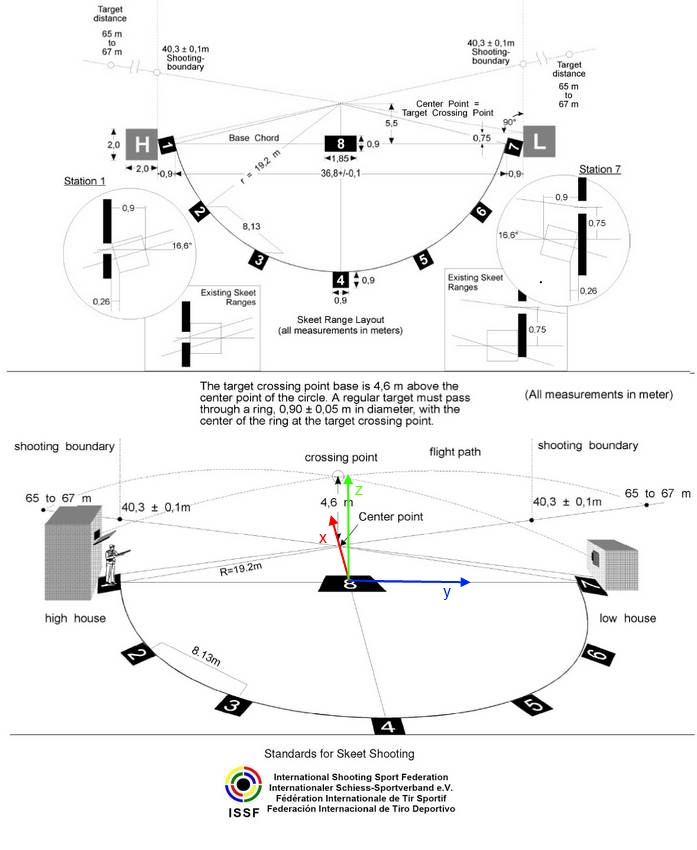
\includegraphics[width=0.4\textwidth]{./graphics/skeet-diagram_med_akser}
\caption[tekst i indholdsfortegnelsen]{figurtekst}
\label{fig:ES}
\end{figure}	
Systemets input er 60 kartesisiske koordinatsæt (x,y,z) per sekund. Hvor disse 
koordinater stammer fra, er uden for projektafgrænsningen. \\

Systemet dimensioneres til brug ifbm. en konkurrence i ES. En skitse over 
banen ses på figur \ref{fig:ES}. Det kartesiske koordinatsystem har origo i halvcirklens centrum, 
som indtegnet \todo[inline, author=Michael]{De er så indtegnet forkert.. Flot arbejde, klaphat..} 
nederst på figuren. I ES skal rammes serier af duer/mål der afskydes fra 
enten ”High House” eller ”Low House”, og med skud fra hver af de otte stationer langs 
cirkelperiferien. I dette projekt kigges kun på tilfældet hvor der afskydes mål fra ”High-
House” med pan-and-tilt systemet placeret på station 4.\\

Jævnfør reglerne for ES, skal duer/mål passere target crossing point (TCS) som er 
placeret i $4,57 [m]$ over origo. (0; 0; 4.57). Fejlmargin for passagen er $\pm0,45 [m]$. 
Målene skal desuden flyve $50 – 52 [m]$.  High house er placeret $20,11 [m]$ fra TCS, i en 
højde af $3,05 [m]$. Da luftmodstanden er negligerbar kan parablen (2. grads 
polynomium) findes ved at indsætte de kendte punkter. Herunder er parablen vist i et 
2D plan, figur \ref{fig:HH2D_para}.
\begin{figure}[!th]
\centering
\begin{tikzpicture}[scale=1]
\include*{./graphics/high_house_2D_parabola}
\end{tikzpicture}
\caption[Lerdue parabel]{Viser parablen af lerduens bane.}
\label{fig:HH2D_para}
\end{figure}
\todo[inline, author=Anders]{Den rigtige funktion skal sættes ind, afventer Michael}




Målet bliver affyret med en hastighed på $34 [m/s]$, i en vinkel på $9^{\circ}$ ift. xy-
planet. Set ovenfra bevæger målet sig som set på figur \ref{fig:para_in_xy_plane}. 
Figuren ses nedslagspunktet fra High-House, der er i alt $52 [m]$ startpositionen samt 
PTS placering i punktet B. 



\begin{figure}[!th]
\centering
\begin{tikzpicture}[scale=1]
\include*{./graphics/parabola_in_xy_plane}
\end{tikzpicture}
\caption[tekst i indholdsfortegnelsen]{figurtekst}
\label{fig:para_in_xy_plane}
\end{figure}

\todo[inline, author=Anders]{Jeg er gået igang med at tegne den og den kommer in snart.}

\subsection{Udregning af tallene}
\todo[inline, author=Michael]{Skal sikkert flyttes til appendix, hvis ikke det skal droppes helt? Bare så i kan se hvad jeg har haft gang i.}

For at simplificere udregningerne, regnes parablen kun i 2D. Det er trivielt at tilføje den tredje, så det gøres til sidst (hvis jeg finder det relevant). 

Kasteparablen er givet ved vektorfunktionen i ligning  \ref{eq:pf:vektorparabel}.

\begin{equation}
	Pos(t) = \left( \begin{array}{c}
	x(t) \\
	y(t)
	\end{array}
	\right)
	= \left( \begin{array}{c}
	\cos \theta v_0 t + x_0 \\
	\sin \theta v_0 t - \frac{g}{2} t^2 + y_0
	\end{array}
	\right)
\label{eq:pf:vektorparabel}
\end{equation}

Hvor $\theta$ er afskydningsvinklen, $v_0$ er afskydningshastigheden, $g$ er tyngdeacceleration og $x_0$,$y_0$ er begyndelsespunktet. 

For at få en parabel på formen y(x), isoleres t i x(t) med henblik på at substituere t i y(x): ($x_0$ sættes til 0.)

\begin{equation}
t = \frac{x}{\cos \theta v_0}
\label{eq:pf:x(t)}
\end{equation}

Den fundne værdi for t indsættes i $y(t)$, og udtrykket reduceres: 

\begin{eqnarray}
y(t(x)) &=& \sin \theta \frac{x}{\cos \theta v_0} v_0 - \frac{g}{2} \left(\frac{x}{\cos \theta v_0}\right)^2 + y_0 \\
y(x) &=& \tan \theta x - \frac{gx^2}{2(\cos \theta v_0)^2} + y_0
\label{eq:pf:y(x(t))}
\end{eqnarray}

Det ses at der er 3 ubekendte i ligningen. Dog er 3 punkter kendt fra HH parablen. Det er givet i reglerne for ESS at målet affyres fra en højde på 3.05 [m], så det indsættes i formlen. 
\begin{equation}
y(x) = \tan \theta x - \frac{gx^2}{2(\cos \theta v_0)^2} + 3.05
\label{eq:pf:y(x)2}
\end{equation}
Det er givet at målet skal passere TCS som er placeret i en højde på 4.57 [m], 20.11 [m] fra HH. 
Desuden skal målet bevæge sig 50 - 52 [m], i de videre beregninger 52 [m]. Det giver koordinatsættene (20.11; 4.57) og (52; 0). Vha. disse bestemmes $\theta$ og $v_0$ til:\footnote{Ved g = 9.82}
\todo[inline, author=Michael]{Måske giver det ikke mening med alle de decimaler, da det er udregnet med g = 9.82 - men jeg ved heller ikke hvor jeg skal finde en mere præcis måling af g?}
\begin{eqnarray}
\theta &=& 9.103 \degree \\
v_0 &=& 34.589 \frac{m}{s}
\end{eqnarray}
Disse parametre indsættes i vektorfunktionen fra ligning \ref{eq:pf:vektorparabel} samt udtrykket fra ligning \ref{eq:pf:y(x)2} og giver: 
\begin{equation}
	Pos(t) = \left( \begin{array}{c}
	x(t) \\
	y(t)
	\end{array}
	\right)
	= \left( \begin{array}{c}
	\cos \left(9.103 \degree \right) 34.589 t \\
	\sin \left(9.103 \degree \right) 34.589 t - \frac{9.82}{2} t^2 + 3.05
	\end{array}
	\right)
\label{eq:pf:vektorparabel2}
\end{equation}

\begin{equation}
y(x) = \tan \left(9.103 \degree \right) x - \frac{9.82x^2}{2(\cos \left(9.103 \degree \right) 32.589)^2} + 3.05
\label{eq:pf:y(x)3}
\end{equation}
\section{Kravspecifikation}
\label{sec:kravspecifikation}
Kravene til systemet findes vha. reglerne for ES \citep{ES_regler}.

% Lerduens bane beregnes vha. de i reglerne givne værdier for affyringspunkt (D), forventet nedslagspunkt (G) og "target crossing point" (TCS).

I reglerne er givet et affyringspunkt (D), et forventet nedslagspunkt (G) og ``target crossing point'' (TCS).
%Med antagelsen om negligerbar luftmodstand kan en kasteparabel således udregnes ved interpolation af disse tre punkter.
Lerduens parabelbevægelse findes ved interpolation af disse tre punkter. Det antages at luftmodstanden er neglibar.
%Kasteparablen er givet ved ligning \ref{eq:ks:vektorparabel3d}, med origo som angivet på figur \ref{fig:ES}.
%\begin{equation}
%Pos\left( t \right) = 
%\left( \begin{matrix} 
%	x\left( t \right)  \\ 
%	y\left( t \right)  \\ 
%	z\left( t \right)  \end{matrix} \right) =
%	 \left( \begin{matrix} 
%	- 9,34\cdot t+5,5 \\
%  32,851\cdot t-19,3 \\ 
% -{ 4,91\cdot t }^{ 2 }+5,473\cdot t+3,05\end{matrix} \right) [\text{m}]
%\label{eq:ks:vektorparabel3d}
%\end{equation}

%Med kasteparablen er det muligt at specificere systemets betingelser yderligere:
%Lerduens affyringshastighed og vinkel ift. xy planet kan lerduens flugt beregnes. 
%
Lerduens affyringshastighed og vinkel ift. xy planet blev beregnet vha. den fundne kasteparabel. 
% Lerduen affyres med en hastighed på 34,589 \([\frac{m}{s}]\) i en vinkel på \(9,103 \degree\) 
Lerduen affyres med en hastighed på 34,6 \([\frac{m}{s}]\) i en vinkel på \(9,1 \degree\) 
ift. xy-planet jf. figur \ref{fig:ES}\footnote{Beregningerne bag kasteparablen findes i appendix \ref{sec:udregning_af_parabel}.}. 

Lerduens flugt er givet i ligning \ref{eq:ks:vektorparabel3d} med origo som angivet på figur \ref{fig:ES}. 

\begin{equation}
Pos\left( t \right) = 
\left( \begin{matrix} 
	x\left( t \right)  \\ 
	y\left( t \right)  \\ 
	z\left( t \right)  \end{matrix} \right) =
	 \left( \begin{matrix} 
	- 9,34\cdot t+5,5 \\
  32,851\cdot t-19,3 \\ 
 -{ 4,91\cdot t }^{ 2 }+5,473\cdot t+3,05\end{matrix} \right) [\text{m}]
\label{eq:ks:vektorparabel3d}
\end{equation}
%En gennemgang af beregningerne der ligger bag kasteparablen findes i appendix \ref{sec:udregning_af_parabel}.

Lerduens flugt er illustreret på figur \ref{fig:para_total}.
Punktet D er "high house".
Punktet SB og punktet G er hhv. 40,3 [m] og 52 [m] fra "high house". \\
\begin{figure}[h!]
\centering
\subfloat[Lerduens højde som funktion af afstanden langs xy-planet.\label{fig:HH2D_para}]{%
	\begin{tikzpicture}[scale=0.8]
	\include*{./graphics/high_house_2D_parabola}
	\end{tikzpicture}
}
\subfloat[Lerduens bane projekteret på xy-planet.\label{fig:para_in_xy_plane}]{%
	\begin{tikzpicture}[scale=0.16]
	\include*{./graphics/parabola_in_xy_plane}
	\end{tikzpicture}
}
\caption[Lerduens parabel i 2D]{Viser lerduens parabelbevægelse i 2D.}
\label{fig:para_total}
\end{figure}

Tilt-rammen kan bevæge sig frit,
men pan-rammen kan pga. en stopklods ikke rotere frit.
Bevægelsesområdet er målt til \(154 \degree\).

Haglene fra et 12 gauge haglgevær med Skeet Choke spredes så de dækker et område
%med en diameter på 1,32 [m] på en afstand til centrum af cirklen på 37 [m] 
med en diameter på 1,32 [m] på 37 meters afstand
\citep[Pattern and choke]{patternandchoke}.
Spredningsvinklen er, med en antagelse om lineær spredning, givet ved ligning \ref{eq:ks:spredning}.
\begin{align}
\begin{split}
  Spredning &= 2\cdot{}\tan^{-1}\left(\frac{1,32/2}{37}\right) \\
  &= 2,04 \degree
  \end{split}
  \label{eq:ks:spredning}
\end{align}
%Der er altså et krav om at geværet peger på lerduen med en præcision på \(\pm 1,02 \degree\).
Når trackingfejlen defineres ud fra pan-vinklen \(\theta\) og tilt-vinklen \(\phi\) som i ligning \ref{eq:ks:trackingerror} rammes 
lerduen ved afskydning af haglgeværet når ligning \ref{eq:trackingerrorkrav} opfyldes.
\begin{align}
  TE = \left | \begin{pmatrix}  \theta_{\text{target}}\\ \phi_{\text{target}}\end{pmatrix} - \begin{pmatrix} \theta_{current}\\ 
  \phi_{current}\end{pmatrix} \right | &&\text{(Trackingfejl)}
\label{eq:ks:trackingerror}
\\
	TE\leq 1,02 \degree && \text{(Lerduen rammes)}
\label{eq:trackingerrorkrav}
\end{align}

Settling Time defineres som tiden der går før trackingfejlen forbliver \(\leq 1.02 \degree\).
%som skrevet i ligning \ref{eq:ks:settlingtime}.
%\begin{align}
%{ { t }_{ s }\quad =\left t \right|  }_{ TE\leq 1,02 \degree }
%\label{eq:ks:settlingtime}
%\end{align}

Der skydes på lerduen mellem toppunktet og SB.
I dette tidsrum skal PTS sigte præcist på lerduen under opfyldelse af ligning \ref{eq:trackingerrorkrav} og dette 
stiller krav til Settling Time, \(t_s\), som skrevet i ligning \ref{eq:ks:settlingtime1}.
%Tidspunktet, hvor lerduen når sit toppunkt er altså samtidigt tid er altså det højeste settling time må være, ligning \ref{eq:ks:settlingtime1}

\begin{align}
  t_{top} &= 0,557\text{ [s]} &\text{(Toppunktet af parablen)}
  \label{eq:ks:toppunktstid}
  \\
  t_{s} & \leq 0,557\text{ [s]} &\text{(Krav til Settling Time)}
  \label{eq:ks:settlingtime1}
  \\
   t_{SB} &= 1,180 \text{ [s]} &\text{(SB)}
  \label{eq:ks:sbtid}
\end{align}

%I dette tidsrum skal Pan \& Tilt-systemet sigte præcist på lerduen og kravet til 
%tracking error i ligning \ref{eq:ks:trackingerrorsize} skal overholdes.
%Der er altså et tidsmæssigt krav til reguleringen om en indsvingningstid (Settling Time) for systemet,
%der er lavere end tiden \(t_{s}\) angivet i ligning, \ref{eq:ks:settlingtime}.
%Dette krav gælder for både pan-rammens vinkel (\(\phi\)) og tilt-rammens vinkel (\(\theta\)).
%For en 1-radian reference giver dette altså en maksimal trackingerror (SSE) på 1,78\%.
%\todo[inline, author=Michael]{Den virkelige sammenhænge er mere kompleks: Hvis både pan \& tilt rammen peger 1\degree ved siden af, er den samlede afvigelse vel over 1,02\degree}
%\todo[inline, color = pink, author = Mikkel]{Hvad mening giver det at kigge på 1 radian reference og kan man virkelig kalde det SSE?}
Det eneste krav der stilles til systemet er Settling Time kravet beskrevet i ligning \ref{eq:ks:settlingtime1}.

%Dette giver altså en øvre og en nedre grænse for pan-rammens maksimale udsving,
%som afhænger af reguleringen
%- et for højt overshoot på pan-positionen kan give udsving, der ikke holder sig inden for grænserne.
%Hvis det antages, at vinklen \(0 \degree\) er lige midt imellem pan-rammens rotationsgrænser,
%så den kan rotere \(77 \degree\) til hver side, så er det maksimale overshoot for et 1-radians step-input
%givet ved \(34 \%\).
%\todo[inline, color = pink, author = Mikkel]{Hvad mening giver den 1 radian reference?}
%\todo[inline, author=Michael]{Indsæt evt. figur med overshoot begrænsninger?}



\section{Projektoverblik}
\label{sec:projektoverblik}
Som det fremgår af projektoplægget skal projektet opdeles som vist på 
figur \ref{fig:overview_openloop_PTS}. 
Det ligger altså udenfor dette projekt at bestemme den overordnede opdeling.
Projektoplægget stiller ydermere følgende krav til implementeringen:
\begin{itemize}
\itemsep1pt
  \item Regulatorerne skal implementeres på én mikroprocessor.
  \item Der skal benyttes SPI kommunikation mellem mikroprocessoren og FPGA’en.
  \item FPGA’en skal styre PWM-signalerne til motorerne.
  \item FPGA’en skal benyttes til bestemmelse af motorernes position vha. encoderne.
\end{itemize}

\bigskip

\begin{figure}[!th]
\centering
\begin{tikzpicture}[auto, node distance=1cm,>=latex']
\include*{./graphics/PTSoverview}
\end{tikzpicture}
\caption[Principskitse af PTS]{Principskitse af PTS.}
\label{fig:overview_openloop_PTS}
\end{figure}


% Følgende er blot gentagelser. 

%De grønne kasser på figur \ref{fig:overview_openloop_PTS}
%repræsenterer mikrocontrolleren som vha. UART kommunikerer med brugeren. \\
%FPGA'en er repræsenteret vha. en lilla kasse som er bindeledet mellem mikrocontrolleren og de to DC motorer. 
%FPGA'en og mikrocontrolleren kommunikerer sammen vha. SPI.
%FPGA'en genererer to PWM-signaler, som driver hhv. H-broen og motor for
%pan og H-broen og motor for tilt. DC-motorene sender deres encoder feedback til FPGA'en.
\part{System identifikation}
Denne del af rapporten beskriver hvordan systemet identificeres ved at finde en 
matematisk model for systemet. Dernæst findes de krav, det kræver at styre et 
sådant system. Der beskrives hvilken koordinattransformation der er behov for.
Ydermere beskrives hvilken proces, der benyttes til at designe regulatoren samt 
hvordan den matematiske model for systemet diskretiseres.

\section{PTS's inertimoment}
\label{sec:teo_PTS}

For at kunne modellere reguleringssløjerne bedst muligt er det essentielt at have de variable, 
som påvirkes fra PTS. Dette bevirker at der skal findes en teoritisk værdi for inertimomentet for den 
kvadratiske aluminiums ramme og et inertimoment for den u-formet aluminiums ramme, hhv. tilt og pan.\\
Figur \ref{fig:inerti_PTS} viser en skitse af systemet med opmålinger foretaget manuelt, hvor ${L_{1}} =0,292 [m]$,
${L_{2}} =0,280 [m]$, ${L_{3}}= 0,42 [m]$, ${L_{4}} =0,246 [m]$, ${L_{pro}}=0,04 [m]$.
\begin{figure}[!th]
\centering
\begin{tikzpicture}[scale=0.8]
\include*{./graphics/inerti_PTS}
\end{tikzpicture}
\caption[Skitse af PTS]{Viser en skitse af system, hvorpå de to inertimomenter findes for PTS.}
\label{fig:inerti_PTS}
\end{figure}

Det har været nødvendigt at foretage simplificeringer til bestemmelsen af PTS inertimoment. 
Idet vores viden kun har kendskab til SISO\footnote{Single input - single output.}-systemer, vil PTS anses som værende uafhængige strukturer.\todo[author=Anders,inline,color=gray! 100]{Mikael, her skal vi lige have snakket omkring, 
hvordan vægten for tilt skal påvirke pan. Tilt anses som værende symmetrisk omkring pan's 
rotation, derfor tænker jeg at tilts vægt bare skal lægges til ${L_{3}}$.} 

\subsection{Simplificering samt bestemmelse af PTS's inertimoment}
Den teoritiske beregning er foretaget ud fra følgende simplificeringer:
\begin{itemize}
\item Aluminimumsprofilen, 40x40L, har en massefylde på $\rho=1,5 [kg/m]$, \citep[Kap. 2 side. 4]{alu_profil_desitet}. 
\item Inertimomenterne for aluminimumsprofilerne ${L_{2}}$ og ${L_{4}}$ er bestemt udfra punktmasser, som er parallelforskudt i forhold til rotationsaksen. \citep[Side. 254, ligning 10-36]{fund_of_physics}.
\begin{equation}
I={ I }_{ com }+M\cdot { h }^{ 2 }
\label{eq:punktmasse_para} 
\end{equation}
hvor ${I_{com}} = 0$ og $h$ er afstand til punktmassen fra rotationsaksen.
\item Inertimomenterne for aluminimumsprofilerne ${L_{1}}$ og ${L_{3}}$ er bestemt som en tynd stang, hvor stagens center er placeret vinkelret på rotationsaksen. \citep[Side. 255, tabel 10-2e]{fund_of_physics}.
\begin{equation}
I=\frac { 1 }{ 12 } M\cdot { L }^{ 2 }
\label{eq:punktmasse_para} 
\end{equation}
\end{itemize}

Med følgende bestemmelser er det muligt at finde pan og tilts teoritiske inertimoment.
\begin{align}
\label{eq:inerti_tilt_pan}
\begin{split}
{ inerti }_{ tilt } &= \left( \left( 1/12\cdot \rho \cdot { {L_{1}} }^{ 3 } \right) +\left( \rho \left( {L_{2}}-2\cdot {L_{pro}} \right) { \left( \frac { {L_{1}}-{L_{pro}}}{ 2 }  \right)  }^{ 2 } \right)  \right) \cdot 2
\\
{ inerti }_{ tilt } &= 0,0157499
\\
{ inerti }_{ pan }&=\left( 1/12\cdot \rho \cdot { { L }_{ 3 } }^{ 3 } \right) +\left( \rho \left( { L }_{ 4 }-{ L }_{ pro } \right) { \left( \frac { { L }_{ 3 }-{ L }_{ pro } }{ 2 }  \right)  }^{ 2 } \right) \cdot 2
\\
{ inerti }_{ pan } &=0,0315708
\end{split}
\end{align}

Inertimomenterne er beregnet i ligning \ref{eq:inerti_tilt_pan}. Dog skal gearingen mellem motorene og hhv. pan og tilt tages i betragtning. Set fra motorene er gearingsfaktoren 30:1, hvilket bevirker at det faktiske intermoment for hhv. pan- og tiltstrukturen er en tredive del mindre, ligning \ref{eq:inerti_tilt_pan_fak}.
\begin{align}
\label{eq:inerti_tilt_pan_fak}
\begin{split}
{inerti-fak}_{tilt}&=5,24997\cdot{10}^{-4} [kg \cdot {m}^{2}]
\\
{inerti-fak}_{pan}&=10,5236\cdot{10}^{-4} [kg \cdot {m}^{2}]
\end{split}
\end{align}

\subsection{Konklusion af PTS's inertimoment}
Ud fra simplificeringerne er inertimomentet for hhv. pan og tilt fundet. Selvom værdierne er små, tages de er betragtning til designet af de to kontrollere.




\section{Koordinattransformation}
\label{sec:koordinattransformation}

De kartesiske koordinater \(P_k=[x, y, z]\) skal transformeres til sværiske koordinater \(P_s=[\rho \text{ ; } \phi \text{ ; } \theta]\), hvor \(\phi\) og \(\theta\) bruges som vinkelbestemmelserne for hhv. tilt og pan og \(\rho\) er afstanden fra PTS til duen som funktion af tiden.
Positionbestemmelsen som funktion af tiden for det kartesiske koordinatset er udredt i afsnit \ref{subsubsec:para}.
Idet vinklerne skal bestemmes i forhold til PTS's rotationscenter og ikke koordinatsystemets origo, skal PTS's rotationscenter trækkes, \(PTS=[\text{0 ; 0,45 ; 19,2}]\). 
\subsection{Kartisk koordinater}
Koordinattransformation tager udgangspunkt i de kartisiske koordinater givet i ligning \ref{eq:pf:vektorparabel3d1}. 
\begin{align}
\begin{split}
{ P }_{ c }\left( t \right) &=Pos\left( t \right) -PTS
\\
&=\left( \begin{matrix} x\left( t \right) -0 \\ y\left( t \right) -0,45 \\ z\left( t \right) -19,2 \end{matrix} \right) 
\\ 
&=\left( \begin{matrix} 32,851\cdot t-19,2 \\ -{ 4,91\cdot t }^{ 2 }+5,473\cdot t+3,05-0,45 \\ 9,34\cdot t+5,5-19,2 \end{matrix} \right) 
\\
&=\left( \begin{matrix} 32,851\cdot t-19,2 \\ -{ 4,91\cdot t }^{ 2 }+5,473\cdot t+2,6 \\ 9,34\cdot t-13,7 \end{matrix} \right) 
\label{eq:pf:vektorparabel3d1}
\end{split}
\end{align}

Før koordinattransformationen fra kartesiske til sværiske koordinater vises et grafisk overblik af \(\phi\) og \(\theta\) samt \(\rho\), figur \ref{fig:thetaphi_degree}. Grundet PTS offset fra ligning \ref{eq:pf:vektorparabel3d1}, er origo for det særiske koordinatsystem, origo af PTS to rotationsakser. 

\begin{figure}[!th]
\centering
\begin{tikzpicture}[scale=4]
\include*{./graphics/3d_in_xyz_plane}
\end{tikzpicture}
\caption[Sværisk koordinatsystem til koordinattransformation]{Viser duens placering i det sværiske rum som funktion af  \(\phi\) og \(\theta\) samt \(\rho\).}
\label{fig:thetaphi_degree}
\end{figure}


\subsection{Sværisk koordinater}
Transformationen fra kartesiske koordinater til sværiske koordinater gøres ud for nedenstående ligning.
\begin{align}
\begin{split}
{ P }_{ s }\left( t \right) &=\left( \begin{matrix} \rho  \\ \phi  \\ \theta  \end{matrix} \right) =\left( \begin{matrix} \sqrt { { { P }_{ c_x }\left( t \right) }^{ 2 }+{ { P }_{ c_y }\left( t \right) }^{ 2 }+{ { P }_{ c_z }\left( t \right) }^{ 2 } }  \\ { tan }^{ -1 }\left( \frac { \sqrt { { { P }_{ c_x }\left( t \right) }^{ 2 }+{ { P }_{ c_y }\left( t \right) }^{ 2 } }  }{ { P }_{ c_z }\left( t \right) }  \right)  \\ { tan }^{ -1 }\left( \frac { { P }_{ c_y }\left( t \right) }{ { P }_{ c_x }\left( t \right) }  \right)  \end{matrix} \right) 
\\
 &=\left( \begin{matrix} \sqrt { { \left( 32,851\cdot t-19,2 \right)  }^{ 2 }+{ \left( -{ 4,91\cdot t }^{ 2 }+5,473\cdot t+2,6 \right)  }^{ 2 }+{ \left( 9,34\cdot t-13,7 \right)  }^{ 2 } }  \\ { tan }^{ -1 }\left( \frac { \sqrt { { \left( 32,851\cdot t-19,2 \right)  }^{ 2 }+{ \left( -{ 4,91\cdot t }^{ 2 }+5,473\cdot t+2,6 \right)  }^{ 2 } }  }{ 9,34\cdot t-13,7 }  \right)  \\ { tan }^{ -1 }\left( \frac { -{ 4,91\cdot t }^{ 2 }+5,473\cdot t+2,6 }{ 32,851\cdot t-19,2 }  \right)  \end{matrix} \right) 
\label{eq:sv_koordi}
\end{split}
\end{align}
hvor \(\rho\) er afstanden i meter, \(\phi\) og \(\theta\) er angivet i grader. \citep[Kap. 10.6, s. 598]{adam}.

\section{Regulator}
\label{sec:kontrollerdeign}
Det er valgt at designe regulatoren efter processen illustreret i figur \ref{fig:designproces}.
\begin{figure}[!th]
\centering
\include*{./graphics/designproces}
\caption[Designprocessen]{Designprocessen, \citep[Side. 260]{reg_modern_control_systems}.}
\label{fig:designproces}
\end{figure}

Formålet med reguleringen er som beskrevet i afsnit \ref{sec:problemformulering},
at kontrollere pan- og tilt-rammernes position, så de tracker en lerdue.
Dette gøres ved styring af deres hastighed, ved at justere spændingsfaldene over de
to DC-motorer. Spændingsfaldene styres af PWM-generatorer, og regulatoren
kan derfor styre motorernes hastighed ved at vælge PWM-signalernes duty cycles.

I afsnit \ref{sec:kravspecifikation} opstilles kravene til systemets respons.
Disse er for en 1-radian\todo[author=Anders]{Der bruges grader i resten af rapporten.} reference opsummeret nedenfor.
\begin{itemize}
\item \(t_{s} \leq 0,557 \mathrm{\left[s\right]}\) (Settling Time)
\item \(SSE \leq 1,78 \%\) (Steady State Tracking Error)
\item \(P.O. \leq 34 \%\) (Overshoot i procent)
\end{itemize}

Det er fastlagt i projektoplægget, at regulatoren skal implementeres på mikrocontrolleren.
Da systemet som input modtager kartesiske koordinater,
skal der også på mikrocontrolleren foregå en koordinattransformation
til den logiske vinkelrepræsentation med sfæriske koordinater.
Systemets konfiguration består altså af en koordinattransformation,
en regulering, en aktuering og en positionsmåling, som illustreret
i figur \ref{fig:digitalkontroller1}.
Bemærk at denne konfiguration er for ét SISO-undersystem (enten pan eller tilt),
og at mikrocontrolleren skal regulere begge SISO-undersystemer.
\begin{figure}[!th]
\centering
\begin{tikzpicture}[auto, node distance=2.6cm,>=latex']
\include*{./graphics/digitalkontroller1}
\end{tikzpicture}
\caption[Systemkonfiguration]{Systemkonfiguration (blokdiagram).
	Området markeret med stiplet linje udgør den digitale regulator.
	De grønne ovaler angiver "clocksignaler", som leverer pulser til de digitale dele af systemet.}
\label{fig:digitalkontroller1}
\end{figure}
Som beskrevet i afsnit \ref{sec:problemformulering},
så er input-samplingen fastlagt til at foregå med en frekvens på 60 [Hz].
Men som illustreret på figur \ref{fig:digitalkontroller1}, så skal reguleringssløjfen
"køres" (sample) med en frekvens \(f_s=\frac{1}{T_s}\), der ikke nødvendigvis er 60 [Hz].
\todo[inline, color = pink, author = Mikkel]{Skal opdateres med den frekvens vi bliver enige om.}
Dvs. A/D- og D/A-konverteringerne (ikke input-samplingen) skal foregå med frekvensen \(f_s\).

Der er overordnet to strategier til valg af samplingfrekvensen \(f_s\) hvormed
reguleringssløjfen skal køre:
1) Hvis man designer en kontinuert regulator til det kontinuerte domæne, så
skal diskretiseringen af controlleren være så tæt på den kontinuerte regulator som muligt.
Det vil sige, samplingfrekvensen skal vælges så høj som mulig.
2) Hvis man derimod designer en diskret regulator til det diskrete domæne,
så er diskretiseringen allerede foretaget inden designet af regulatoren.
Dvs. man finder en diskretiseret model af det fysiske system inden designet af regulatoren.
Kravet til diskretiseringen af åbensløjfeoverføringsfunktionerne er, at den diskrete repræsentation
skal være tilfredsstillende tæt på de kontinuerte overføringsfunktioner.
Hvis den diskrete overføringsfunktion eksempelvis afviger 20 \% fra den kontinuerte, ville man
sandsynligvis overveje at benytte en højere samplingfrekvens til diskretiseringen.
Sammenligningen af den diskrete overførselsfunktion og den kontinuerte overføringsfunktion
kan være både i tidsdomænet (fx steprespons) og i frekvensdomænet (frekvensrespons, fx. Bode-plots).
Når man har den diskretiserede model af systemet, kan man i det diskrete domæne (z-domænet)
udvikle en regulator - denne er altså diskret fra starten.

Da reguleringen foregår i en task på mikrocontrolleren, vælges det
at udvikle en diskret regulator efter en diskretiseret model af systemet.
Således kan perioden hvormed regulerings-task'en skal køre, fastlægges ud fra
samplingperioden \(T_s\). Hvis man havde valgt at designe en kontinuert regulator
ville perioden skulle vælges så lav som muligt, og dette ville stille højere krav
til mikrocontrolleren.

\subsection{Diskretisering af åbensløjfeoverføringsfunktionerne}
Som beskrevet ovenfor ønskes det at finde en diskretiseret overføringsfunktion
for det fysiske system. Den kontinuerte del af systemet, som ønskes diskretiseret,
er markeret på figur \ref{fig:digitalkontroller2}.
\begin{figure}[!th]
\centering
\begin{tikzpicture}[auto, node distance=2.6cm,>=latex']
\include*{./graphics/digitalkontroller2}
\end{tikzpicture}
\caption[Diskretisering af åbensløjfeoverføringsfunktion]{Diskretisering af åbensløjfdeoverføringsfunktion.
	Den kontinuerte del af systemet (markeret med stiplet linje) ønskes diskretiseret.
	De grønne ovaler angiver "clocksignaler", som leverer pulser til de digitale dele af systemet.}
\label{fig:digitalkontroller2}
\end{figure}

Den diskretiserede åbensløjfeoverføringsfunktion fra duty cycle til output vinkel
benævnes \(G_{zoh}\left(s\right)\). Dette er fordi D/A-konverteringen modelleres som et Zero-Order Hold kredsløb,
der fastholder en analog værdi proportional med duty cyclen. Dette stemmer overens med den simplificerede
model for PWM-signalet beskrevet i afsnit \ref{subsec:matFPGA}.
Den diskrete overføringsfunktions plads i blokdiagrammet for systemet
er indtegnet i figur \ref{fig:digitalkontroller3}.
\begin{figure}[!th]
\centering
\begin{tikzpicture}[auto, node distance=2.6cm,>=latex']
\include*{./graphics/digitalkontroller3}
\end{tikzpicture}
\caption[tekst i indholdsfortegnelsen]{figurtekst}
\label{fig:digitalkontroller3}
\end{figure}
De to overføringsfunktioner hhv. \(G_{pan}\left(s\right)\) og \(G_{tilt}\left(s\right)\)
har hver en diskretiseret overføringsfunktion hhv. \(G_{zoh,pan}\left(z\right)\) og \(G_{zoh,tilt}\left(z\right)\).

Kravet til \(G_{zoh,pan}\left(z\right)\) og \(G_{zoh,tilt}\left(z\right)\) er, at de
med god tilnærmelse opfører sig som \(G_{pan}\left(s\right)\) og \(G_{tilt}\left(s\right)\),
og dette krav kan skrives som et mindstekrav til samplingfrekvensen \(f_s\).

\subsubsection{Valg af samplingfrekvens}
\label{subsec:choosefs}
Reguleringssløjfen skal køre periodisk på mikroprocessoren
med samplingfrekvensen \(f_s\). Denne skal vælges
ud fra systemets dynamik (til diskretiseringen), som beskrevet ovenfor,
fra samplingteoremet (Nyquist-frekvensen) samt ud fra
mikrocontrollerens begrænsninger.

Da samplingen af inputparablen (A/D-konverteringen) foregår fast ved 60 [Hz],
som beskrevet i problemformuleringen, er rekonstruktionen
af det oprindelige signal allerede her begrænset. Dvs. man
ikke kan få mere information om det oprindelige signal
uanset hvor hurtigt man sampler efter A/D-konverteringen af
det oprindelige signal.
Samplingfrekvensen på 60 [Hz] fortæller os,
at det oprindelige signal kun er bevaret op til 30 [Hz].
Hvis reguleringssløjfen køres med en frekvens på under 60 [Hz]
vil \textit{mere} information gå tabt.
Derfor skal reguleringssløjfen, ud fra samplingteoremet, helst køres
ved minimum 60 [Hz].

Diskretiseringen af åbensløjfeoverføringsfunktionerne stiller også krav til samplingfrekvensen.
Diskretiseringen skal altså sammenlignes med den kontinuerte overføringsfunktion.
Det vælges at sammenligne diskretiseringen af det fysiske system med det kontinuerte system i tidsdomænet.
Sløjfen lukkes med en forstærkning på 1, og step-responsens karakteristik sammenlignes
for den diskretiserede overføringsfunktion \(\frac{G_{zoh,tilt}}{1+G_{zoh,tilt}}\)
og for den kontinuerte overføringsfunktion \(\frac{G_{tilt}}{1+G_{tilt}}\) (en tilsvarende sammenligning foretages for pan).
Diskretiseringen opfører sig med bedste tilnærmelse som det kontinuerte system
når Rise Time, Settling Time og Overshoot efter diskretiseringen
ændrer sig så lidt som muligt i forhold til responsen af det kontinuerte system.
Det vurderes, at Rise Time og Settling Time maks. må ændre sig med 5 \% i forhold
til den kontinuerte respons, mens at Overshoot maks. må ændre sig med 25 \% i forhold til
den kontinuerte respons.
Dvs. det kan tolereres hvis overshoot
ved diskretiseringen ændrer sig fra 2 \% til 3 \%.

Hvis diskretiseringen kræver at reguleringssløjfen kører ved en frekvens \(f_s\),
der er højere end A/D-konverteringens 60 [Hz], skal det A/D-konverterede
signal "upsamples" til \(f_s\), og de spejlede "images" af sprektet ved \(n\cdot{}60 \mathrm{\left[Hz\right]}\) skal filtreres væk.
Upsamplingen har den simpleste implementering
hvis \(f_s\) er et heltalsmultiplum af den første samplings frekvens (60 [Hz])\todo[author=Anders]{eventuelt: frekvens på 60 [Hz].} \citep{dsp}\todo[author=Anders]{Konkret side i henvisningen.}.
Diskretiseringen af det fysiske systems åbensløjfeoverføringsfunktioner skal altså samples ved et heltalsmultiplum \(f_s\) af 60 [Hz].

På figur \ref{fig:diskretTiltStep} er stepresponsen for lukketsløjfesystemet (med forstærkning 1)
med \(G_{tilt}\) indtegnet sammen med den tilsvarende steprespons for to forskellige diskretiseringer
af \(G_{tilt}\). Som det ses af grafen, er det diskretiserede systems respons tættest
på det kontinuerte systems respons når samplingfrekvensen er højest.
\begin{figure}[!th]
\centering
	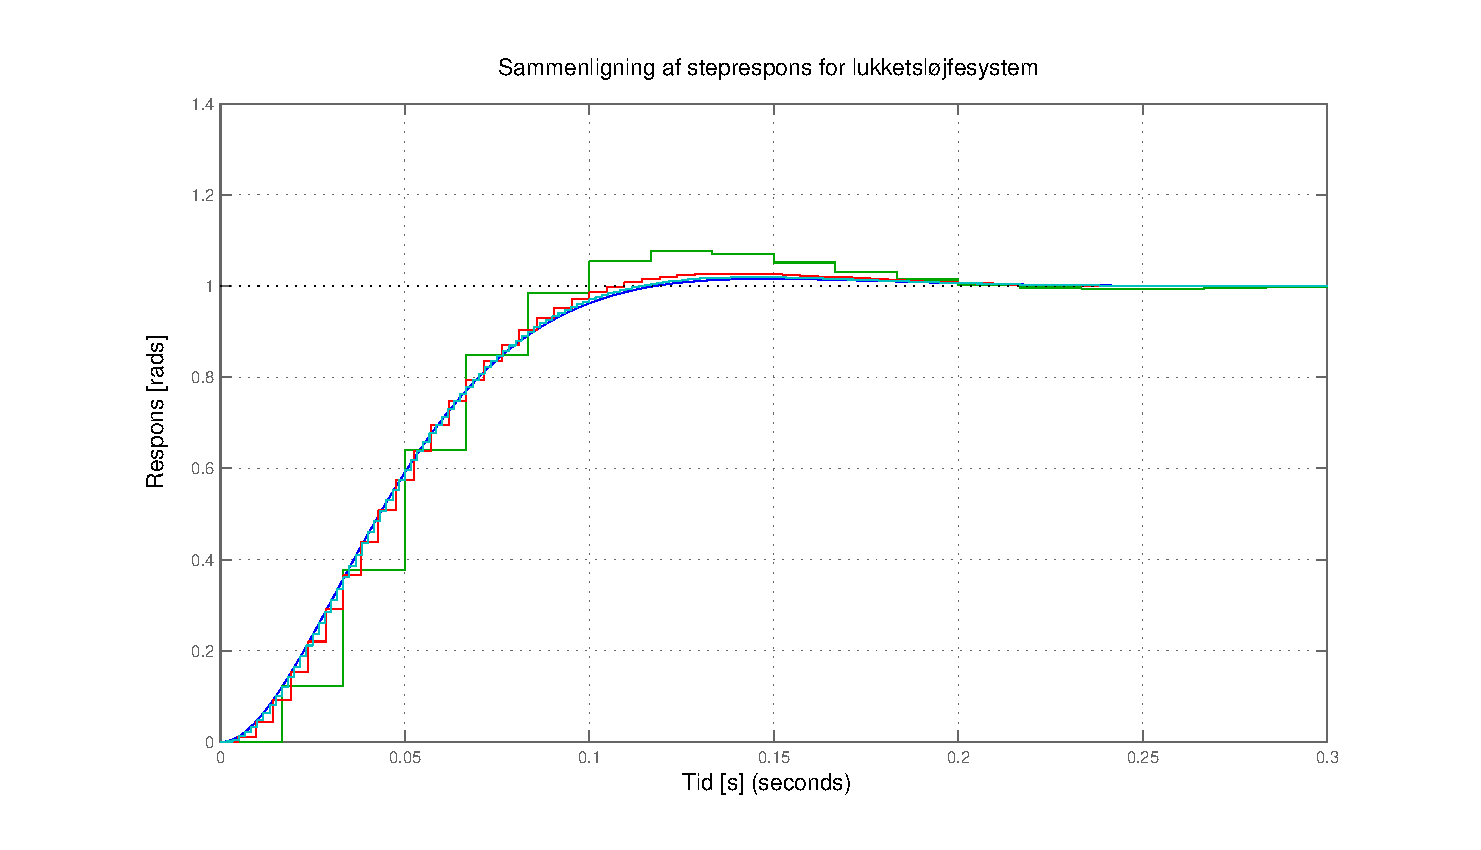
\includegraphics[width=1\textwidth]{./graphics/diskretTiltStep.eps}
\caption[Sammenligning af steprespons for kontinuert system med diskretiseret system]
{Sammenligning af steprespons for kontinuert system med diskretiseret system.
Den mørkeblå kurve er det kontinuerte systems respons,
og de andre kurver er det diskretiserede systems respons ved en samplingfrekvens på
60 [Hz] (grøn), 210 [Hz] (rød) og 600 [Hz] (lyseblå).}
\label{fig:diskretTiltStep}
\end{figure}
\todo[inline,author=Anders]{Der står både [s] og [seconds], den ene burde være nok.}
På figur \ref{fig:diskretStepFreq} er samme steprespons' performance afbildet
for pan og for tilt som funktion af samplingfrekvensen \(f_s\).
De sammenlignede størrelser er Rise Time, Settling Time og Overshoot.
Graferne viser ændringen af de tre størrelser i procent i forhold til det kontinuerte systems respons.
\begin{figure}[!th]
\centering
	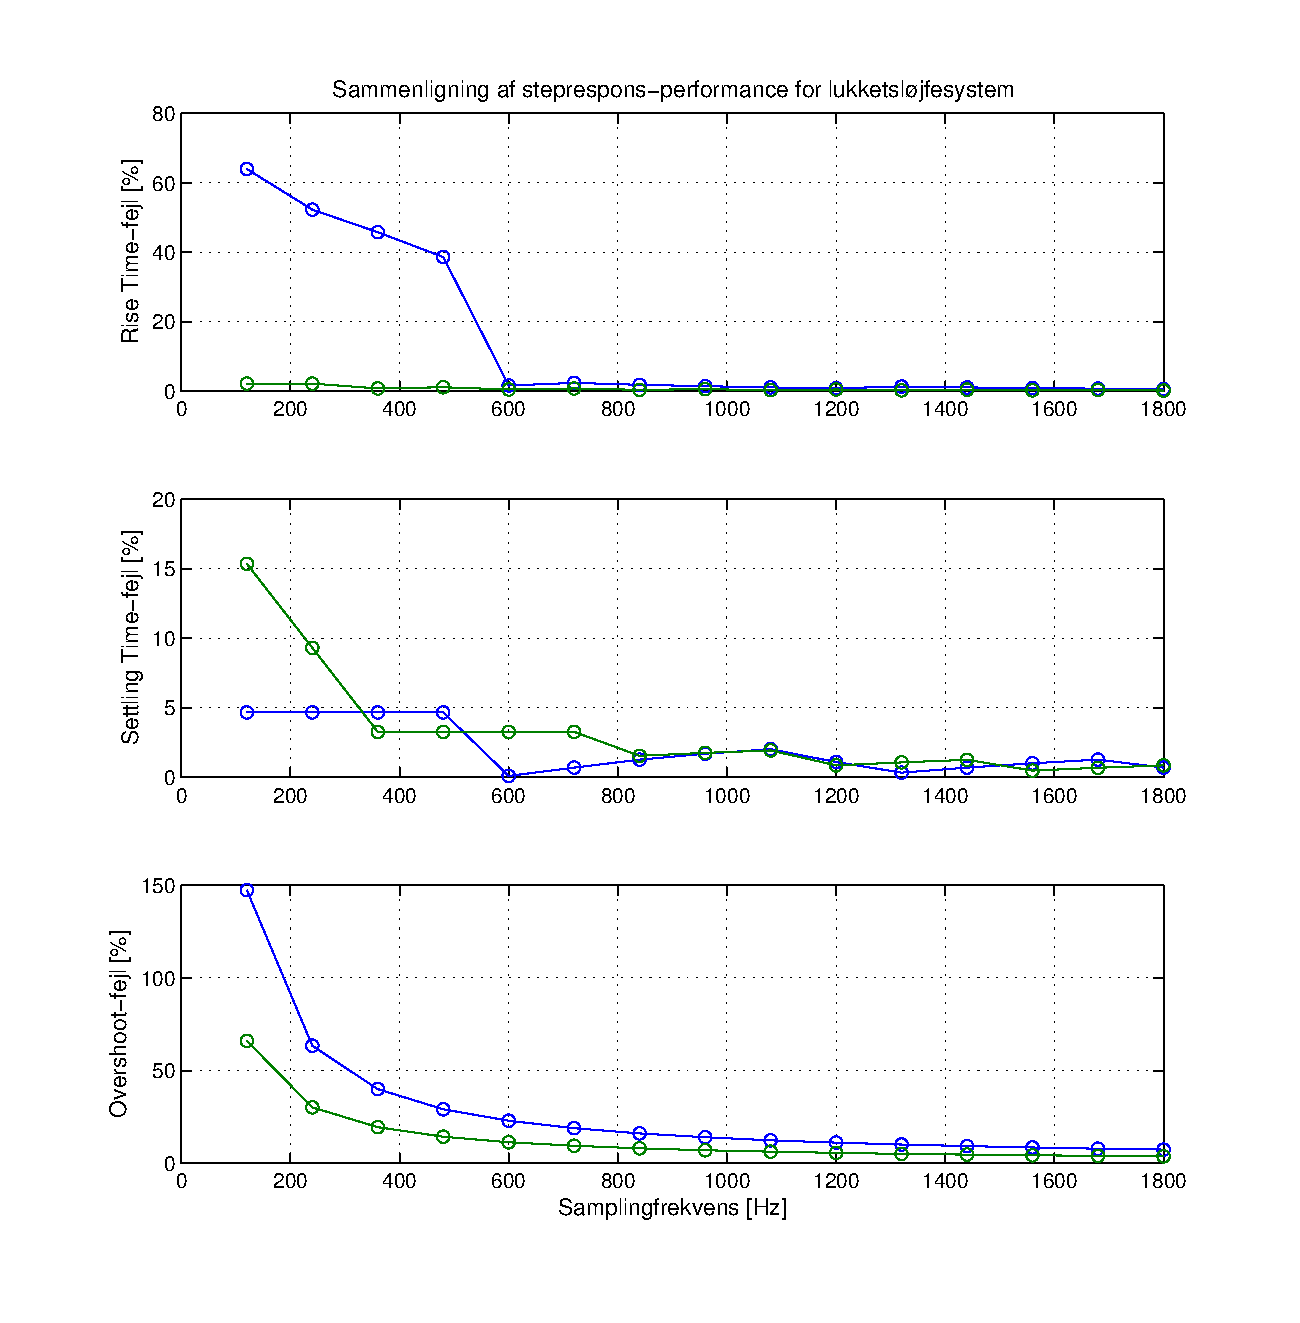
\includegraphics[width=1\textwidth]{./graphics/diskretStepFreq.eps}
%\caption[Sammenligning af steprespons-performance for kontinuert system med diskretiseret system (\(G_{zoh}\))]
%{Sammenligning af steprespons-performance for kontinuert system med diskretiseret system.
%Den blå kurve angiver fejlen i forhold til lukketsløjferesponsen af \(G_{tilt}\),
%mens den grønne kurve angiver fejlen i forhold til lukketsløjferesponsen af \(G_{pan}\).
%}

\caption[Sammenligning af steprespons-performance for kontinuert system med diskretiseret system $G_{zoh}$]
{Sammenligning af steprespons-performance for kontinuert system med diskretiseret system.
Den blå kurve angiver fejlen i forhold til lukketsløjferesponsen af $G_{tilt}$,
mens den grønne kurve angiver fejlen i forhold til lukketsløjferesponsen af $G_{pan}$.
}

% Åses LateX kan ikke lide \math\ i todo, caption og tilsvarende.

\label{fig:diskretStepFreq}
\end{figure}

Som forventet kan et generelt mønster ses på graferne i figur \ref{fig:diskretTiltStep} og figur \ref{fig:diskretStepFreq}:
Jo højere samplingfrekvens, jo tættere kommer diskretiseringens respons på det kontinuerte systems respons.
En yderligere inspicering viser, at en særligt god performance opnås ved en samplingfrekvens på 600 [Hz],
hvor kravene til diskretiseringens performance opfyldes.

Figur \ref{fig:diskretTiltStep} og figur \ref{fig:diskretStepFreq}
giver et grundlag for valg af reguleringssløjfens samplingfrekvens ud fra det fysiske systems dynamik.
Hvis mikrocontrollerens begrænsninger tages med i betragtning vil man vælge den lavest acceptable
samplingfrekvens af to årsager. Den ene årsag er, at jo højere periode, jo mindre CPU-belastning er der,
og jo mere tid er der til mikrocontrollerens andre opgaver som fx kommunikation med en PC-terminal.
Den anden årsag er, at reguleringssløjfen får mere tid til sine egne opgaver:
Koordinattransformation, upsampling, regulering (behandling af fejlsignalet) og SPI-kommunikation skal alt sammen foregå
inden for perioden \(\frac{1}{f_s}\).

Som udgangspunkt vælges derfor en samplingfrekvens på \(f_s=600 \mathrm{\left[Hz\right]}\),
så diskretiseringen med god tilnærmelse har samme performance som det kontinuerte system,
og så der er mest tid til reguleringssløjfens beregninger og SPI-kommunikation.

\subsection{Analyse af den diskretiserede}
\todo[inline,author=Anders]{Pan og tilt diskretiserende transferfunktioner. }

\begin{equation}
	pan
	\label{eq:pantiltdiskretiserendetf} 
 \end{equation}
 
Den i afsnit \ref{subsec:choosefs} udførte sammenligning af det diskretiserede systems performance
med det kontinuerte systems performance viser,
at Rise Time stiger med 3,3 \% for pan og 0,10 \% for tilt,
Settling Time stiger med 0,48 \% for pan og 1,6 \% for tilt,
samt at Overshoot stiger med 11 \% for pan og 23 \% for tilt
ved lukketsløjfesystemet med en forstærkning på 1.
Diskretiseringen sammenlignes i frekvensdomænet med det kontinuerte system
i figur \ref{fig:diskretBode}, der viser Bode-plot for \(G_{pan}\) og \(G_{tilt}\) samt
deres diskretiseringer (ved 600 [Hz]) \(G_{zoh,pan}\) og \(G_{zoh,tilt}\).
\begin{figure}[!th]
\centering
	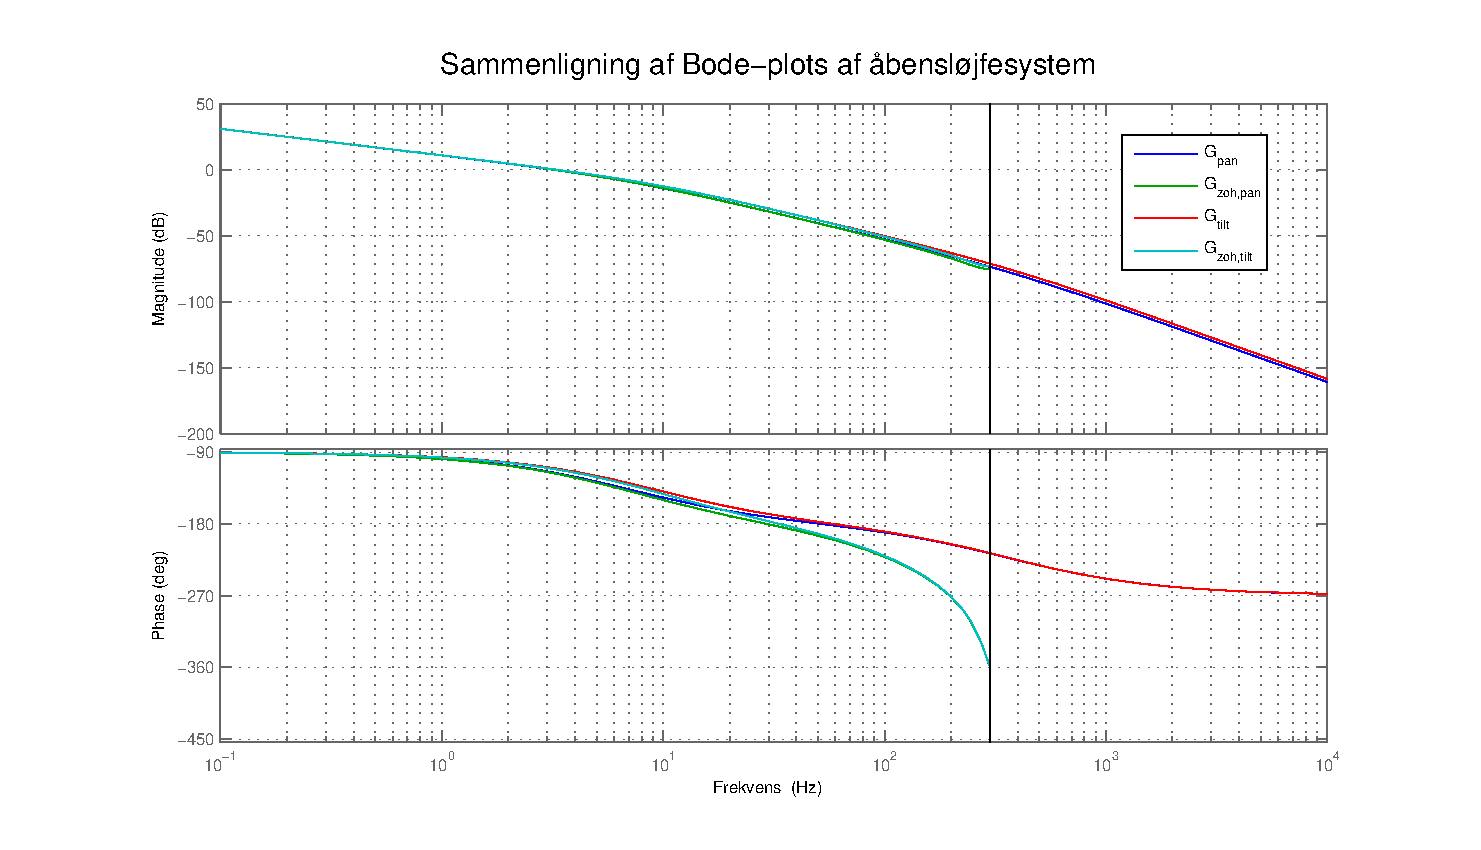
\includegraphics[width=1\textwidth]{./graphics/diskretBode.eps}
\caption[Sammenligning af Bode-plots af kontinuert system med diskretiseret system]
{Sammenligning af Bode-plots af kontinuert system med diskretiseret system.
Den blå og den røde kurve angiver hhv. \(G_{pan}\) og \(G_{tilt}\) mens
den grønne og den turkise kurve angiver hhv. \(G_{zoh,pan}\) og \(G_{zoh,tilt}\).
}
\label{fig:diskretBode}
\end{figure}
Bemærk at figur \ref{fig:diskretBode} er en sammenligning af \textit{åben}sløjfeoverføringsfunktionernes
frekvensrespons.

Som det ses på grafen, følger det diskretiserede systems respons meget nøje det kontinuerte systems respons.
Fejlen på størrelsen på responsen er meget lille i hele spektret,
mens fejlen på fasen er lille ved lave frekvenser og stiger ved høje frekvenser.

\subsection{Upsampling}
Da reguleringssløjfen, som beskrevet i afsnit \ref{subsec:choosefs}, køres med en frekvens på 600 [Hz],
som er 10 gange højere end input-samplingfrekvensen, skal der altså foretages en upsampling.
Upsamplingen indsætter mellem hvert input-sample 9 samples med værdien 0, så hvert input-sample
kun samples én gang. Dette gør, at input-signalets frekvensspektrum bevares.
Da input-signalet er samplet ved 60 [Hz] vil det oprindelige spektrum, centreret omkring 0 [Hz],
spejles ved heltalsmultipla af 60 [Hz]. Disse spejlbilleder af det oprindelige spektrum vil være
indeholdt i det upsamplede signal, hvis det ikke filtreres. Derfor skal et lavpasfilter anvendes,
som dæmper spejlbillederne af det oprindelige spektrum.

Kravene til lavpasfilteret er, at det med så få taps\todo[inline,author=Mikael]{Forklar taps}
som muligt skal give en rimelig dæmpning af
spejlbillederne af det oprindelige spektrum vedheltalsmultipla af 60 [Hz].

Det vælges at implementere et 21. ordens FIR-filter, da det foruden tilfredsstillende opfyldelse
af de ovennævnte krav også har lineær fase.
Da det meste af det oprindelige parabelspektrum findes ved 0 [Hz], vil det være
fordelagtigt at udnytte Gibbs-oscillationernes placering i frekvensspektret, således
at den højeste dæmpning er placeret ved heltalsmultipla af 60 [Hz].
\todo[inline,author=Mikael]{Indsæt to figurer:\\- Bode Plot af FIR-filter.\\- ufiltreret FFT vs. filtreret FFT}

\part{Implementering}
%Michael forsøger sig lige med en lille intro. 
Denne del af rapporten beskriver programmeringsmæssigt design og implementering af programmerne
på mikrocontrolleren og FPGA'en.
Der tages udgangspunkt i kravene til de enkelte dele der er opstillet i projektoplægget samt den foregående analyse af PTS.

Først beskrives designet, valg af skedulering,
implementering og test af programmet til mikrocontrolleren.
Dernæst beskrives implementeringen af de enkelte delelementer på FPGA'en.
\section{Mikrokontroller}
\label{sec:mikrokontroller}
\subsection{Krav til mikrokontrolleren}
Mikrokontrolleren har følgende opgaver: 
\todo[inline, author=Michael]{YOU CANT TOUCH THIS - lad mig lige skrive færdig!}
\begin{itemize}
	\item Afvikling af regulatorerne.
	\item Kommunikation med FPGA vha. SPI.
	\item Modtage kommandoer fra PC'en via UART.
	\item Sende relevant data til brugeren via UART.
\end{itemize}

Afvikling af regulatorerne skal afvikles i realtid, da det ellers er vanskelligt at modellere forsinkelsen. 


SPI\footnote{Serial Peripheral Interface, også kaldet SSI} bruges til at overføre PTS's position fra FPGA til mikrokontroller. Desuden overføres beregnet duty-cycle fra mikrokontroller til FPGA. Kommunikationen skal være tilpas hurtig, så regulatorerne ikke beregner på forældet data. 
\todo[inline, author=Michael]{Opstil bedre krav til SPI kommunikation, men hvordan? Det er vel noget med at den også skal reagere i realtid, så vi også kan modellere delayet fra SPI kommunikationen? Risiko for cirkelargumentation her. }

Systemet skal kunne modtage bruger inputs gennem et terminalprogram. Brugerinterfacet er ikke tidskritisk. Der skal være mulighed for at udlæse systemparametre:

\begin{itemize}
	\item PTS' position. 
	\item Ønsket position. 
	\item Log-fil.
\end{itemize}

Systemet skal reagere på følgende bruger inputs


\begin{itemize}
	\item Start tracking
	\item Stop tracking
	\item Reset systemet
	\item Gå til koordinat (x,y,z)
\end{itemize}


\subsection{Valg af skedulering}
Der er undersøgt 4 forskellige mulige skeduleringsalgoritmer: 

\begin{itemize}
	\item CoOS\footnote{coocox.com/CoOS.htm}
	\item freeRTOS\footnote{freertos.org}
	\item Run-To-Complete-Scheduler\footnote{Introduceret i EMP-kurset}
	\item Super-loop
\end{itemize}

Til valget er der lagt vægt på følgende parametre: 

\begin{itemize}
	\item Opfylder kravene til realtidsafvikling af regulatorerne. 
	\item Muligheden for at (gen)bruge elementer fra EMP-kurset.
\end{itemize}


\begin{tabular}{|l|l|l|l|l|}
\hline 
 & coOS & freeRTOS & RTCS & Super loop \\ 
\hline 
Skedulering & Preemptive  &   &   &   \\ 
									\\
\hline 
Indeholder queues &   &   &   &   \\ 
\hline 
Semaphorer og mutexes &   &   &   &   \\ 
\hline 
• & • & • & • & • \\ 
\hline 
\end{tabular} 


\subsection{Implementering}
\subsection{Test} 
\subsection{Delkonklusion}


\section{FPGA}
\label{sec:FPGA}
FPGA'en er leddet mellem mikrocontrolleren og motorene på PTS.
Følgende opgaver til FPGA'en er fastsat af projektbeskrivelsen:

\begin{itemize}
\itemsep1pt
	\item Kommunikation med mikrocontrolleren vha. SPI.
	\item Generering af PWM-signaler til motorerne på PTS.
	\item Optælling af motorernes rotationer vha. encoderne på PTS.
\end{itemize}
FPGA'en er i projeket et BASYS board\footnote{Datablad \citep{basys2}}, der programmeres ved brug af VHDL\footnote{VHSIC Hardware Description Language}.

\subsection{Valg i opbygning af FPGA funktionalitet}
Eftersom de fleste krav til FPGA'en er givet af projektbeskrivelsen, er der ikke 
lavet noget større analysearbejde af FPGA'ens funktionalitet. Undervejs i 
udviklingen af funktionaliteten er der dog taget nogle valg, som beskrives nedenfor.

\textbf{Generiske komponenter}\\
For at lave et system med lav kobling er det forsøgt at lave 
generiske komponenter til de funktionaliteter, der er af generel art. 
Til varetagelse af den resterende funktionalitet er der skrevet applikationsspecifikke 
komponenter.
Dette sikrer at koden er let at udbygge og genbruge.

\textbf{PWM}\\
Der skal fra FPGA'en genereres PWM-signaler til styring af motorerne på PTS.
Det ønskes at have en PWM-frekvens, der ikke ligger i det hørbare område, hvilket ca. går op til 20 [kHz]\citep{Hearingrange}. 
Det ønskes at have en opløsning på PWM, der er mindst ligeså høj, som 
opløsningen på PTS's positionsencodere, for ikke at forringe opløsningen på reguleringen. 
Det er derfor valgt at repræsentere PWM duty cycle med 11 bit. 
Ved 11 bits opløsning på PWM og brug af BASYS boardets interne clock på 50 [MHz] bliver PWM-frekvensen,
ligning \ref{eq:pwmfreq}, over det hørbare frekvensområde.

\begin{equation}
  f_{PWM}=\frac{50 \text{ [MHz]}}{2^{11}} = 24,41 \text{ [kHz]}
	\label{eq:pwmfreq}
\end{equation}

\textbf{Kalibrering af motorposition}\\
PTS skal kunne tændes i en tilfældig position og derefter kalibreres.
Kalibreringen af motorpositionen kan laves ved at sørge for at PTS drejer forbi 
de to hall sensorer, der er placeret på systemet. Dette vil give et signal, da 
der på PTS er placeret en magnet på hver af rammerne.
%Det blev besluttet at placere ansvaret for at dreje rammerne hen til hall 
%sensorerne hos mikrocontrolleren. Det blev besluttet, da det giver mulighed for 
%en simplere protokol mellem FPGA og mikrokontroller. Det sikrer samtidigt at mikrocontrolleren 
%altid har kontrol over hvordan PTS bevæger sig.
Funktionaliteten der skal være på FPGA'en er at opfange outputtet fra 
hall sensorerne og nulstille den tilhørende position.
Dog viste det sig, at hall sensorernes output ikke kun er højt på ét encodertick, 
men derimod adskillige. Det er nødvendigt at FPGA'en tager højde for 
dette.

\subsection{Opbygningen på FPGA}
\todo[inline,author=Mikael]{Opbygning på FPGA... Det lyder lidt mærkeligt, gør det ikke? Foreslår vi finder en bedre overskrift.}
På figur \ref{fig:FPGA_blok} ses et simplificeret diagram over komponenterne på FPGA'en. 
De grønne bokse angiver komponenter på FPGA'en, mens de grå cirkler angiver, hvad der ikke ligger på 
FPGA'ens chip. Pilene imellem FPGA'ens komponenter angiver retningen af 
datastrømme. Diagrammet er simplificeret ved at vise to ens komponenter som én. 
F.eks. er der ikke én tick counter komponent på FPGA'en, men derimod to.
Herunder følger en forklaring på hvordan de tre krav til FPGA'en er opnået. For 
yderligere forklaring af komponenterne henvises til appendix 
\ref{sec:fpgaappendix}.

\begin{figure}[!th]
\centering
\begin{tikzpicture}[node distance = 5 cm,scale=1]
\include*{./graphics/FPGA_blok}
\end{tikzpicture}
\caption[Diagram over FPGA komponenter]{Simplificeret diagram over komponenterne på FPGA'en}
\label{fig:FPGA_blok}
\end{figure}
%\todo[author=Åse,inline]{Teksten over figuren kan uddybes, med at beskrive de vigtigeste komponenter. Mens kan teksten nedenunder komme i appendix.}
%\subsection{SPI}
%På FPGA'en er SPI'en to shift registre. SPI'en konvertere det serielle signal fra MOSI til at parallel signal. Det signal sendes videre til Input decoder, som deler det op i komposanter. Fra Output decoder får SPI signalet, den skal sende til mikrocontrolleren.

\subsection[Kommunikation]{Kommunikation med mikrocontrolleren vha. SPI.}
På FPGA'en er implementeret en SPI slave der modtager data fra 
mikrocontrolleren. Data føres, i komponenten SPI, fra MISO ind i FPGA'en og fra FPGA'en ud på 
MOSI. Til mikrocontrolleren sendes skiftevis motorposition fra pan og tilt.

\subsection{Producering af PWM signal til motorerne på PTS}
I PWM komponenten produceres PWM-signalerne på baggrund af duty cycle værdier modtaget via. SPI. 
PWM bliver produceret ved at tælle en tæller op fra 0 til 2047 med 50 MHz.
PWM udgangen sættes høj indtil tælleren når dutycycle værdien og sættes lav 
ellers. Hermed er der produceret et PWM med en frekvens på ca. 24 kHz.

\subsection{Optælling af motorernes rotationer vha. encoders på PTS}
Da encoderne på motorerne er quadrature,
er det muligt at bestemme både retning og tælle rotationer på motoren. 
Dette sker i komponenten tick counter der afhængigt af inputtet fra encoderne tæller positionen op eller 
ned.
Der tælles ned fra 0 til 1079 og op fra 1079 til 0.
Reset-signal modtages fra komponenten tick reset, første gang pan og/eller tilts magnet bevæger 
sig over hallsensorerne.

\subsection{Delkonklusion}
FPGA'en fungerer som simpel slave i SPI-overførselen med mikrocontrolleren.
FPGA'en holder styr på pan og tilts motorpositon samt producerer PWM-signalerne 
med en frekvens på ca. 24 [kHz] og en opløsning på 2048.
%\section{Kommunikation mellem mikrocontroller og FPGA}

\begin{figure}[!th]
\centering
\begin{tikzpicture}[scale=1]
\include*{./graphics/MISOMOSI}
\end{tikzpicture}
\caption[tekst i indholdsfortegnelsen]{figurtekst}
\label{fig:}
\end{figure}


Kommunikationen mellem Mikrocontolleren og FPGA’en foregår med SPI. SPI står for Serial Peripheral Interface. Det er en protokol hvor, der bliver overført data mellem en master og en eller flere slaver. Overførelsen sker med full duplex, så der bliver sendt data både fra masteren og slaven på samme tid. Opstillingen mellem en master og en slave kan ses på figur ??.

Der er fire kanaler mellem masteren og slaverne: Slave Select, Serial Clock (SCLK), MOSI og MISO. Slave Select bruges til at vælge hvilken slave, der skal overføres data med. Den kan også sammenlignes med en chip select. SCLK bruges som clock frekvens, den synkroniserer Salve Select, MOSI og MISO. MOSI står for Master Output Slave Input, det er dataet, master sender til slaven, ligeså er MISO Master Input Slave Output, som er dataet, master modtager fra slaven.
 

\subsection{Overvejelser og valg}
Der er gået mange overvejelser i hvordan SPI'en mellem Mikrocontrolleren og FPGA'en skal  opbygges.

Det blev vedtaget at Mikrocontrolleren var masteren og FPGA'en blev slaven, da FPGA'en helst skulle være så enkel som mulig.

Mikrocontrolleren har også indbygget tre SPI programmer. De tre typer er TI Synchronous Serial Frame Format (SSFT), Freescale og Microwire. Til at overfører dataene mellem Mikrocontrolleren og FPGA’en skal der bruges en enkel protokol med full duplex. Hovedgrundene for at protokollen skal være enkel, er at der ikke sendes meget data, dataene er enkel, og afstanden, den sendes, er kort. Microwire er ikke full duplex. Så det er enten SSFt eller Freescale, der skulle bruges. Da SSFT havde færre opsætningsmuligheder, blev den valgt som protokol. I SSFT ligger svaret på nogle af overvejelserne. Overvejelserne har været om MOSI skal trigger på rising eller falling edge, og hvordan Slave Select skulle opføre sig.

Frekvensen af SCLK skal vælges så høj, at SPI ikke bliver en flaskehals i kommunikationen mellem Micro controller og FPGA’en, og tilpas lav, så der ikke introduceres unødige fejlkilder, ved at FPGA’en ikke kan følge med. Resultat ???

\todo[author=Åse,inline]{Hvad er SCLK's frekvens}

Størrelsen af framen skulle være så stor, at PWM kan sendes til FPGA’en, og positionen i form af ticks kan sendes fra FPGA’en. Begge skal kunne sendes i den rigtige opløsning. PWM og ticks har begge en størrelse af 11 bit. Der skal også være et motor, retnings- og PWMsetbit. Det giver at framen mindst skal være 14 bit lang. Mikrocontrolleren understøtter en størrelse mellem fire og 16 bit.16 bit blev valgt, da der er plads til udbygning.


\subsection{Brugen af SPI}

\todo[author=Åse, inline]{Det teknindske om Mikrocontroller er meget kort. Men det er noget der bare kan læses i stabladet. Skal der henvises til databladet.}

På mikrocontrolleren bruges SPI verion SSFT. Den er sat til at være masteren, derfor er det den, som  inistialiserer overførlsen mellem mikrocontrolleren og FPGA'en. En detaljeret beskrivelse se databladet.

På FPGA'en er SPI'en tp shift registre, der konverterer signalet fra seriel til parallel og vice versa. Efter konverteringen sendes det videre ind i systemmet. 

%%%%%%%%%%%% TIKZPICTURE %%%%%%%%%%%%
\begin{figure}[!th]
\centering
\begin{tikzpicture}[scale=1]
\include*{./graphics/SPIfigur}
\end{tikzpicture}
\caption[tekst i indholdsfortegnelsen]{figurtekst}
\label{fig:}
\end{figure}

\todo[author=Åse,inline]{Figur måske ligemget nu. }


Det er en enkel protokol som bliver brugt uden tjeksum eller nogen anden form for administration. Frame størrelse er på 16 bit. På figur ?? kan man se opbygningen af både framen der bliver sendt til FPGA’en og til Mikrocontrolleren. Til FPGA’en bliver der sendt den PWM, der skal sættes på den bestemte motor i den bestemte retning. Det er det motor- og retningsbittene bestemmer. Da SPI er full duplex skal der sendes data fra både Mikrocontrolleren og FPGA’en, FPGA’en kan ikke sende data uden at Mikrocontrolleren også gør det. På Mikrocontrolleren ville man gerne kunne få en position uden, at den sætter en ny PWM. Derfor skal der bruges en bit, hvor FGPA’en kan se om den skal sætte PWM’en, eller om den kun skal sende information tilbage. Der er det PWMset bruges til. Hvis den er høj bliver framen kasseret, men hvis den er lav bliver PWM’en sat. Framen der bliver sendt til Micro controlleren er posotionen på den bestemte motor.  


%%% FORMAT SPI
  
Fra Mikrokontroller til FPGA format:
\begin{figure}[th!]
\centering
\begin{tabular}{c|c|c|c|c}
1 motorbit &1 retningsbit & 1 set PWMbit & 2 ignored bits & 11 PWM dutycyclebits
\end{tabular}
\captionsetup{type=figure}
\caption[tekst i indholdsfortegnelsen]{tabeltekst}
\label{tb:protokol1}
\end{figure}

   
  
  Fra FPGA til Mikrokontroller format:
 \begin{figure}[th!]
 \centering
 \begin{tabular}{c|c|c}
 1 motorbit & 4 ignored bits & 11 decoderbits
  
 \end{tabular}
 \captionsetup{type=figure}
 \caption[tekst i indholdsfortegnelsen]{tabeltekst}
 \label{tb:protokol2}
 \end{figure}


\part{Regulator justering og PTS verifikation}
I denne del optimeres regulatorkoefficienterne i reguleringssløjferne for PTS.
Herefter vurderes PTS's performance i forhold til kravspecifikationen.
\section{Justering ift. matematisk model af PTS}
\label{ss:regulatorMat}
Som beskrevet i afsnit \ref{ss:ValgReg} er det valgt at implementere to PI-regulatorer.
Der tages udgangspunkt i den matematiske model af systemet, bestående af overføringsfunktionerne
\(G_{zoh,tilt}\) og \(G_{zoh,pan}\), som er diskretiseringer af de kontinuerte overføringsfunktioner.
Der skal findes to sæt koefficienter, \(K_P\) og \(K_I\), et sæt til hver regulator.
For at medtage den væsentligste ulinearitet, dødzonen, i regulatordesignet,
er det valgt at simulere systemet i Simulink.
I Simulink er den diskretiserede overføringsfunktion indsat sammen med en model for dødzonen,
målt eksperimentelt, samt PI-regulatoren. Det simulerede systems blokdiagram er illustreret i figur \ref{fig:simulink1}.
Da modellen indeholder ulineariteter er det valgt at starte med et simpelt gain \(K_P\) på 1,
og med Trial-\&-Error metoden prøve sig frem til koefficienterne.

\todo[inline, color=red!20]{Hvad menes der med dette?}

Begge regulatorer gives et parabelinput, og deres performance vurderes
efter deres evne til at følge parablen. Dvs. det er forsøgt at minimere trackingfejlen.

\begin{figure}[!th]
\centering
\begin{tikzpicture}[auto, node distance=2.6cm,>=latex']
%\begin{tikzpicture}[scale=0.9, every node/.style={scale=0.9}, node distance=2.6cm, =>latex']
\include*{./graphics/simulink1}
\end{tikzpicture}
\caption[Simuleret system]
		{Simuleret system. Tilbagekoblingsblokken angiver, at outputsignalet kvantiseres med et interval på \(q\mathrm{:} \frac{1}{1080}\),
		for at simulere motorens encoder feedback.
		\(D\left(z\right)\) er PI-regulatoren.}
\label{fig:simulink1}
\end{figure}
\todo[inline, color=red!20]{Vi skal snakke om figuren}


Med ovenstående metode blev koefficienterne i tabel \ref{tb:pidSimulink} fundet tilfredsstillende.
% Koefficienterne i tabel \ref{tb:pidSimulink} benævnes startkoefficienterne, da regulatorjusteringen
% ift. det fysiske system starter med disse værdier.
Trackingfejlen er afbildet i figur \ref{fig:pidSim1}, og som det ses af grafen, når den maks. 0,5\degree{} i simuleringen.

\begin{figure}[h!]
\centering
\begin{tabu}{l|[1.25pt]c|c|c}
      & \(K_P\) & \(K_I\) & \(K_D\)\\\tabucline[1.25pt]{-}
Tilt  & 240 & 85 & -\\\hline%0,248960\\\hline
Pan   & 240 &  100 & -
\end{tabu}
\captionsetup{type=table}
\caption[Regulatorkoefficienter]{Koefficienter fundet vha. simulering.}
\label{tb:pidSimulink} 
\end{figure}

\begin{figure}[h!]
\centering
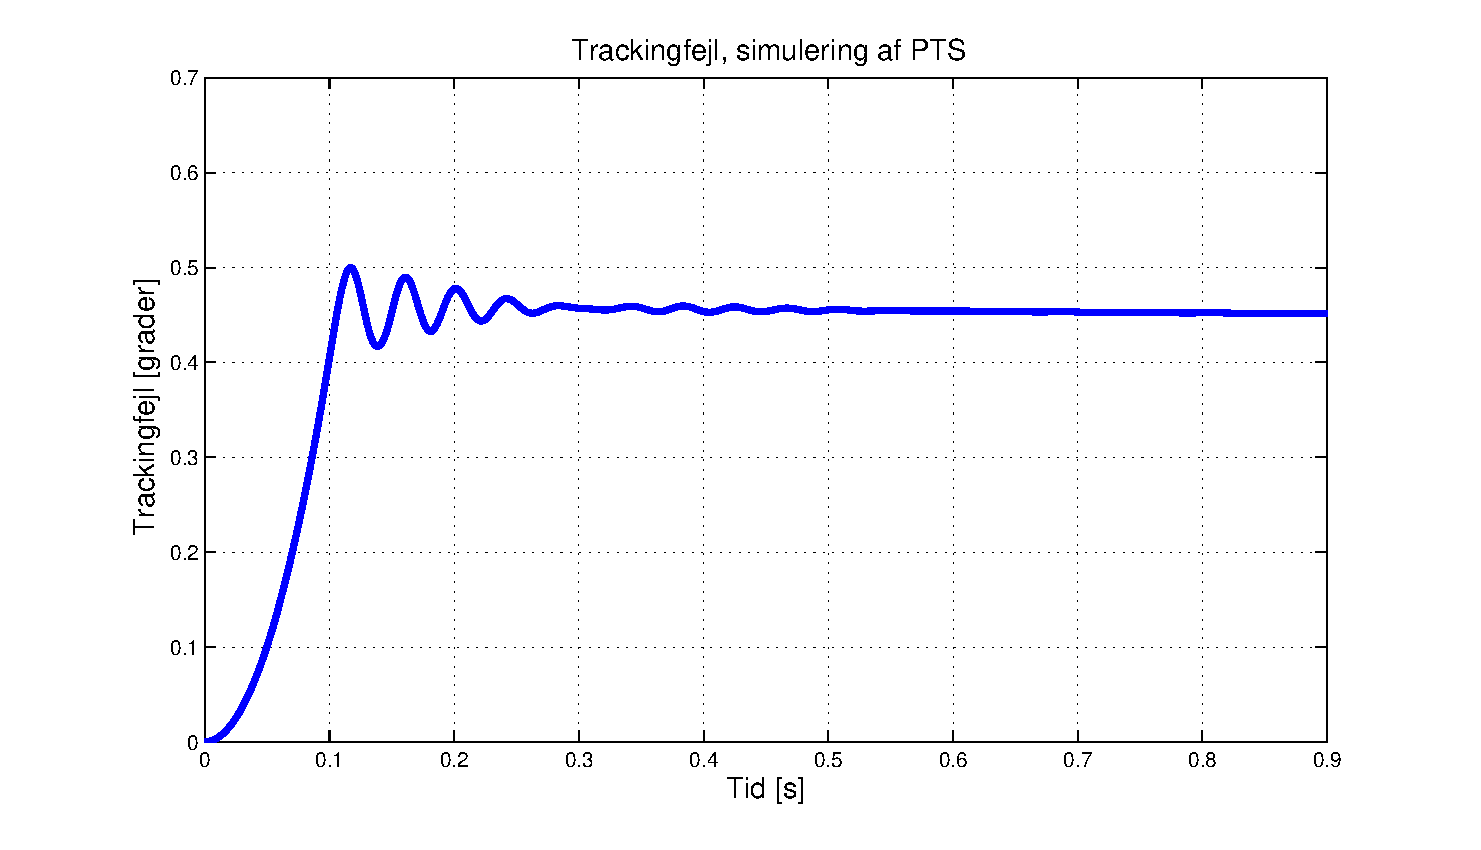
\includegraphics[width=0.7\textwidth]{./graphics/pidSim1.eps}
\captionsetup{width=0.6\textwidth}
\caption[Trackingfejl ved simulering]{Trackingfejl ved simulering af PTS med regulatorkoefficienterne fra tabel \ref{tb:pidSimulink}.} 
\label{fig:pidSim1}
\end{figure}
\todo[inline, color=red!20]{Denne test skal svare til en test vi laver på det rigtige system. Ellers er det ubrugeligt at se på en fejl og sammenligne den med en anden fejl i en anden situation}
De to regulatorer er med koefficienterne i tabel \ref{tb:pidSimulink} blevet afprøvet i praksis.
Figur \ref{fig:pidPhys1} viser pan og tilt-fejlsignalet i forhold til den kontinuerte lerdueparabel fra applikationen.

\begin{figure}[h!]
\centering
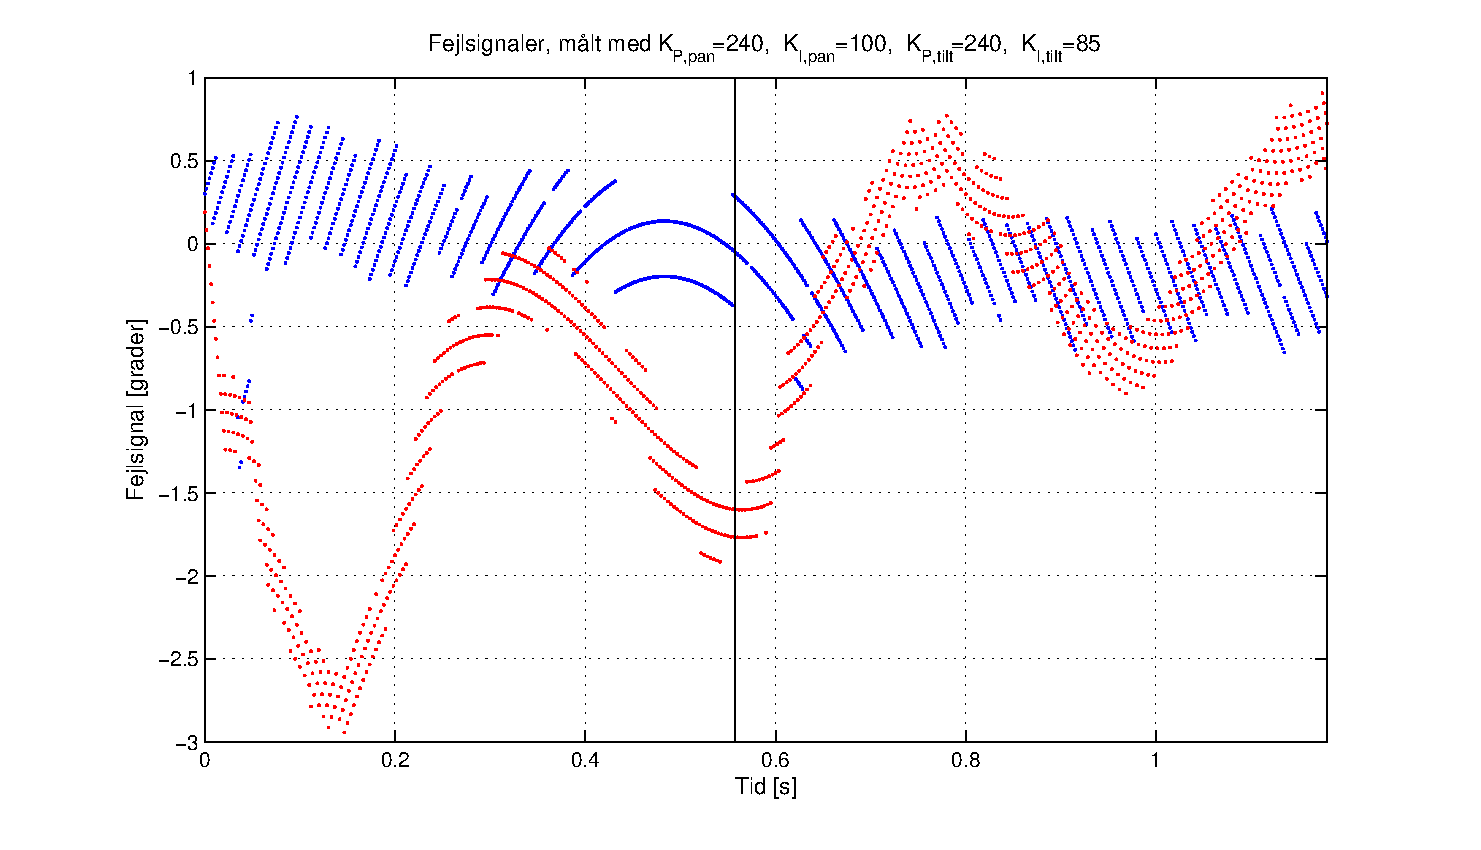
\includegraphics[width=0.7\textwidth]{./graphics/pidPhys1.eps}
\captionsetup{width=0.6\textwidth}
\caption[Fejlsignaler m. startkoefficienter]{Fejlsignaler m. startkoefficienterne fra tabel \ref{tb:pidSimulink}.
	De sorte lodrette streger angiver \(t_s=0,557 \text{ [s]}\).
	Pan-fejlsignalet er markeret med krydser, og tilt-fejlsignalet er markeret med prikker.} 
\label{fig:pidPhys1}
\end{figure}
\todo[inline, color=red!20]{En farve til tilt, en farve til pan. ingen kan se krydser eller prikker fra denne afstand.
Der er en enkel måling som ødelægger vores forsøg. Vi kan ikke vurdere at en tilt fejl på 0,9 er godt nok}


Som det ses på figur \ref{fig:pidPhys1} giver regulatoren til tilt et fejlsignal,
der maks. afviger 0,9\degree{} efter \(t_s\).
Pan-fejlen afviger derimod op til 1,8\degree{} efter \(t_s\).
Trackingfejlen er altså langt større end kravet på maksimalt 1,02\degree.
Det vurderes en yderligere manuel justering af koefficienterne på pan-regulatoren nødvendig.
Det vurderes på baggrund af det lave fejlsignal ved tilt at den fundne
PI-regulator for tilt er anvendelig i praksis.


\section{Manuel justering ift. fysisk PTS}
Ved at ændre på koefficienterne og analysere fejlgraferne justeres performance 
hen mod det ønskede.

På pan er der behov for en hurtigere og mere dæmpet reaktion,
og det vurderes derfor, at der på pan er brug for en PID-regulator.

\subsection{Valg af integratormætning}
Det vælges at sætte integratormætningen til 100 for begge regulatorer, da det vurderes, at der drages
fuld nytte af integratorleddet når \( K_I \cdot Integrator_{Max} > PWM_{Max} \).

\subsection{Tilføjelse af et D-filter}
Undervejs i den manuelle justering af PID-regulatoren til pan blev det fundet, at D-leddet ikke udnyttedes til fulde,
og at kravene ikke kunne overholdes med PID-regulatoren som den var.
Det valgtes derfor at tilføje et filter til D-leddet. 
Det betyder at D-leddet nu vægter tidligere ændringer i fejlsignalet. 
Filtret reducerer peaks i det differrentierede fejlsignal, der skyldes Zero Order Hold i upsamplingen (se afsnit \ref{subsec:upsampling}).

Der implementeres et 4. ordens FIR filter. Filtret er designet i MATLAB's grafiske fdatool og gør brug af at Kaiser vindue.
Filtrets step- og frekvensrespons kan ses på figur \ref{fig:d_filter_step} hhv. \ref{fig:d_filter_bode}. 

\begin{figure}[h!]
\centering
\subfloat[Steprespons for det implementerede filter.\label{fig:d_filter_step}]{%
	\hspace*{-0.6cm}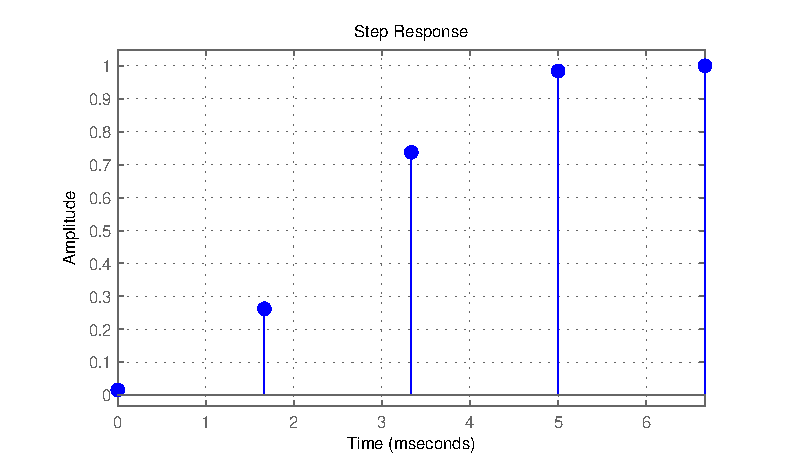
\includegraphics[width=0.57\textwidth]{./graphics/d-filter-step-small}
}
\subfloat[Frekvensrespons for det implementerede filter.\label{fig:d_filter_bode}]{%
	\hspace*{-1.15cm}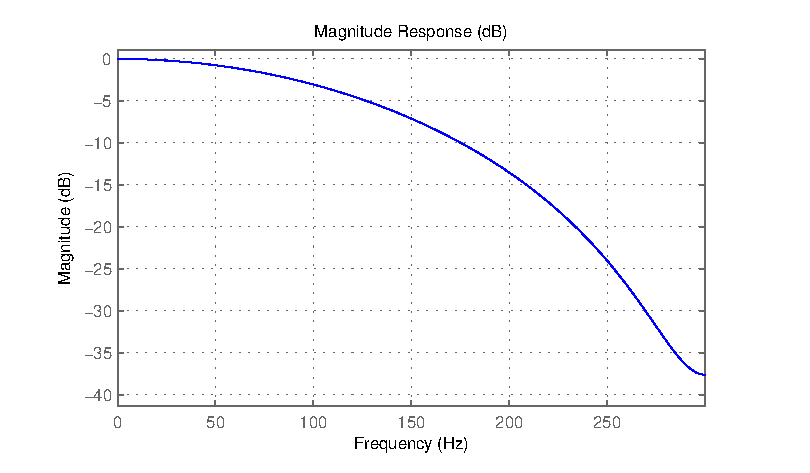
\includegraphics[width=0.57\textwidth]{./graphics/d-filter-bode-small}
	
}
\caption[D-filterets respons]{D-filterets step- og frekvensrepons.}
\label{fig:d_filter}
\end{figure}

\todo[inline, color=red!20]{større tidsakse så første og sidste spike kan ses}

\section{Endelig performance}
Efter adskillige test og finjustering af regulatoren, vurderes det at 
koefficienterne i tabel \ref{tb:PID_final} giver den bedst mulige performance 
for PTS. Denne performance ses i \ref{fig:PID_final}. Det ses at trackingfejlen 
holder sig inden for de 1,02$\degree$  pånær ved et par enkelte samples.

\begin{figure}[h!]
\centering
\begin{tabu}{l|[1.25pt]c|c|c}
      & \(K_P\) & \(K_I\) & \(K_D\)\\\tabucline[1.25pt]{-}
Tilt  & 240 & 85 & -\\\hline
Pan   & 100 & 110 & 3,8
\end{tabu}
\captionsetup{type=table}
\caption[Endelige regulatorkoefficienter]{De endelige regulatorkoefficienter.}
\label{tb:PID_final} 
\end{figure}

\begin{figure}[h!]
\centering
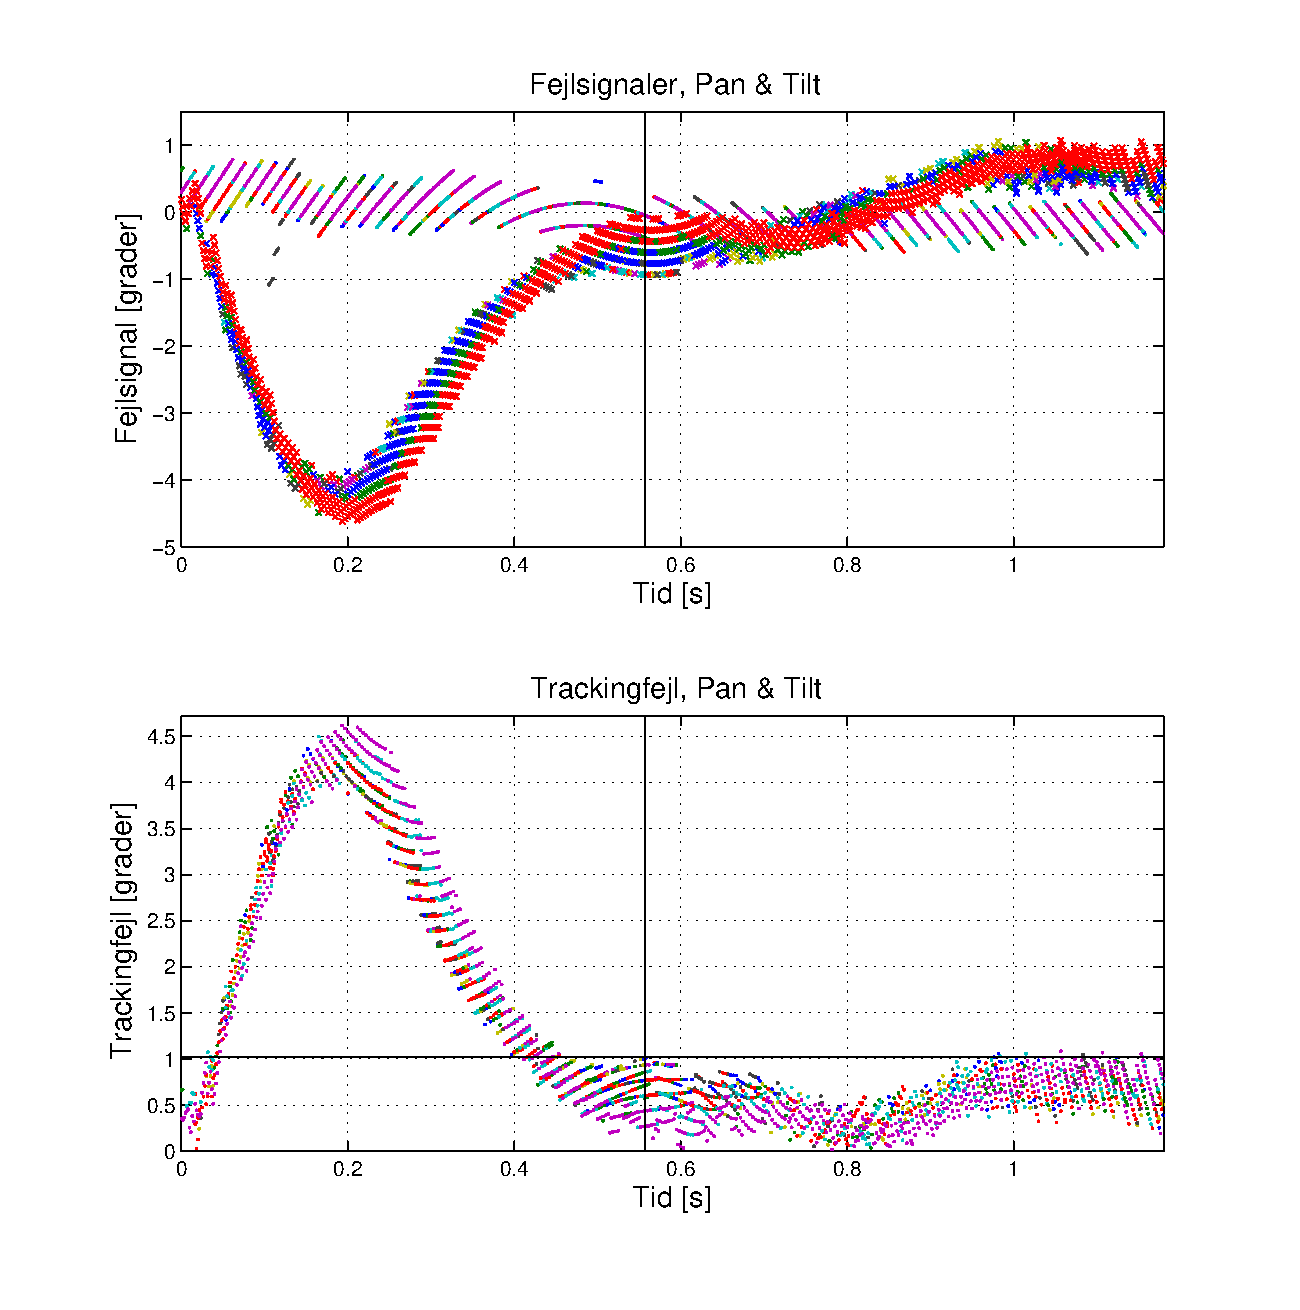
\includegraphics[width=1\textwidth]{./graphics/pidPhys2.eps}
\caption[Endelig performance]{Endelig performance. Fejlsignaler for Pan (krydser) og Tilt (prikker) øverst, trackingfejl nederst.
Testen er foretaget med koefficienterne fra tabel \ref{tb:PID_final}.
De sorte streger angiver kravene om Settling Time på under 0,557 [s] og trackingfejl på under 1,02\degree{}.} 
\label{fig:PID_final}
\end{figure}

\todo[inline, color=red!20]{vi skal kigge på hvor meget vi er uden for og beskrive dette}

%
%\begin{figure}[h!]
%\centering
%\begin{tabu}{l|[1.25pt]c|c|c}
%      & \(K_P\) & \(K_I\) & \(K_D\)\\\tabucline[1.25pt]{-}
%Tilt  & 49 & 32,5 & 0\\\hline
%Pan   & 80 & 160 & 3,55
%\end{tabu}
%\captionsetup{type=table}
%\caption[Endelige regulatorkoefficienter]{De endelige regulatorkoefficienter.}
%\label{tb:PID_final} 
%\end{figure}
%
%\begin{figure}[h!]
%\centering
%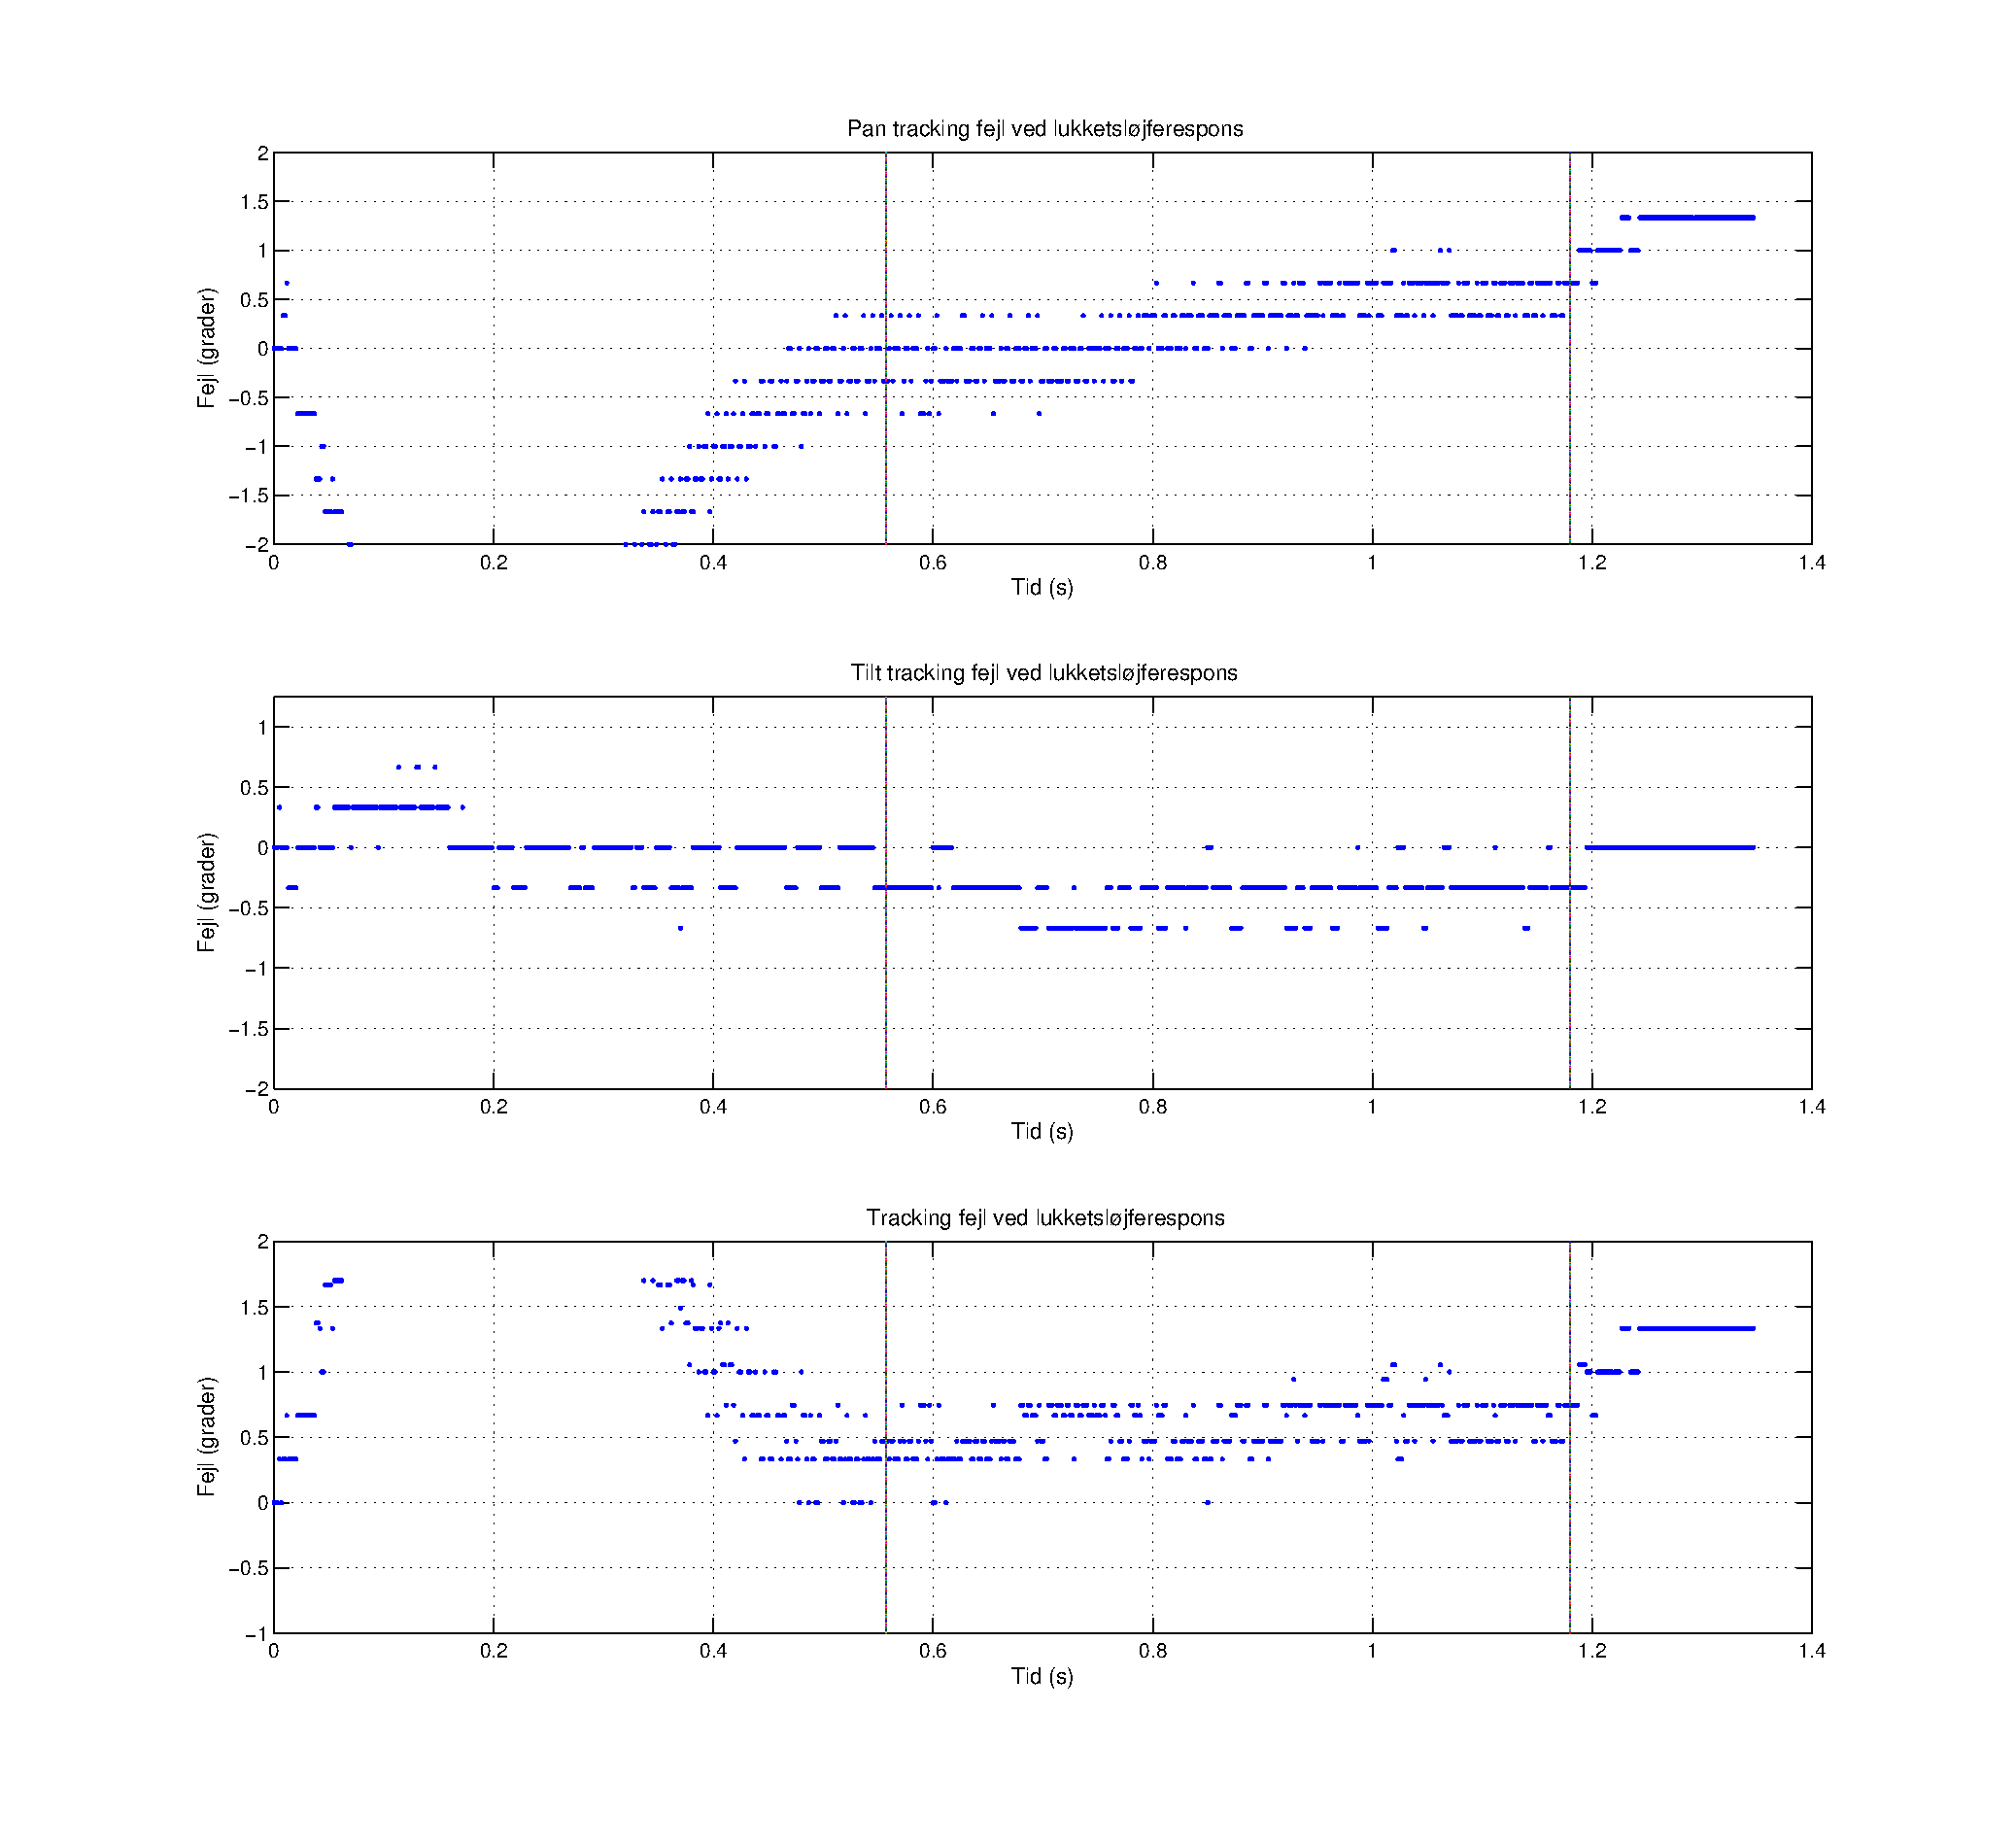
\includegraphics[width=1\textwidth]{./graphics/error_slut.eps}
%\caption[Endelig regulator koefficienter]{Trackingfejl målt i grader for hhv. pan og tilt samt den samlet trackingfejl. Testen tager udgangspunkt i koefficienterne fra  tabel \ref{tb:PID_final} og det ses at den samlet trackingfejl opfylder kravet til PTS.} 
%\label{fig:PID_final}
%\end{figure}

Det viste sig under justeringen at systemet er meget følsomt overfor slid i drivremmene mellem motorerne og Pan- og Tilt-rammerne.
Systemet kræver derfor kalibrering for at kunne fungere i praksis.

\section{Delkonlusion}
Ved Trial-\&-Error-metoden blev regulatorkoefficienterne i Simulink justeret til at give den ønskede 
tracking performance ift. et parabelinput. Pan-koefficienterne giver dårlig performance i praksis.
Ved manuel justering blev et sæt PID-regulatorkoefficienter fundet til Pan, som gav bedre performance.
Det vurderedes nødvendigt at implementere et lavpasfilter til D-leddet.
Med det implementerede filter gav de justerede regulatorkoefficienter en performance,
der ikke ved alle forsøg levede op til kravspecifikationen. Ved nogle af forsøgene viste
systemet sig at leve op til kravene om en trackingfejl på under 1,02\degree efter 0,557 [s].
Systemet er følsomt overfor slid i drivremmene.
%\section{PTS verifikation}

%\part{Test}
\todo[inline, color=pink,author=Mikkel]{Her bør være test der kan vise om vi kan opfylde kravene fra problemformuleringen.}
\part{Evaluering}
Denne del opsummerer projektarbejdet gennem diskussion og konklusion. 

\section{Diskussion}
\label{sec:diskussion}
Den matematiske model for PTS fundet på baggrund af
målinger af motorparametre og beregning af inertimomenter
er til en vis grad blevet verificeret vha. en test af åbensløjferesponsen.
Den største mangel ved den matematiske model er, at den ikke indeholder en dødzone
af PWM-duty cycles, der ikke kan accelerere systemet. Det vurderes
at simuleringen af systemet er nøjagtig, når der tages højde for dødzonen.

Reguleringssystemet er blevet simuleret i MATLAB Simulink, og på baggrund af denne simulering
er to sæt af regulatorparametre \(K_p\) og \(K_i\) til to PI-regulatorer blevet fundet.
Disse parametre vurderes til at skulle justeres
i forhold til eksperimentelle målinger på det fysiske system, da simuleringen kun er en tilnærmelse.

Regulatorernes parametre justeres vha. "trial and error"
med udgangspunkt i simuleringsresultaterne.
Justeringen viste, at det i praksis er nødvendigt at anvende en PID-regulator til Pan-systemet,
og at de vha. simuleringen fundne regulatorparametre \(K_p\) og \(K_i\) for Tilt fungerer godt i praksis.
%Desuden blev det under justeringen fundet, at det kan forbedre regulatorernes ydeevne
%at justere dødzone-værdierne for Pan- og Tilt-systemerne.


Reguleringssløjfernes realtidskrav er blevet opfyldt af implementeringen på mikrocontrolleren,
og det vurderes derfor at den anvendte software-struktur og valget af skedulering
er passende til trackingen af lerdueparablen.
FPGA'en genererer PWM-signalerne og leverer positionsfeedback med høj hastighed,
og SPI-kommunikationens afviklingstid varierer meget lidt fra gang til gang.
Det vurderes derfor, at den digitale controllers forsinkelser samlet set ikke forværrer
reguleringens ydeevne betydeligt.

De to regulatorer overholder ikke altid kravspecifikationen.
I nogle forsøg opfylde systemet dog kravene om en trackingfejl på under 1,02\degree{}
efter 0,557 [s].
Systemet tillader ikke megen parametervariation
som slid i drivremmene,
og det vurderes derfor, at mere avancerede regulatorer ville være mere velegnet til trackingen
af parablen.
\section{Konklusion}
\label{sec:konklusion}
Et Pan \& Tilt-system er blevet opbygget til nedskydning af en lerdue i English Skeet.
Med udgangspunkt i en matematisk model af systemet er to digitale regulatorer
blevet designet: En PID-regulator til pan-systemet og en PI-regulator til tilt-systemet.

Regulatorerne er implementeret på en mikrocontroller, og modtager positionsfeedback
fra en FPGA gennem SPI.
Reguleringssløjfernes realtidskrav imødekommes ved brug af operativsystemet FreeRTOS.

Efter manuel justering af PID-regulatoren til pan-systemet er det blevet fundet,
at kravene til systemets performance ikke kan imødekommes i alle tilfælde.
I nogle af de udførte tracking-forsøg var systemet dog i stand til at følge lerduens bevægelse
iht. kravspecifikationen,
og i alle forsøgene fulgtes bevægelsen nøjagtigt i min. 0,42 [s] efter lerduen havde nået sit toppunkt.

\section{Videreudvikling}
En højere opløsning på vinklen kunne have forbedret performance og givet mere nøjagtig tracking af lerduen.
Dette kan opnås ved flere Hall sensorer monteret på motorerne, eller ved en anden gearing på PTS.
Hvis fx gearingen ændredes fra 1:3 til 1:6 ville opløsningen blive fordoblet. Samtidig ville responsens tophastighed
blive sænket. Videre arbejde kunne altså undersøge mulighederne for mere nøjagtig tracking af lerduen og deres
indflydelse på performance i tidsdomænet.

Til hurtigere respons på trackingen ville en mere avanceret regulator muligvis kunne anvendes.
Fx. kunne videre arbejde omfatte design af en regulator til det koblede system.
Samtidig ville det være af høj relevans at minimere følsomheden overfor slid i drivremmene,
enten ved at erstatte drivremmene med mere slidstærke varianter, eller ved løbende tilpasning
af regulatoren til parametervariationen i PTS's overføringsfunktioner.
En undersøgelse af andre filtreringsmuligheder for D-leddets filter i PID-regulatoren ville kunne kaste
lys over, om det implementerede D-filter er optimalt til applikationen.
Reguleringen ville kunne forbedres ved forudsigelse af lerduens bevægelse med interpolation
af de samplede koordinater for lerduen.
Videre arbejde med systemet til samme applikation burde udnytte,
at lerduens bevægelse tilnærmelsesvis er parabelformet og dermed forudsigelig.
%%%%%%%%%%%% Litteratur %%%%%%%%%%%%
\bibliography{litteraturliste}
%%%%%%%%%%%% Appendix %%%%%%%%%%%%
\part{Appendices}
\appendix
\addtocontents{toc}{\protect\setcounter{tocdepth}{1}} % Antal niveau af appendix i indholdsfortegnelsen.
\section{Lerduens karakteristika}
\label{sec:udregning_af_parabel}

Jævnfør reglerne for ES, skal lerduen passere target crossing point (TCS) som er 
placeret i 4,57 [m] over origo med en fejlmargin på \(\pm\)0,45 [m] for passagen. 
Lerduen skal flyve 50 [m] - 52 [m]. "High House" er placeret 20,11 [m] fra TCS, i en 
højde af 3,05 [m]. 

\subsection{Parabel i 2 dimensioner}
For at simplificere udregningerne, bestemmes parablen først i 2D. Når denne er fundet kan den tredje dimension tilføjes.\\

Da luftmodstanden er negligerbar kan parablen (2. grads polynomium) findes ved at indsætte de kendte punkter. Kasteparablen er givet ved vektorfunktionen i ligning \ref{eq:pf:vektorparabel}.

\begin{equation}
	Pos(t) = \left( \begin{array}{c}
	x_{2D}(t) \\
	y_{2D}(t)
	\end{array}
	\right)
	= \left( \begin{array}{c}
	\cos \theta v_0 t + x_0 \\
	\sin \theta v_0 t - \frac{g}{2} t^2 + y_0
	\end{array}
	\right)
\label{eq:pf:vektorparabel}
\end{equation}

Hvor \(\theta\) er afskydningsvinklen, \(v_0\) er afskydningshastigheden, \(g=9,82 \left[ \frac { m }{ { s }^{ 2 } } \right] \) er tyngdeacceleration og \(x_0\), \(y_0\) er begyndelsespunktet. 

For at få en parabel på formen y(x), isoleres t i x(t) med henblik på at substituere t i y(x): (\(x_0\) sættes til 0.)

\begin{equation}
t = \frac{x}{\cos \left( \theta \right) v_0}
\label{eq:pf:x(t)}
\end{equation}

Den fundne værdi for t indsættes i \(y(t)\) og udtrykket reduceres, \citep[Side. 67]{fund_of_physics}.
\begin{align}
\begin{split}
y(t(x)) &= \sin \left( \theta \right) \frac{x}{\cos \left( \theta \right) v_0} v_0 - \frac{g}{2} \left(\frac{x}{\cos \left( \theta \right) v_0}\right)^2 + y_0 \\
y(x) &= \tan \left( \theta \right) x - \frac{gx^2}{2(\cos \left( \theta \right) v_0)^2} + y_0
\label{eq:pf:y(x(t))}
\end{split}
\end{align}

Det ses at der er 3 ubekendte i ligningen. I reglerne for ES affyres lerduerne fra en højde af \(y_0\) = 3,05 [m].
\begin{equation}
y(x) = \tan \theta x - \frac{gx^2}{2(\cos \left( \theta \right)  v_0)^2} + 3,05
\label{eq:pf:y(x)2}
\end{equation}
I reglerne fremgår det at lerduens flugt passere TCS, som er placeret i en højde på 4,57 [m], 20,11 [m] fra HH. Det sidste krav er at lerduen først skal ramme jorden efter 50 [m] - 52 [m], (52 [m] i projektet). \\
Det giver koordinatsættene (20,11 ; 4,57) og (52 ; 0). Vha. disse bestemmelser er udtrykkes \(\theta\) og \(v_0\).

\begin{eqnarray}
\theta &=& 9,103 \degree \\
v_0 &=& 34,589 \left[ \frac { m }{ s }  \right] 
\end{eqnarray}

 \(\theta\) og \(v_0\) indsættes i stedvektoren fra ligning \ref{eq:pf:vektorparabel} samt udtrykket fra ligning \ref{eq:pf:y(x)2}, hvorefter de reduceres.

\begin{align}
\begin{split}
	Pos(t) = \left( \begin{array}{c}
	x_{2D}(t) \\
	y_{2D}(t)
	\end{array}
	\right)
	&= \left( \begin{array}{c}
	\cos \left(9,103 \degree \right) 34,589 t \\
	\sin \left(9,103 \degree \right) 34,589 t - \frac{9,82}{2} t^2 + 3,05
	\end{array}
	\right) \\
% ------------------------------
	&= \left( \begin{array}{c}
	34,153 t \\
	- 4,91 t^2 + 5,473 t + 3,05
	\end{array}
	\right)
\label{eq:pf:vektorparabel2}
\end{split}
\end{align}
\begin{align}
\begin{split}
y(x) &= \tan \left(9,103 \degree \right) x - \frac{9,82x^2}{2(\cos \left(9,103 \degree \right) 34,589)^2} + 3,05 \\
% -------------------------------
&= - 0,00421 x^2 + 0,1602 x  + 3,05
\label{eq:pf:y(x)3}
\end{split}
\end{align}
Ovenstående ligning \ref{eq:pf:y(x)3} og ligning \ref{eq:pf:vektorparabel3d} bruges til bestemmelse af tiden, hvor lerduen når SB-afstanden.

\subsection{Parabel i 3 dimensioner}
\label{subsubsec:para}
Nu omskrives parablen fundet i ligning \ref{eq:pf:vektorparabel2} til x,y,z koordinater. 
Grundplanet er xy og højden er givet ved z. Dvs. at \(z(t) = y_{2D}(t)\) og at \(x(t)\) samt \(y(t)\) afhænger af \(x_{2D}(t)\) samt vinklen \(\alpha\). 
\(\alpha\) er givet ved vinklen mellem parablen projekteret ned på xy-planet (som vist på figur \ref{fig:para_in_xy_plane}) og y-planet.
%\todo[inline, author=Michael, color=blue! 50]{Kan også skrives som vinklen mellem parablen og x,z planet?}
Stedvektoren for lerduens position i 3D er givet i nedenstående ligning, hvor \(\alpha = 15,872 \degree\).
\begin{align}
\begin{split}
Pos\left( t \right) = 
\left( \begin{matrix} x\left( t \right)  \\
 y\left( t \right)  \\ 
 z\left( t \right)  \end{matrix} \right) &=
 \left( \begin{matrix} - sin\left( \alpha  \right) \cdot { x }_{ 2D }\left( t \right) + 5.5 \\
 cos\left( \alpha  \right) \cdot { x }_{ 2D }\left( t \right) - 19.3  \\
  { y }_{ 2D }\left( t \right)  \end{matrix} \right)
\\
%----------------------------------------
&= \left( \begin{matrix} - 9,34\cdot t+5,5 \\
  32,851\cdot t-19,3 \\ 
 -{ 4,91\cdot t }^{ 2 }+5,473\cdot t+3,05\end{matrix} \right) 
\label{eq:pf:vektorparabel3d}
\end{split}
\end{align}




Bemærk udgangspunktet for kastet er flyttet fra origo, til HHs position. (Punkt D på figur \ref{fig:para_in_xy_plane}).

\section{DC motoren}
Dette appendix beskæftiger sig med bestemmelsen af motorparametrene.
\subsection{DC Motor karakteristik}
DC Motoren kan modelleres efter diagrammet på fig. \todo[inline]{kredsløbsdiagram skal indsættes}\todo[inline]{Kildehenvisning til DC motor model}.
Ligningen for \(V_m\) er givet ved ligning \ref{eq:Vm_transient0}.
\begin{equation}
	V_m(t)=L_m \cdot \frac{\mathrm d}{\mathrm d t} \big( i_m(t) \big)+R_m \cdot i_m(t) + V_{EMF}(t)
	\label{eq:Vm_transient0} 
 \end{equation}
Den modelektromotoriske kraft, \(V_{EMF}\) er givet ved ligning \ref{eq:VEMF}.
\begin{equation}
	V_{EMF}(t) = K_b \cdot \omega(t)
	\label{eq:VEMF}
\end{equation}
Med ligning \ref{eq:VEMF} kan ligning \ref{eq:Vm_transient0} omskrives til ligning \ref{eq:Vm_transient1}.
\begin{equation}
	V_m(t)=L_m \cdot \frac{\mathrm d}{\mathrm d t} \big( i_m(t) \big)+R_m \cdot i_m(t) +K_b \cdot \omega(t)
	\label{eq:Vm_transient1} 
 \end{equation}

Kraftmomentet kan udtrykkes som funktion af strømmen, som i ligning \ref{eq:Tm_im}.
\begin{equation}
	T_m(t)=K_t\cdot{i_m(t)}
	\label{eq:Tm_im} 
 \end{equation}
Samtidig kan kraftmomentet, som motoren producerer, udtrykkes som multiplikationen af inertimoment og vinkelacceleration.
Det inertimoment, der leveres til belastningen vil være kraftmomentet fra motoren fratrukket friktionen.
Friktionen antages til disse beregninger at være viskøs, dvs. proportional med vinkelhastigheden.
Kraftmomentet kan altså udtrykkes ved ligning \ref{eq:Tm_leveret}
\begin{equation}
	T_m(t)=J\cdot\frac{\mathrm d}{\mathrm d t} \big(\omega(t) \big)+B\cdot\omega(t)
	\label{eq:Tm_leveret} 
 \end{equation}

Proportionalitetskonstanterne \(K_b\) og \(K_t\) har i SI-enheder samme numeriske værdi\todo{KILDE!}.

\subsection{Eksperiment 1}
\label{ss:eksperiment1}
\subsubsection{Formål}
Bestemmelse af motorens ækvivalente resistans, \(R_m\).
\subsubsection{Teori}
Forhindres motoren i at rotere, vil vinkelhastigheden være nul.
Hvis man påfører motoren en DC-spænding \(V_m\),
og venter til motorens respons har nået steady-state,
så vil strømmen igennem motoren være konstant.
Her vil ligning \ref{eq:Vm_transient1} kunne omskrives til ligning \ref{eq:resistans_E1}.
\begin{equation}
	V_m=R_m \cdot i_m
	\label{eq:resistans_E1} 
 \end{equation}
Målinger af sammenhørende steady-state værdier for strøm \(i_m\) og spænding \(V_m\)
kan altså bruges til bestemmelse af den ækvivalente resistans \(R_m\).
\subsubsection{Fremgangsmåde}
Motoren låses fast vha. en skiftenøgle og påføres en lav spænding.
Efter nogle sekunder, når transientresponsen er væk,
måles spændingen over og strømmen igennem motoren med multimetre.
Værdierne noteres, og forsøget gentages ved andre spændinger.

De anvendte multimetre er af typen TTi 1604.
\subsubsection{Måleresultater}
I tabel \ref{tb:resistans} findes målingerne af strøm og spænding.\todo[inline,color=blue! 50]{Mikael, jeg synes de vil se bedre ud i tabellen, hvis der 
var et mindre decimal i de ni første, \(V_m\).}
\begin{figure}[th!]
	\centering
	%\begin{tabular}{r|r}
%$V_m$ [V]&$i_m$ [A]\\\hline
%0,509&0,094 \\ %0,5093&0,094 \\
%0,883&0,172 \\ %0,8833&0,172
%1,481&0,297 \\ %1,4809&0,297 
%1,940&0,391 \\ %1,9404&0,391
%2,345&0,470 \\ %2,3448&0,470
%2,788&0,555 \\ %2,7879&0,555
%3,182&0,638 \\ %3,1823&0,638
%3,465&0,664 \\ %3,4652&0,664
%3,835&0,746 \\ %3,8346&0,746
%4,067&0,765 \\ % 4,067&0,765
%4,292&0,830 \\ %4,292&0,830 
%\end{tabular}


\begin{tabular}{r|r|r|r|r|r|r|r|r|r|r|r}
$V_m$ [V]&0,509&0,883&1,1481&1,940&2,345&2,788&3,182&3,465&3,835& 4,067&4,292\\\hline
$i_m$ [A]&0,094&0,172&0,297 &0,391&0,470&0,555&0,638&0,664&0,746&0,765&0,830
\end{tabular}
	\captionsetup{type=table}
	\caption[Sammenhørende værdier af DC spænding og strøm]
			{Sammenhørende værdier af DC spænding over og strøm gennem rotationslåst motor.}
	\label{tb:resistans}
\end{figure}
\subsubsection{Databehandling}
Den målte strøm-spændingskarakteristik for DC-motoren er indtegnet på figur \ref{fig:resistans0}.
\begin{figure}[th!]
	\centering
	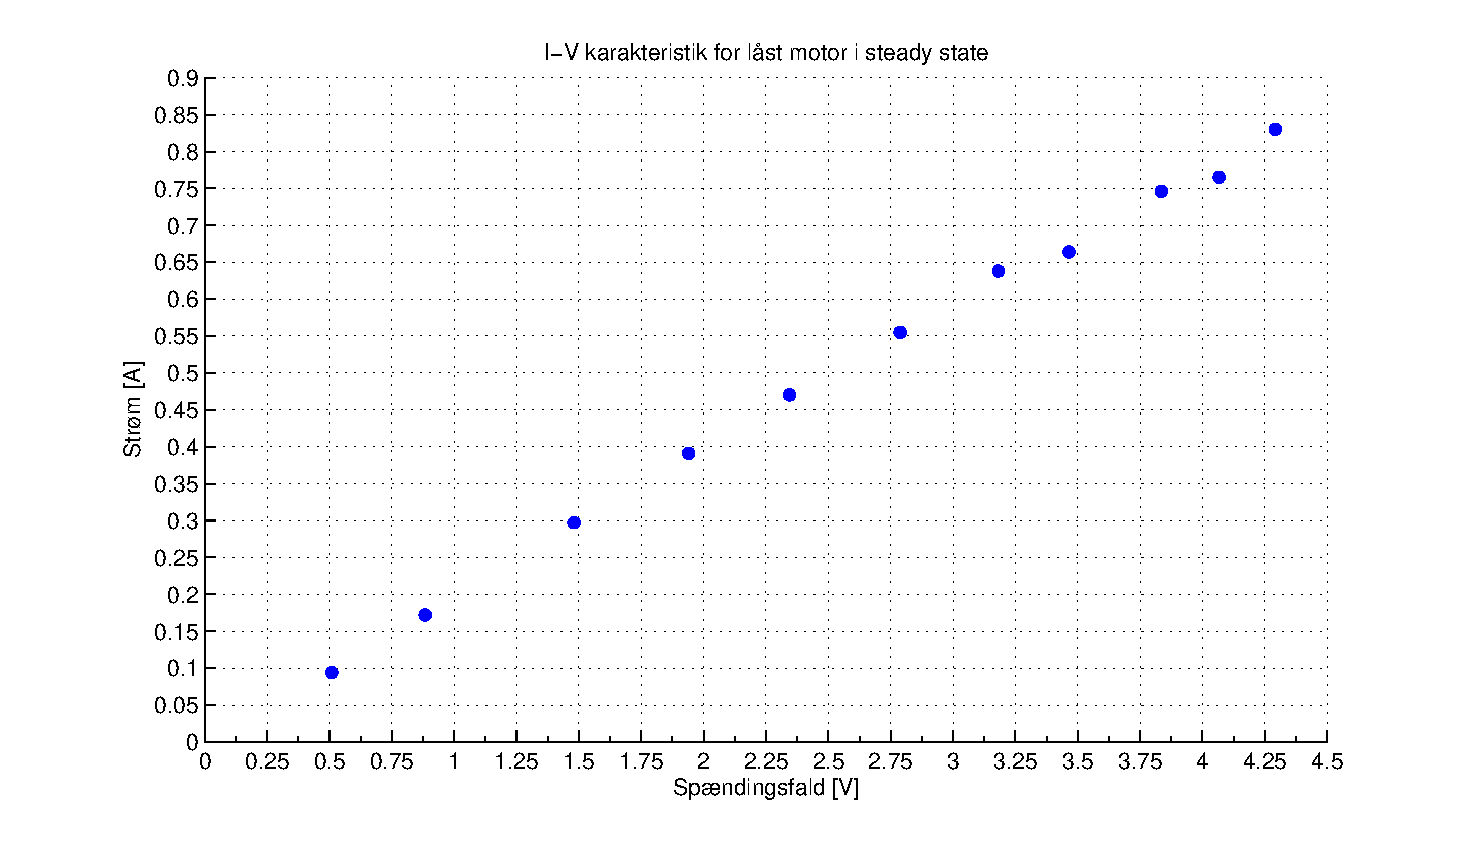
\includegraphics[width=1\textwidth]{./graphics/resistans1.eps}
	\caption[Strøm-spændingskarakteristik for rotationslåst DC-motor]{Strøm-spændingskarakteristik for rotationslåst DC-motor ved steady-state.}
	\label{fig:resistans0}
\end{figure}
Som det ses på figur \ref{fig:resistans0} er sammenhængen mellem strøm og spænding
tilnærmelsesvis lineær, og en lineær regression på dataene vil altså give en tilnærmet værdi for \(R_m\).
\(R_m\) er ved lineær regression beregnet til 5,21 \([\Omega]\). \todo{Flere decimaler?}

Den i forsøget mindste afsatte effekt i motoren er 48 [mW].
\subsubsection{Diskussion}
Da sammenhængen mellem strøm og spænding i målingerne er tilnærmelsesvis lineær,
vurderes den fundne værdi for \(R_m\) at være meget nøjagtig,
om ikke andet, så for effektafsættelser i motoren på mindst 48 [mW].
\subsubsection{Konklusion}
Motorens ækvivalente resistans, \(R_m\) er vha. sammenhørende målinger af strøm og spænding
for en rotationslåst motor, ved effektafsættelser i motoren på 48 [mW] og højere,
blevet bestemt til 5,21 \([\Omega]\). \todo{Flere decimaler?}
\subsection{Eksperiment 2}
\label{ss:eksperiment2}
\subsubsection{Formål}
Bestemmelse af motorens ækvivalente induktans, \(L_m\).
Der er benyttet to forskellige metoder til bestemmelsen af induktansen.
Metode 1 tager udgangspunkt i tidskonstanten for et RL-kredsløb,
mens metode 2 tager udgangspunkt i faseforskellen mellem forskellige komplekse impedanser i serie.
\subsubsection{Teori}
\paragraph{Metode 1}
Forhindres motoren i at rotere, vil vinkelhastigheden som beskrevet i afsnit \ref{ss:eksperiment1} være nul.
Ved denne metode er vi interesseret i systemets transientrespons, hvor strømmen \(i_m\) ikke er konstant.
Forbindes en modstand \(R_s\) i serie med DC-motoren som vist på fig. %\ref{fig:e2_rl1}
\todo[inline]{Indsæt kredsløbsdiagram med Rs}
vil der være tale om et RL-kredsløb, med en tidskonstant \(\tau\) givet ved ligning \ref{eq:rltimeconstant}.
Transientresponsen for alle strømme og spændingsfald i kredsløbet har denne tidskonstant.
\todo[inline]{Indsæt kilde eller forklaring til RL-tidskonstant.}
\begin{equation}
	\tau=\frac{L_m}{R_m+R_s}
	\label{eq:rltimeconstant} 
 \end{equation}
Tidskonstanten er et mål for tiden det tager systemet at opnå ca. 63,2 \% af slutværdien.\todo{D\&B-kilde}
For en (eksponentielt) aftagende kurve med tidskonstanten \(\tau\) kan tidskonstanten aflæses som
tidsforskellen mellem to niveauer V0 og V1, hvor V1 er ca. 36,8 \% af V0.

Ved omskrivning af ligning \ref{eq:rltimeconstant} kan induktansen altså bestemmes vha. ligning \ref{eq:induktans0}.
\begin{equation}
	L_m=\tau\cdot(R_m+R_s)
	\label{eq:induktans0} 
 \end{equation}
\paragraph{Metode 2}
Forhindres motoren i at rotere, vil vinkelhastigheden som beskrevet i afsnit \ref{ss:eksperiment1} være nul.
Ved denne metode er vi interesseret i systemets steady-state respons.
Forbindes en modstand \(R_{s1}\) i serie med DC-motoren som vist på fig. %ref{fig:e2_rl2}
\todo[inline]{Indsæt kredsløbsdiagram med Rs1 og AC-forsyning med DC offset}
vil impedansen \(\mathbf{Z_m}\) af DC-motoren være givet ved ligning \ref{eq:zm_0}.
\begin{equation}
	\mathbf{Z_m}=R_{s1}\cdot\frac{\mathbf{V_1}-\mathbf{V_2}}{\mathbf{V_2}}
			=R_{s1}\cdot\left(\frac{\mathbf{V_1}}{\mathbf{V_2}}-1\right)
			=R_{s1}\cdot\left(\frac{A_1}{A_2}\cdot{e}^{\phi}-1\right)
	\label{eq:zm_0} 
 \end{equation}
Bemærk at spændingsfaldene noteres med fed skrift for at indikere at her er tale om phasors (komplekse tal),
at \(A_1\) og \(A_2\) angiver amplituderne af \(\mathbf{V_1}\) og \(\mathbf{V_2}\),
samt at \(\phi=\phi_1-\phi_2\) angiver faseforskellen mellem de to signaler.
Denne faseforskel kan også udtrykkes ved tidsforsinkelsen \(\Delta{t}\) ganget med vinkelfrekvensen \(\omega\).
Ligning \ref{eq:zm_1} angiver impedansen på rektangulær form.
\begin{equation}
	\mathbf{Z_m}=R_{s1}\cdot\left(\frac{A_1}{A_2}\cdot{\cos (\phi)}-1\right)	%Realdel
	+\mathbf{j}\cdot{R_{s1}}\cdot\frac{A_1}{A_2}\cdot\sin(\phi)	%Imaginærdel
	\label{eq:zm_1} 
 \end{equation}
Samtidig vides det, at den rotationslåse motors impedans består af resistansen \(R_m\) samt
reaktansen \(X_m\), hvor \(X_m\) er reaktansen for en spole, altså \(\omega\cdot{L_m}\).
Motorens impedans kan altså også beskrives ved ligning \ref{eq:zm_2}, hvor \(\mathbf{j}\) er den imaginære enhed.
\begin{equation}
	\mathbf{Z_m}=R_m+\mathbf{j}\cdot\omega\cdot{L_m}
	\label{eq:zm_2} 
 \end{equation}
Sættes ligningerne \ref{eq:zm_1} og \ref{eq:zm_2} lig med hinanden
kan man altså udtrykke resistansen \(R_m\) og induktansen \(L_m\) som funktioner
af faseforskellen på \(\mathbf{V_1}\) og \(\mathbf{V_2}\),
hvilket giver ligningerne \ref{eq:Rm_0} og \ref{eq:Lm_0}.
\begin{equation}
	\mathbf{R_m}=R_{s1}\cdot\left(\frac{A_1}{A_2}\cdot{\cos (\phi)}-1\right)
	\label{eq:Rm_0} 
 \end{equation}
\begin{equation}
	\mathbf{L_m}=R_{s1}\cdot\frac{A_1}{A_2}\cdot\sin(\phi)
	\label{eq:Lm_0} 
 \end{equation}

Effektafsættelsen \(P_{avg}\) i en modstand R, påført en vekselspænding med amplituden V, givet ved ligning \ref{eq:effekt}.
\todo[inline]{Kildehenvisning til effektformel}
\begin{equation}
	P_{avg}=\frac{\left(V_{rms}\right)^2}{R}=\frac{\left(\frac{V}{\sqrt{2}}\right)^2}{R}
	\label{eq:effekt}
 \end{equation}
\subsubsection{Fremgangsmåde}
\paragraph{Metode 1}
En modstand \(R_s\) måles efter med et multimeter og fobindes i serie med DC-motoren
som på figur %\ref{fig:e2_rl1}
.
Kredsløbet bestående af DC-motoren og \(R_s\) påføres en kendt spænding.
Strømmen gennem kredsløbet afbrydes på strømforsyningen og spændingsfaldet
over \(R_s\) måles med et oscilloskop.
Dataene eksporteres og tidskonstanten bestemmes herudfra.

Det anvendte multimeter er af typen TTi 1604,
og oscilloskopet er af typen \todo{Oscilloskop?}.

\paragraph{Metode 2}
En modstand \(R_{s1}\) måles efter med et multimeter og forbindes i serie med DC-motoren
som på figur %\ref{fig:e2_rl2}
.
Kredsløbet påføres en kendt AC-spænding fra en funktionsgenerator med et DC-offset så spændingen
altid er positiv.
Da funktionsgeneratoren ikke skal overbelastes, skal \(R_{s1}\) vælges tilpas stor.
AC-spændingens frekvens er 10 [kHz].
Med et oscilloskop måles spændingsfaldene \(\mathbf{V_1}\) og \(\mathbf{V_2}\).
Dataene eksporteres og faseforskellen samt forholdet mellem amplituderne \(A_1\) og \(A_2\) bestemmes herudfra.
\subsubsection{Måleresultater}
\paragraph{Metode 1}
Seriemodstanden \(R_s\) er blevet målt til 61,77 \([Omega]\).
På figur \ref{fig:induktans0} er transientresponsen for spændingsfaldet over \(R_s\) indtegnet
sammen med de to spændingsniveauer, hvorudfra tidskonstanten bestemmes.
\begin{figure}[th!]
	\centering
	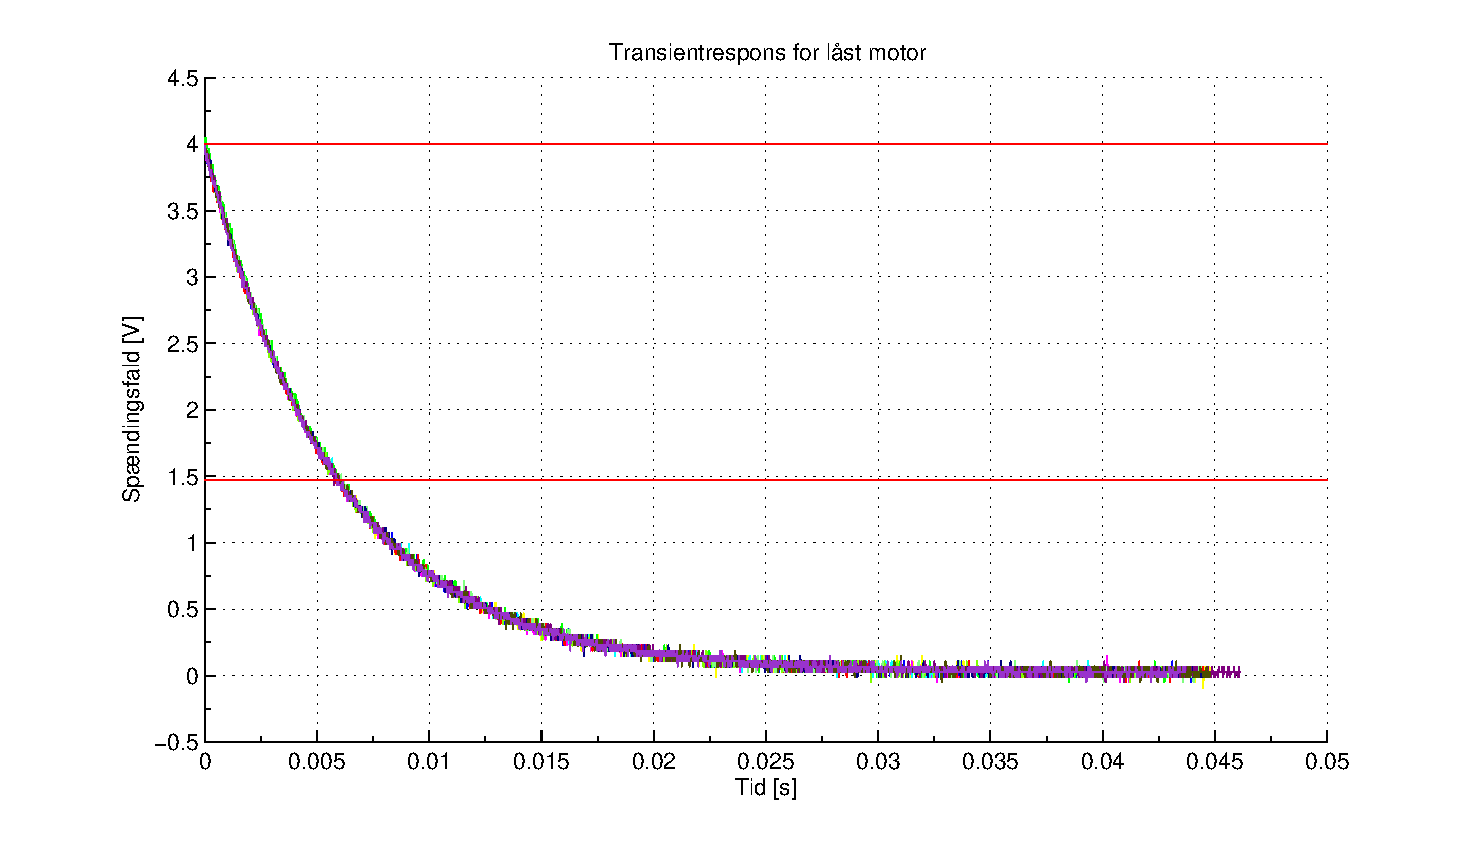
\includegraphics[width=1\textwidth]{./graphics/induktans0.eps}
	\caption[Transientrespons for låst motor]
		{Transientrespons for låst motor. De to vandrette røde linjer angiver spændingsniveauerne til bestemmelse af tidskonstanten.
		Den øverste linje er ved 4 [V], mens den nederste linje er ved 4 [V] \(\cdot \frac{1}{e}\).}
	\label{fig:induktans0}
\end{figure}
Figur \ref{fig:induktans0} viser flere målingers transientrespons.
\paragraph{Metode 2}
Seriemodstanden \(R_s1\) er blevet målt til 473,3 \([\Omega]\).
Spændingen har en amplitude på 2,4 [V] og et DC-offset på 2,5 [V].
På figur \ref{fig:induktans1} er steady-state responsen for spændingsfaldene over DC-motoren og seriemodstanden indtegnet.
\begin{figure}[th!]
	\centering
	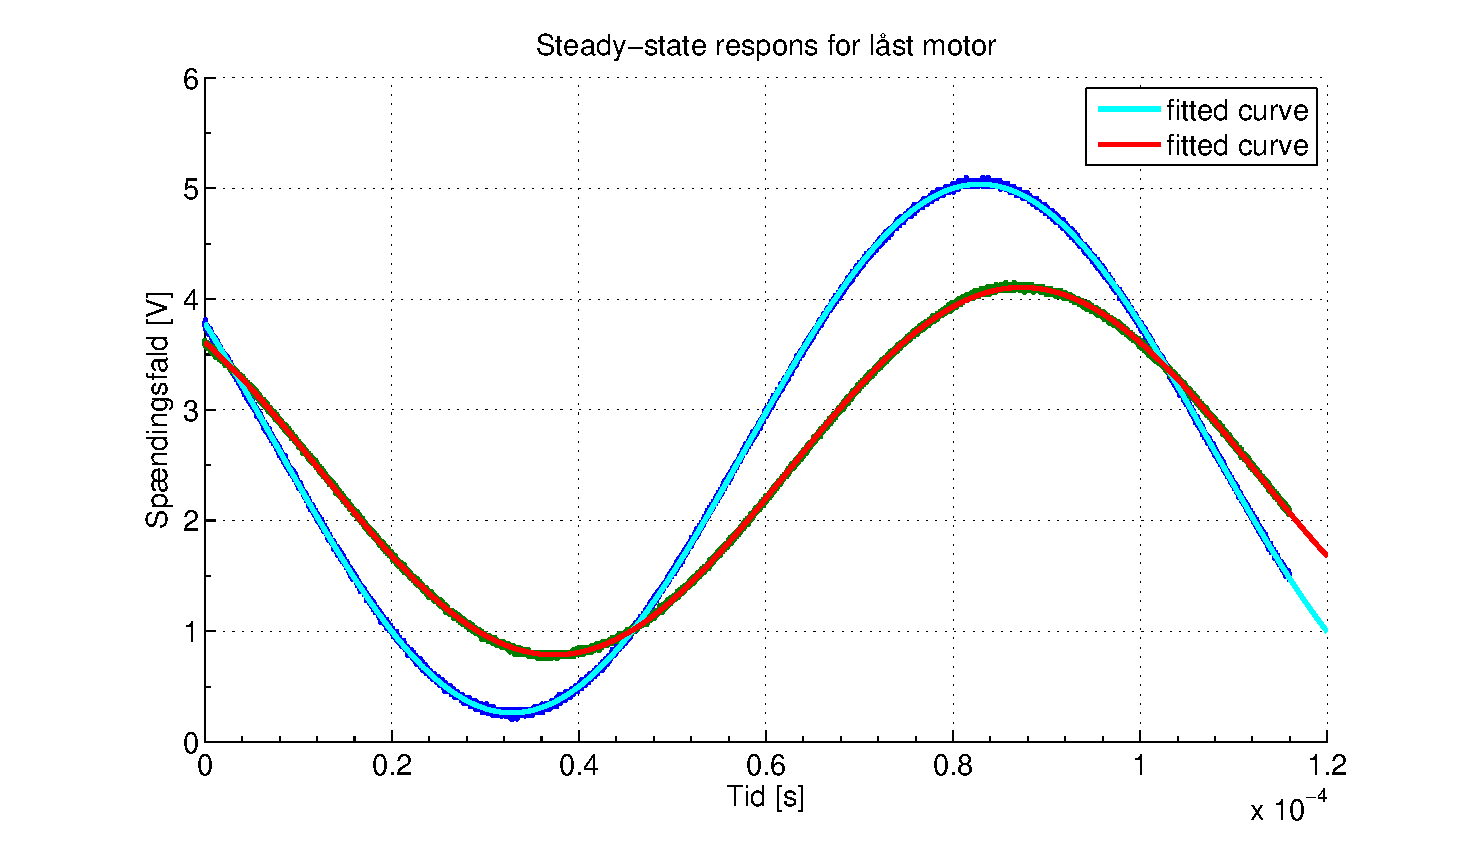
\includegraphics[width=1\textwidth]{./graphics/induktans1.eps}
	\caption[Steady-state respons for låst motor]
		{Steady-state respons for låst motor. Med mørkeblåt er markeret \(\mathbf{V_1}\) og med mørkegrønt \(\mathbf{V_2}\).
		To tilpassede sinuskurver, fundet vha. MATLAB's fit-funktion, er indtegnet med lyseblåt og rødt.}
	\label{fig:induktans1}
\end{figure}
\subsubsection{Databehandling}
\paragraph{Metode 1}
For hver måling af transientresponsen, vist i figur \ref{fig:induktans0} er induktansen blevet
bestemt ved brug af ligning \ref{eq:induktans0}.
Gennemsnitsinduktansen er ved denne metode blevet fundet til \(L_m=0,395\) [H].
\paragraph{Metode 2}
Vha. MATLAB's fit-funktion er to sinuskurver blevet tilpasset til de målte spændingsfald.
Ud fra funktionsforskrifterne på de to sinuskurver er amplitudeforholdet \(\frac{A_1}{A_2}\)
og faseforskellen \(\phi\) blevet beregnet,
og vha. ligningerne \ref{eq:Rm_0} og \ref{eq:Lm_0} er resistansen hhv. induktansen blevet beregnet til
179,94 \([\Omega]\) hhv. 3,047 [mH].
Effektafsættelsen i motoren er med amplitudeforskellen på \(\mathbf{V_1}\) og \(\mathbf{V_2}\) samt
de i forsøget fundne værdier \(R_{s1}\) og \(R_m\) ved brug af ligning \ref{eq:effekt} beregnet til 0,405 [mW].
\subsubsection{Diskussion}
Den lineære sammenhæng mellem strøm og spænding fundet i afnit \ref{ss:eksperiment1} kan ikke benægtes,
og for effektafsættelser i motoren på over 48 [mW] må resistansen kunne antages at være 5,21 \([\Omega]\) som beregnet.
Men, som fundet ved forsøget med metode 2, så er motorens resistans langt højere,
179,94 \([\Omega]\) ved en effektafsættelse i motoren på 0,405 [mW].
Dette indikerer, at motorens ækvivalente resistans er lineær i de brugbare intervaller, altså ved de effektafsættelser en
praktisk applikation ville få brug for, altså over 48 [mW], men at motoren opfører sig anderledes når effektafsættelsen
bliver tilpas lille, i strørrelsesordenen under 1 [mW].
Til brug i modelleringen og simuleringen af motoren til den praktiske applikation, hvor motoren skal kunne rotere,
vurderes det derfor at den i afsnit \ref{ss:eksperiment1} fundne ækvivalente modstand på \(R_m=5,21 [\Omega]\) giver en meget
nøjagtig værdi for den faktiske modstand i motoren.

Induktansen er imidlertid sværere at bestemme, da effektafsættelsen i de udførte forsøg er lav.
Hvilken induktans, der er den bedste tilnærmelse til motorens ækvivalente induktans,
står uklart efter disse forsøg.
\todo[inline]{Skriv noget bedre!}

\subsubsection{Konklusion}


\subsection{Eksperiment 3}
\label{ss:eksperiment3}
\subsubsection{Formål}
Bestemmelse af proportionalitetskonstanterne \(K_b\) og \(K_t\) samt den viskøse friktionskonstant \(B\).
\subsubsection{Teori}
Hvis man påfører motoren en DC-spænding og lader den rotere frit, uden ekstra belastning,
så kan ligning \ref{eq:Vm_transient1} omskrives til ligning \ref{eq:Vm_freerun0}.
\begin{equation}
	V_m=i_m\cdot{R_m}+K_b\cdot\omega
	\label{eq:Vm_freerun0}
 \end{equation}
Samtidig kan kraftmomentet udtrykkes ved ligning \ref{eq:Tm_leveret}, hvor det eneste inertimoment vil være
rotorens, navnlig \(J_m\).
Da vinkelhastigheden ikke ændrer sig ved steady-state kan ligningerne \ref{eq:Vm_freerun0} og \ref{eq:Tm_leveret} kombineres
til ligning \ref{eq:KtimBw}.
\begin{equation}
	K_t\cdot{i_m}=B\cdot\omega
	\label{eq:KtimBw}
 \end{equation}
Hvis man kender motorens ækvivalente modstand \(R_m\), steady-state strømmen \(i_m\) ved en steady-state spænding \(V_m\),
samt steady-state vinkelhastigheden \(\omega\), kan man altså vha. ligningerne \ref{eq:Vm_freerun0} og \ref{eq:KtimBw} bestemme
proportionalitetskonstanterne \(K_t\) og \(K_b\) (fordi de har samme numeriske værdi i SI-enheder) og friktionskonstanten \(B\).
\subsubsection{Fremgangsmåde}
Den ubelastede motor påføres en kendt DC-spænding, og motoren opnår steady-state.
Strømmen igennem motoren måles med et multimeter.
Vinkelhastigheden måles ved at tælle antallet af encoder-ticks på ét minut og kan omregnes til SI-enheder, 
idet det vides, at der er 360 ticks pr. omgang, \citep{emgmotor}.
For hver måling beregnes \(K_b\) og \(K_t\) samt \(B\) vha. ligningerne \ref{eq:Vm_freerun0} og \ref{eq:KtimBw}.

Det anvendte multimeter er af typen TTi 1604,
og antallet af ticks taltes med en tæller på FPGA'en, der automatisk stopper efter 1 minut.
\subsubsection{Måleresultater}
I tabel \ref{tb:steadystatenoload} findes målingerne af strøm, spænding og vinkelhastighed.
\begin{figure}[th!]
	\centering
	\begin{tabular}{r|r|r}
$V_m$ [V]&$i_m$ [mA]&$\omega$ $\left[\frac{\text{ticks}}{\text{min}}\right]$\\\hline
12,00&97&76564\\ %12,000&97&76564
12,00&97&76741\\ %12,000&97&76741
10,01&96&62963\\ %10,007&96&62963
10,01&96&63379\\ %10,007&96&63379
8,584&92&54255\\
8,584&92&54374\\
7,154&90&44835\\
7,154&90&44089\\
6,000&89&36489\\
6,000&89&36224\\
\end{tabular}

	\captionsetup{type=table}
	\caption[Steady-state spænding, strøm og vinkelhastighed uden belastning]
			{Sammenhørende værdier af DC spænding over og strøm gennem, samt vinkelhastighed af motor uden belastning.}
	\label{tb:steadystatenoload}
\end{figure}
\subsubsection{Databehandling}
For hver måling er \(K_b\) og \(K_t\) samt \(B\) vha. ligningerne \ref{eq:Vm_freerun0} og \ref{eq:KtimBw} beregnet,
i SI-enheder. Til beregningen er anvendt den i afsnit \ref{ss:eksperiment1} fundne værdi for \(R_m\).
Gennemsnittet af hver parameter findes i tabel \ref{tb:kbktb}.
\begin{figure}[th!]
	\centering
	\begin{tabular}{r|r|r}
$K_b$ [$\text{V}\cdot\frac{\text{s}}{\text{rad}}$]&$K_t$ [$\frac{\text{N m}}{\text{A}}$]&$B$ [N m s]\\\hline
0,517&0,517&0,00319\\
\end{tabular}

	\captionsetup{type=table}
	\caption[Proportionalitetskonstanterne \(K_b\), \(K_t\) og \(B\)]
			{Proportionalitetskonstanterne \(K_b\), \(K_t\) og \(B\).}
	\label{tb:kbktb}
\end{figure}

\subsubsection{Diskussion}
De fundne værdier for \(K_b\), \(K_t\) og \(B\) vurderes at være nøjagtige approksimationer
til brug i modelleringen af systemet til en praktisk applikation, da de er fundet ved effektafsættelser
der afspejler effektafsættelser, der vil forekomme i applikationen.
Der er dog blevet set bort fra Coulomb-friktionen, og der vil skulle tages højde for dette under modelleringen.
\subsubsection{Konklusion}
Proportionalitetskonstanterne \(K_b\) og \(K_t\) er blevet fundet til i SI-enheder at have den numeriske værdi 0,517.
Den viskøse friktionskonstant \(B\) er blevet funder til 0,00319 \([N \cdot m \cdot s]\).
Alle konstanterne er blevet fundet vha. værdien af \(R_m\) fra afsnit \ref{ss:eksperiment1}.
\subsection{Eksperiment 4}
\subsubsection{Formål}
Bestemmelse af rotorens inertimoment \(J_m\).
Bestemmelse af størrelsen på friktionen i motoren.
\subsubsection{Teori}
Hvis der ikke løber strøm igennem motoren,
kan ligning \ref{eq:Vm_transient1} omskrives til ligning \ref{eq:Vm_nocurrent}.
\begin{equation}
	V_m(t)=K_b\cdot\omega(t)
	\label{eq:Vm_nocurrent}
 \end{equation}

I dette forsøg fastgøres en masse til rotoren med en snor.
Massen lades falde til jorden med tyngdeaccelerationen.
Rotoren vil accelerere med vinkelaccelerationen \(\alpha_{op}\).
Jf. Newtons 2. lov vil det resulterende kraftmoment være givet ved ligning \ref{eq:Tres0}.
\begin{equation}
	T_{res}=J_m\cdot\alpha_{op}
	\label{eq:Tres0}
 \end{equation}
Dette kraftmoment kan også udtrykkes som kraftmomentet på rotoren fra snoren, \(T_{op}\),
fratrukket friktionskraftmomentet \(T_f\), som udtrykt i ligning \ref{eq:Tres1}.
\begin{equation}
	T_{res}=T_{op}-\|T_f\|
	\label{eq:Tres1}
 \end{equation}
Bemærk at \(T_f\) er hele friktionskraftmomentet, inkl. Coulomb-friktion.
Kraftmomentet \(T_{op}\) kan udtrykkes som rotorens radius \(r\) ganget med snorkraften, \(F_{snor}\),
som udtrykt i liginng \ref{eq:Top0}.
\begin{equation}
	T_{op}=r\cdot{F_{snor}}
	\label{eq:Top0}
 \end{equation}
Snorkraften kan udtrykkes ved tyngdekraften på massen samt den lineære acceleration af massen, \(a\),
som udtrykt i ligning \ref{eq:Fsnor0}, hvor a kan udtrykkes ved \(\alpha_{op}\) som i ligning \ref{eq:a}.
\begin{equation}
	F_{snor}=m\cdot(g-a)
	\label{eq:Fsnor0}
 \end{equation}
\begin{equation}
	a=r\cdot\alpha_{op}
	\label{eq:a}
 \end{equation}

Når rotoren har opnået en given vinkelhastighed, og snorkraften stopper,
vil rotoren decelerere med en vinkelacceleration \(\alpha_{ned}\), som skyldes friktionskraftmomentet,
jf. ligning \ref{eq:Tf0}.
\begin{equation}
	\|T_f\|=J_m\|\alpha{ned}\|
	\label{eq:Tf0}
 \end{equation}

Inertimomentet \(J_{disk}\) for en disk (ring) med massen \(m_{disk}\), ydre radius \(r_{disk}\) og
indre radius \(r_{hul}\) er givet ved ligning \ref{eq:Jdisk},\citep[Side. 255, tabel 10-2b]{fund_of_physics}.
\begin{equation}
	J_{disk}=\frac{1}{2}\cdot{m_{disk}}\cdot\left(r_{hul}^2+r_{disk}^2\right)
	\label{eq:Jdisk}
 \end{equation}

Da rotorskaftet på DC-motoren ikke er cylinderformet, blev det valgt at montere en disk
på rotoren, således at de i teorien formler kan bruges til beregning af inertimomentet,
med diskens radius \(r_{disk}\).
Med ligningerne \ref{eq:Tres0}, \ref{eq:Tres1}, \ref{eq:Top0}, \ref{eq:Fsnor0}, \ref{eq:a}, \ref{eq:Tf0} samt \ref{eq:Jdisk}
kan rotorens inertimoment udtrykkes vha. de målbare størrelser
\(\alpha_{op}\), \(\alpha_{ned}\), \(m_{disk}\), \(r_{disk}\), \(r_{hul}\) og \(m_{lod}\) (massen af det fastgjorte lod),
mens friktionskraftmomentet kan udtrykkes vha. \(m_{lod}\), \(r_{disk}\), \(\alpha_{op}\) og \(\alpha_{ned}\),
som i ligningerne \ref{eq:Jrotor} og \ref{eq:Tf1}.
\begin{equation}
	J_{m}=	m_{lod}\cdot{r_{disk}}\cdot\left\|\frac{\alpha_{op}\cdot{r_{disk}}-g}{\alpha_{op}+\|\alpha_{ned}\|}\right\|
			-\frac{1}{2}\cdot{m_{disk}}\cdot\left(r_{hul}^2+r_{disk}^2\right)
	\label{eq:Jrotor}
\end{equation}
\begin{equation}
	\|T_f\|= \alpha_{ned}\cdot{m_{lod}}\cdot{r_{disk}}\cdot\left\|\frac{\alpha_{op}\cdot{r_{disk}}-g}{\alpha_{op}+\|\alpha_{ned}\|}\right\|
	\label{eq:Tf1}
 \end{equation}
\subsubsection{Fremgangsmåde}
En disk måles og vejes og monteres på rotorskaftet.
Et vejet lod fastgøres til disken med en snor, og snoren vikles rundt om disken.
Med et oscilloskop måles spændingsfaldet over motoren, mens loddet lades falde til gulvet.
Når loddet har ramt gulvet, og spændingsfaldet er 0 V, stoppes målingen, og forsøget gentages.
\subsubsection{Måleresultater}
Diksen har en masse på 21,2 g, en ydre radius på 1,25 cm og en indre radius på 5 mm.
Loddets masse er 851,7 g.
På figur \ref{fig:vemf0} er målingerne af \(V_{EMF}\) indtegnet.

\begin{figure}[th!]
	\centering
	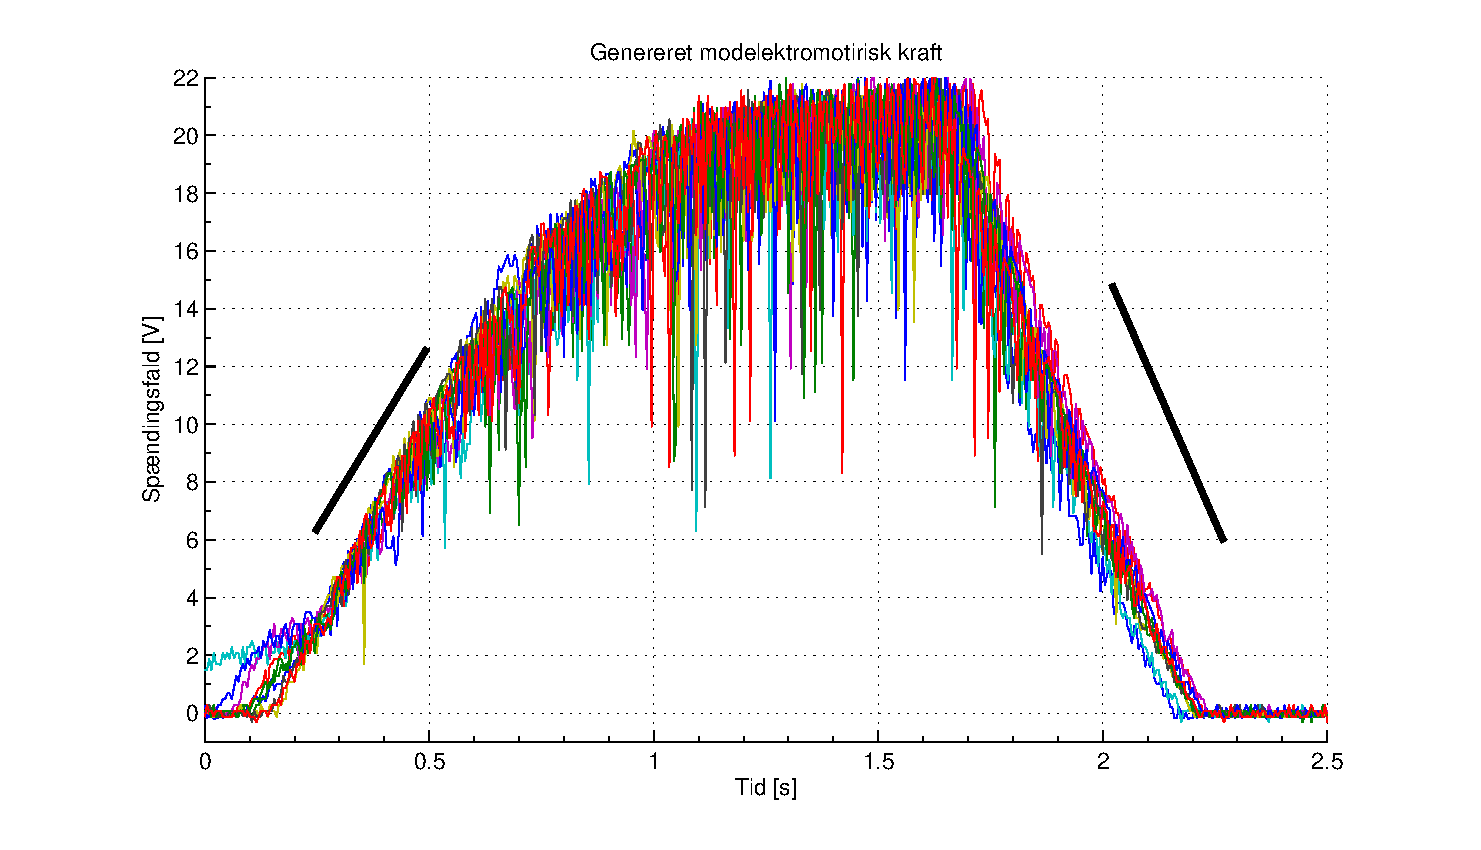
\includegraphics[width=1\textwidth]{./graphics/vemf0.eps}
	\caption[Målt modelektromotorisk kraft ved acceleration af motor]
		{Målt modelektromotorisk kraft ved acceleration af motor.
		De indtegnede sorte streger viser hældningerne før og efter loddet ramte jorden.
		På grafen vises målingerne fra flere forsøg sammen.}
	\label{fig:vemf0}
\end{figure}
\subsubsection{Databehandling}
Da målingerne er meget støjfyldte, valgtes det at lavpasfiltrere dem, så hældningsbestemmelsen
ikke bliver påvirket af den højfrekvente støj.
De lavpasfiltrerede data kan ses på figur \ref{fig:vemf1}.
\begin{figure}[th!]
	\centering
	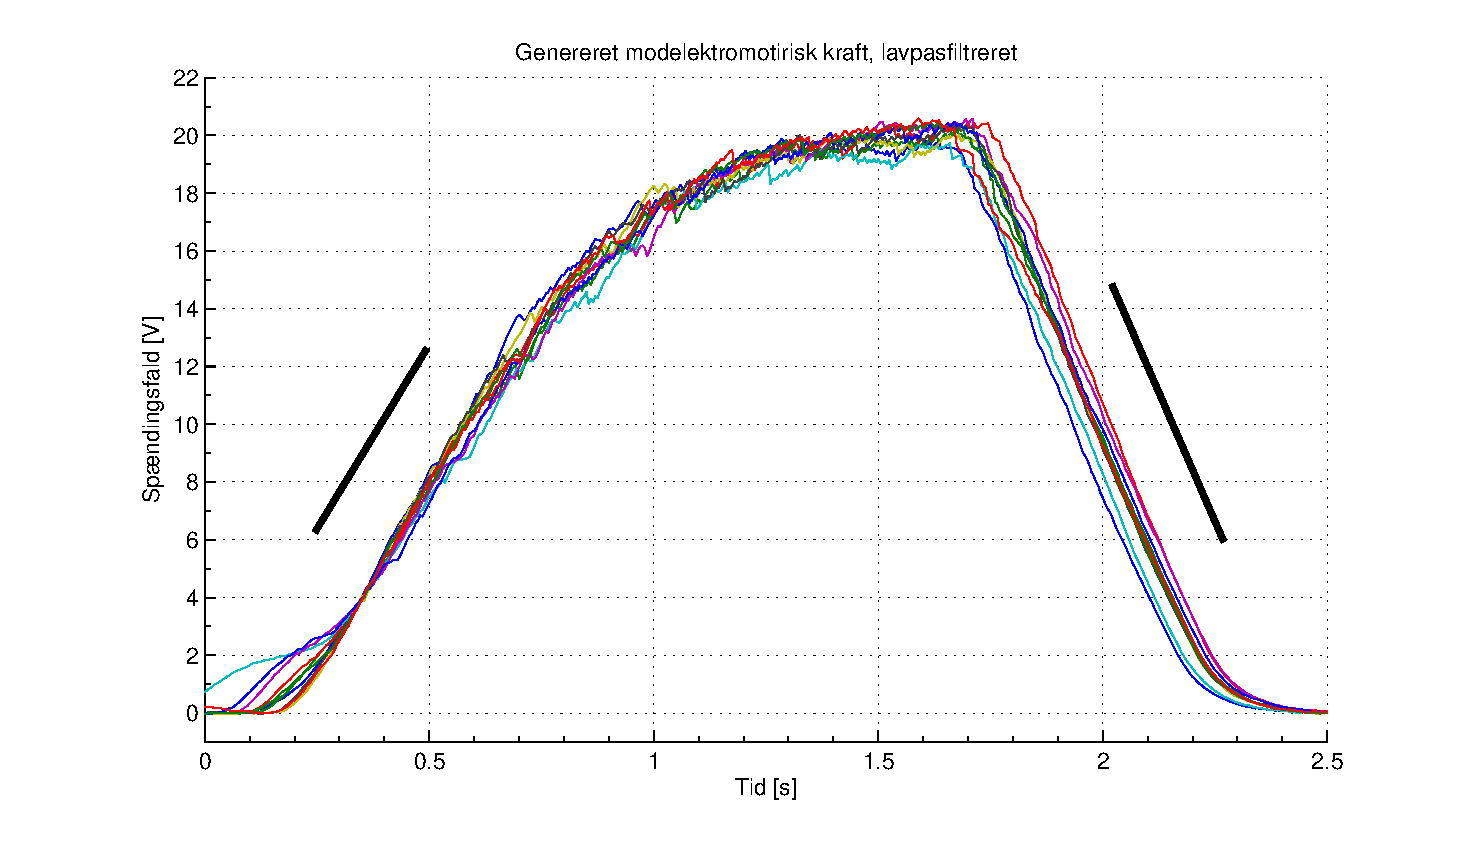
\includegraphics[width=1\textwidth]{./graphics/vemf1.eps}
	\caption[Målt modelektromotorisk kraft ved acceleration af motor, lavpasfiltreret]
		{Målt modelektromotorisk kraft ved acceleration af motor, lavpasfiltreret.
		De indtegnede sorte streger viser hældningerne før og efter loddet ramte jorden.
		På grafen vises målingerne fra flere forsøg sammen.}
	\label{fig:vemf1}
\end{figure}
Jf. ligning \ref{eq:Vm_nocurrent} er det målte spændingsfald proportionalt med
vinkelhastigheden, og hældningen af grafen vil således skulle divideres med \(K_b\),
før den repræsenterede vinkelaccelerationen. \(K_b\) blev bestemt i afsnit \ref{ss:eksperiment3}.
For hver måling bestemtes hældningerne \(\alpha_{op}\) og \(\alpha_{ned}\) vha. lineær regression på de lineære stykker,
og ud fra dette er gennemsnitsaccelerationerne blevet fundet til
\(\alpha_{op}=49,3\) \([\frac{\text{rad}}{\text{s}}]\) og \(\alpha_{ned}=-69,1\) \([\frac{\text{rad}}{\text{s}}]\).
Med disse værdier er inertimomentet beregnet vha. ligning \ref{eq:Jrotor}, og friktionskraftmomentet vha. ligning \ref{eq:Tf1}.
De beregnede værdier er hhv. \(J_m=8.26\cdot10^{-4}\) \([\text{kg}\cdot{\text{m}^2}]\) og \(\left| { T }_{ f } \right| =0,0571\) \( [\text{N} \cdot \text{m}]\).
\subsubsection{Diskussion}
At \(V_{EMF}\) aftager lineært fremfor eksponentielt indikerer,
at den viskøse friktion er lav i forhold til Coulomb-friktionen.
Den lineære approksimation der i fremgangsmåden benyttes er derfor anvendelig,
og giver et nøjagtigt billede af den tilstedeværende friktion samt rotorens inertimoment.
\subsubsection{Konklusion}
Rotorens inertimoment er bestemt til \(J_m=8,26\cdot10^{-4}\) \([\text{kg}\cdot{\text{m}^2}]\).
Friktionskraftmomentet er bestemt til \(\left| { T }_{ f } \right| =0,0571\) \( [\text{N} \cdot \text{m}]\).
\subsection{Opsummering af DC motorparameter}
\section{Beregning af inertimoment}
\label{sec:inertimomentberegning}
Dette appendiks beskæftiger sig med beregningen af de teoretiske inertimomenter
for pan- og tilt-rammerne. Der henvises til figur \ref{fig:inerti_PTS}, og
beregningerne tager udgangspunkt i rammernes mål:
\({L_{1}} =0,292\) [m],
\({L_{2}} =0,280\) [m], \({L_{3}}= 0,42\) [m], \({L_{4}} =0,246\) [m], \({L_{pro}}=0,04\) [m].

\begin{figure}[!th]
\centering
\begin{tikzpicture}[scale=0.7]
\include*{./graphics/inerti_PTS}
\end{tikzpicture}
\caption[Skitse af pan \& tilt-rammerne]{Skitse af pan \& tilt-rammerne.}
\label{fig:inerti_PTS}
\end{figure}

Den teoritiske beregning er foretaget ud fra følgende antagelser og simplificeringer:
\begin{itemize}
\item Aluminimumsprofilen, 40x40L, har en massefylde på \(\rho=1,5\) [kg/m], \citep[Kap. 2 s. 4]{alu_profil_desitet}.
\item Rammerne simplificeres som bestående af tynde stænger, således at hver ramme har to stænger, hvis bidrag
til inertimomentet kan beregnes som var de punktmasser forskudt i forhold til rotationsaksen \citep[s. 254, ligning 10.36]{fund_of_physics},
vha. ligning \ref{eq:punktmasse_para}.
\begin{equation}
J={ J }_{ com }+M\cdot { h }^{ 2 }
\label{eq:punktmasse_para} 
\end{equation}
hvor \({J_{com}} = 0\) og \(h\) er afstand til punktmassen (stangen) fra rotationsaksen.
Inertimomentet for de stænger, der står vinkelret på rotationsakserne, kan beregnes vha. ligning \ref{eq:stang}
\citep[s. 255, tabel 10-2e]{fund_of_physics}.
\begin{equation}
J=\frac { 1 }{ 12 } M\cdot { L }^{ 2 }
\label{eq:stang} 
\end{equation}
\end{itemize}

Med ovenstående formler er det muligt at finde pan og tilt-rammernes teoritiske inertimoment:
\begin{align}
\label{eq:inerti_tilt_pan}
\begin{split}
{ J }_{ tilt,1 } &= \left( \left( 1/12\cdot \rho \cdot { {L_{1}} }^{ 3 } \right) +\left( \rho \left( {L_{2}}-2\cdot {L_{pro}} \right) { \left( \frac { {L_{1}}-{L_{pro}}}{ 2 }  \right)  }^{ 2 } \right)  \right) \cdot 2
\\
 &= 0,0157499 \text{ [kg m$^2$]}
\\
{ J }_{ pan,1 }&=\left( 1/12\cdot \rho \cdot { { L }_{ 3 } }^{ 3 } \right) +\left( \rho \left( { L }_{ 4 }-{ L }_{ pro } \right) { \left( \frac { { L }_{ 3 }-{ L }_{ pro } }{ 2 }  \right)  }^{ 2 } \right) \cdot 2
\\
 &=0,0315708 \text{ [kg m$^2$]}
\end{split}
\end{align}

Tilt-rammens indflydelse på inertimomentet som pan-motoren skal rotere, er afhængig af tilt-rammens vinkel.
Når tilt-rammen er lodret er bidraget til pan-inertimomentet mindst, jf. ligning \ref{eq:punktmasse_para}, fordi afstanden
af to af stængerne til rotationsaksen (pan) er mindst. Ligeledes vil bidraget til pan-inertimomentet være størst når tilt-rammen er vandret.
Dette giver en kobling mellem pan og tilt, hvilket er uønsket under designet af reguleringssløjfen, som beskrevet i afsnit \ref{sec:matPTS}.
En simplificering er således at inkludere bidraget i modellen for pan som en konstant.
Man kan argumentere for, at denne konstant bør være gennemsnittet af bidragene for hele bevægelsen.
Denne ville kunne tilnærmes ud fra den ideelle responskurve for tilt-systemet, der kan beregnes ud fra den faste parabel, som gives som input.
Værdien ville således være baseret på ét specifikt parabelinput. En anden tilgang kunne være at vælge minimum-bidraget, og dermed
have en værdi der er nøjagtig for de tilt-vinkler, der er tæt på lodret, og mere og mere unøjagtig jo mere vandret tilit-vinklen er.
Sidstnævnte tilgang vælges, fordi tilt-vinklen i lerdueskydningen er tilnærmelsesvis lodret. Tilt-rammen roterer i vinkelintervallet \([4,03\degree \leq \phi \leq 12,3\degree]\) jf. lerduens toppunktstid samt nedslagstid på hhv. 0,557 [s] og 1,18 [s], indsat i ligning \ref{eq:sv_koordi}. Antagelsen om konstant bidrag til inertimoment er derfor nøjagtig.

Tilt-rammens bidrag til inertimomentet for pan bestemmes derfor ud fra, at to af tilt-rammens "stænger" er parallele med
rotationsaksen, og at de to stænger med længden \({L_{2}}\) er vinkelret på den, samt at de roterer om den.
Med ligningerne \ref{eq:punktmasse_para} og \ref{eq:stang}
kan tilt-rammens bidrag til pan-inertimomentet altså beregnes vha ligning \ref{eq:tiltOnPan}.
\begin{align}
\begin{split}
J_{pan,tilt_{min}}&=2\cdot{}\left(\frac{1}{12}\cdot{}\rho\cdot{}L_{2}^3
+\rho\cdot{}\left(L_1-2\cdot{}L_{pro}\right)\left(\frac{L_2-L_{pro}}{2}\right)^2\right)
\\
&=0,0146464 \text{ [kg m$^2$]}
\end{split}
\label{eq:tiltOnPan} 
\end{align}
Inertimomentet på pan-aksen er derfor givet ved summationen af pan-rammens inertimoment og tilt-rammens inertimoment,
som angivet i ligning \ref{eq:pan_inerti}.
\begin{align}
\begin{split}
{ J }_{ pan,1.1 } &= J_{ pan,1 }+J_ { pan,tilt_{ min} }
\\
&=0,0462172 \text{ [kg m$^2$]}
\end{split}
\label{eq:pan_inerti} 
\end{align}
Inertimomentet for tilt og pan er beregnet i ligning \ref{eq:inerti_tilt_pan}, mens det endelige inertimomentet for pan er beregnet i ligning \ref{eq:pan_inerti}.
Systemets gearing gør dog at inertimomenterne som motorerne belastes med, er mindre.
Gearingen i EMG30-motoren er i forholdet 30:1, mens gearingen til rammerne er i forholdet 1:3.
Ligning \ref{eq:gearing0} giver forholdet mellem det reflekterede inertimoment \(J_r\) (som motoren belastes med)
og inertimomentet \(J\) efter en gearing med forholdet \(N\) \citep{gear_inerti}.
\begin{equation}
J_r=\frac{J}{N^2}
\label{eq:gearing0}
\end{equation}
\(N\) kan altså bestemmes som multiplikationen af de to gearingsforhold, og er således lig med 10.
I ligning \ref{eq:inerti_tilt_pan_fak} er de reflekterede inertimomenter beregnet.
\begin{align}
\label{eq:inerti_tilt_pan_fak}
\begin{split}
{J_{tilt}}&=1,57499\cdot{10}^{-4} \text{ [kg m$^2$]}
\\
{J_{pan}}&=4,62172\cdot{10}^{-4} \text{ [kg m$^2$]}
\end{split}
\end{align}

\section{FPGA'ens komponenter}
\label{sec:fpgaappendix}
Dette appendix forklarer alle komponenter på FPGA'en.
Et forsimlet diagram over komponenterne på FPGA'en ses på figur \ref{fig:FPGA_blok}.


\textbf{Tic counter}\\
\textbf{Input:}
Signaler fra encoder på PTS. Reset signal fra tic reset.

\textbf{Output:} Positionen på hver af motorerne angivet i antal tics mellem 0 
og 1079. Retningen, som motorerne roterer i. 

Da encoderne på PTS er quadrature encodere er det muligt at bestemme både retning og 
tælle rotationer på motoren.
Tæller positionen op eller ned afhængigt af inputtet fra encoderne. 
Tæller ned fra 0 til 1079.
For at kalibrere positionen er det nødvendigt for tic counter komponenten at få 
et reset signal fra tic reset komponenten. 
Når dette reset signal modtages nulstilles positionen og er herved kalibreret.

\textbf{Tic reset}\\
\textbf{Input:} Signaler fra Hall sensorer på PTS. Rotationsretning.\\
\textbf{Output:} Reset signal.

\begin{figure}[!th]
\centering
\include*{./graphics/hall_sensor_signal}
\caption[Signal fra Hall sensor]{Signalet fra Hall sensor, når magneten på PTS køres hen over. Ved pilene udsendes reset signalet.}
\label{fig:hall_sensor_signal}
\end{figure}

Som beskrevet tidligere er der behov for et reset signal til positionen. 
Dette skal gøres ved hjælp af Hall sensorer på PTS. 
Det viser sig dog, at Hall sensorernes output ikke kun er højt på ét encodertick. 
Derfor kan signalet fra Hall sensorerne ikke i sig selv bruges som reset signal.
PTS rotationsretningen tages derfor med i betragtning.
Hvis PTS roterer i én retning sættes reset signalet højt på opadgående 
flanke på Hall sensor outputtet, mens reset signalet sættes højt på nedadgående 
flanke i den anden retning. Reset signalet udsendes derved på samme sted, som vist på figur \ref{fig:hall_sensor_signal}.
Hermed fås det smallest mulige område, hvor reset signalet er højt.
Præcisionen på denne kalibrering er \(\pm1\) tick.

\textbf{Display}\\
\textbf{Input:} Motorposition fra tic counter. Skaleret clock signal fra clock 
scaler.

\textbf{Output:} Signal der styrer displayet.

Modtager motorpositionen fra tic counter komponenten og viser det på de fire 8-digit-displays 
på BASYS boardet. Bruger det skalerede clock signal til at multiplexe mellem de 
fire displays.

\textbf{Clock scaler}\\
\textbf{Input:} BASYS boardets interne clock.\\
\textbf{Output:} Skaleret clock signal

Skalerer clock signalet.

\textbf{Input decoder}\\
\textbf{Input:} 16 bit data fra SPI.\\
\textbf{Output:} PWM-kanal og tilhørende PWM-duty cycle (11 bit).

Hvis setPWM bit er højt skal PWM-kanal og tilhørende PWM-duty cycle opdateres.
Opdateringen sker ved at tage 2 MSB og lave dem til et PWM-kanal output. De 11 
LSB sendes som PWM-duty cycle output.

\textbf{PWM}\\
\textbf{Input:} PWM-kanal og tilhørende PWM-duty cycle (11 bit).\\
\textbf{Output:} PWM til PTS.

Sørger for at generere PWM til PTS ud fra PWM-kanal og PWM-duty cycle.

%\subsection*{Output decoder}
\textbf{Output decoder}\\
\textbf{Input:} Motorposition fra tic counter.\\
\textbf{Output:} 16 bit data.

Sørger for skiftevis at sætte motorposition for de to motorer som LSB.
MSB bruges til at angive, hvilken motor positionen er til.

\textbf{SPI}\\
\textbf{Input:} 16 bit data fra output decoder. 16 bit data udefra.\\
\textbf{Output:} 16 bit SPI data ud.

Agerer som SPI slave i kommunikation med mikrocontrolleren.
Modtager SPI data udefra. Sørger samtidigt for at sende de 16 bit data fra output decoder.



\section{Serial Peripheral Interface}
\label{app:spi}
Kommunikationen mellem mikrocontolleren og FPGA’en foregår med Serial Peripheral Interface (SPI). 
SPI understøtter full-duplex kommunikation mellem en master og en eller flere slaver.

Der er fire kanaler mellem masteren og slaven: Slave Select (SS), Serial Clock (SCLK), Master Output Slave Input (MOSI) og Master Input Slave Output (MISO). SS bruges til at vælge hvilken slave der skal overføres data til/fra. Den kan også sammenlignes med en chip select. SCLK generes af masteren; SS, MOSI og MISO kører synkront med dette signal.

Opstillingen med en master og en slave kan ses på figur \ref{fig:SPImasterslave}. 
Her kan SS være overflødig, da der kun er en slave at vælge. Til gengæld kan SS bruges til at initialisere overførelsen. 
Når SS er sat højt, begynder overførslen mellem master og slave. Da overførslen er full-duplex sender begge til hinanden samtidig. 
\begin{figure}[!th]
\centering
\begin{tikzpicture}[scale=0.8]
\include*{./graphics/MISOMOSI}
\end{tikzpicture}
\caption[SPI protokol]{Skitse af SPI-kommunikation mellem mikrocontroller og FPGA.}
\label{fig:SPImasterslave}
\end{figure}

Når der er flere slaver, bestemmer SS hvilken slave der overføres til.
Alle slave har deres egen SS, men de deler alle MISO og MOSI. 
Før overførslen begynder sætter masteren SS høj til den ønskede slave,
derefter overføres dataene til slaven.
Mens overførslen finder sted ignorerer de ikke-valgte slaver dataene på MOSI.  
%Det er en standard hvor der bliver overført data mellem en master og en eller flere slaver. 
%Overførelsen sker med full duplex, så der bliver sendt data både fra masteren og slaven på samme tid. 

\begin{figure}[!th]
\centering
\begin{tikzpicture}[scale=0.8]
\include*{./graphics/SPIfigur}
\end{tikzpicture}
\caption[SPI overførelse]{Eksempel på en SPI overførelse.}
\label{fig:SPIfigur}
\end{figure}

Et eksempel på en overførsel mellem en master og en slave kan ses på figur \ref{fig:SPIfigur}. 
Eksemplet tager udgangpunkt i TI Synchronous Serial Frame Format Single Transfer \cite[s. 476]{lm3s6965} fra microcontrolleren.
I denne form er SSIClk, SSIFss, SSITx, SSIRx pins'ne. SSIClk er clock signalet, SSIFss er slave select og SSITx og SSITx er henholdsvis MOSI og MISO.
SCLK har en puls mere, end der er bit i hver data-frame. Det er fordi at SS går høj i den første puls, hvorefter dataene bliver sendt. 
Det gør at SS kan bruges som en indikater for at data vil blive overført.

\section{Test af mikrocontrollerens timing}
\label{sec:uctestappendix}
Dette appendix beskriver test af mikrocontrollerens timing. 
Først testes afviklingstiden for SPI funktionerne, dernæst for Control-task'en. 


SPI funktionens afviklingstid blev testet ved at skifte en digital pin før og efter SPI-funktion blev kaldt.
Et oscilloskop af typen \textit{Agilent DSO-X 2024A} blev brugt til målingerne. 

SPI funktionens afviklingstid blev på oscilloskopet målt til 40,54 [\micro s].
I løbet af 10 parabelbevægelser blev observeret en afvigelse på \(\pm2\) [ns], hvilket svarer til måleusikkerheden. 
Altså overholder implementeringen kravet på afvikling indenfor 83,3 [\micro s], som opstillet i ligning \ref{eq:uc:spi-krav}.

Samme fremgangsmåde blev brugt til at undersøge timingen for Control-task'en,
som indeholder reguleringssløjferne. Oscilloskopet blev indstillet til \(500.000\) [Samples/s].
Kravet til afviklingen var: Reguleringsløjferne kører med 600 [Hz], samt at task'en afvikles inden næste periode. 
Dvs. en maks afviklingstid på \(\frac{1}{600}\) [s], da kravet på 600 [Hz] ellers ikke kunne opfyldes. 
Intervallet mellem hver afvikling af task'en blev målt for 60 afviklinger,
og resultaterne er vist i tabel \ref{tb:ctrltasktimingtest}.
\begin{table}[h!]
% Prøv multicolummn
\centering
\begin{tabu}{l|[1.25pt]r|r|r|r}
 & Max  & Min & Median & Gennemsnit  \\ \tabucline[1.25pt]{-}
Målt interval & 1,672 [ms] & 1,662 [ms] & 1,667 [ms] & 1,667 [ms] \\ 
\hline 
Afvigelse & 5,33 [\micro s] & 4,66 [\micro s] & 0,66 [\micro s] & 0,13 [\micro s] \\
 & 0,41\% & 0,54\% & 0,03\%  & 0,03\% \\
\end{tabu} 
\caption[Interval mellem afvikling af Control task]{Interval mellem hver afvikling af Control-task. Måleusikkerheden er $\pm4$ [\micro s].}
\label{tb:ctrltasktimingtest}
\end{table}
%\todo[inline,author=Nikolaj, color=green]{Din afvigelse siger at du mangler et decimal...}

Afvigelserne for medianen og gennemsnittet ligger indenfor måleusikkerheden på $\pm4$  [\micro s].
For max. og min. værdierne er afvigelsen på max. 133\% af måleusikkerheden,
og det vurderes at denne kan negligeres. 

Samme datasæt blev brugt til at beregne afviklingstiden for task'en, koordinattransformationen og selve reguleringssløjfen. 
Disse data er vist i tabel \ref{tb:ctrl task runtime test}. %Bemærk usikkerheden på $4  [\micro s]$.

%500KSa/s
\begin{table}[h!]
\centering
\begin{tabu}{l|[1.25pt]r|r|r|r}
Afviklingstid [\micro s] & Max  &  Min & Median & Gennemsnit  \\ \tabucline[1.25pt]{-}
Ctrl task & 360  & 326  & 332  & 338  \\ \hline 
Koordinat transformation & 228  & 202  & 206  & 212  \\
\hline 
PID-regulering & 40  & 30  & 32  & 34 \\
\end{tabu} 
\captionsetup{width=0.8\textwidth}
\caption[Afviklingstiden for Control task]{Afviklingstiden for Control task, Koordinattransformation og PID-regulering. Måleusikkerheden er $\pm4$ [\micro s].}
\label{tb:ctrl task runtime test}
\end{table}

Dataene viser at Control task'en blev afviklet før sin deadline - med en margin på min. 1,294 [ms].
%\todo[inline,author=Nikolaj, color=green]{Skal man ikke tænke mindste målte interval - måleusikkerheden - længste afviklingstid? - Indregn worst case}
Variationen i afviklingstiden skyldes koordinattransformationen og PID-reguleringen. Den maksimale variation af afviklingstiden udgør $ \frac{360 - 326}{1667} = 2,04\% $ af periodetiden, hvilket kan tolereres. 

%%%%%%%%%%%% Bilag %%%%%%%%%%%%%%%
\part{Bilag}
%\section{Projektoplæg}

\begin{figure}[th!]
\centering
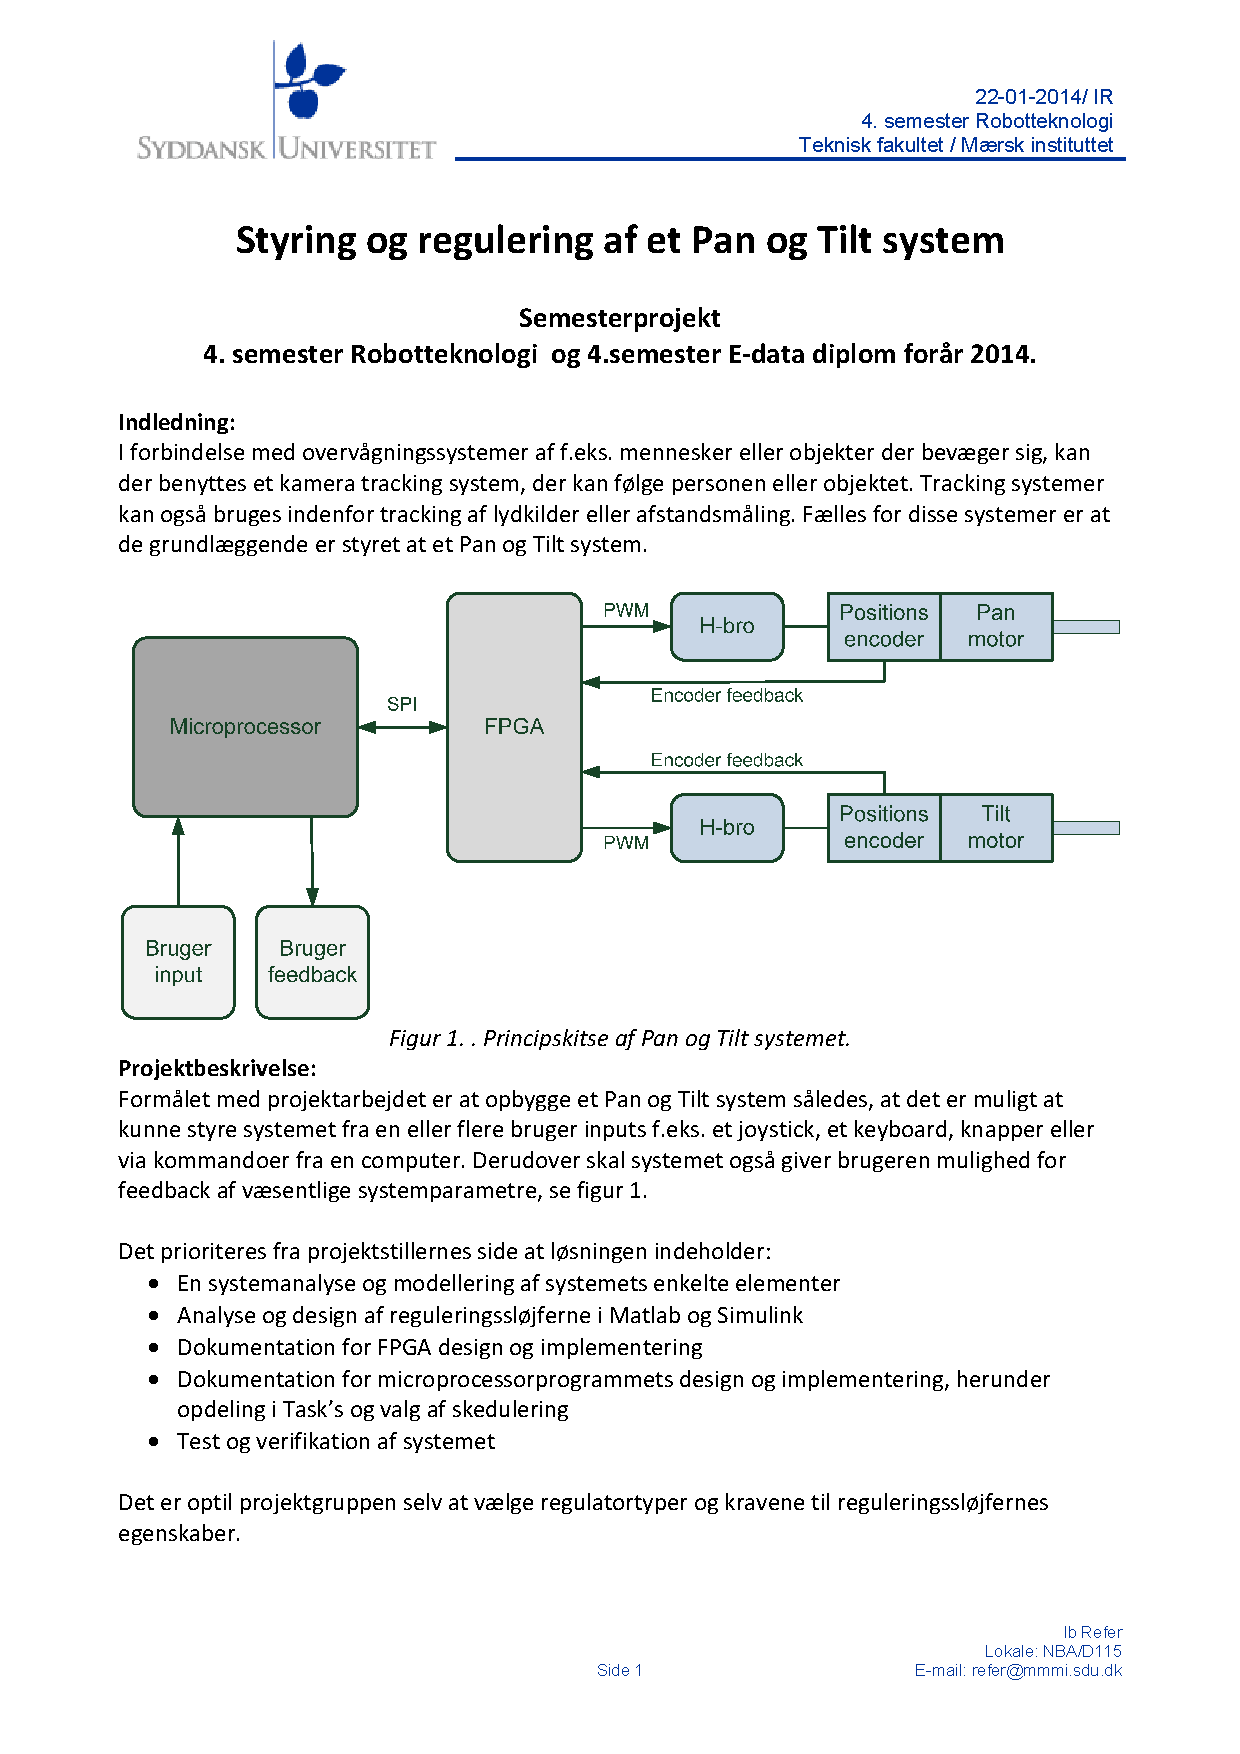
\includepdf[scale=0.82]{./content/Projekt_2014-1.pdf}
\end{figure}
\newpage
\begin{figure}[th!]
\centering
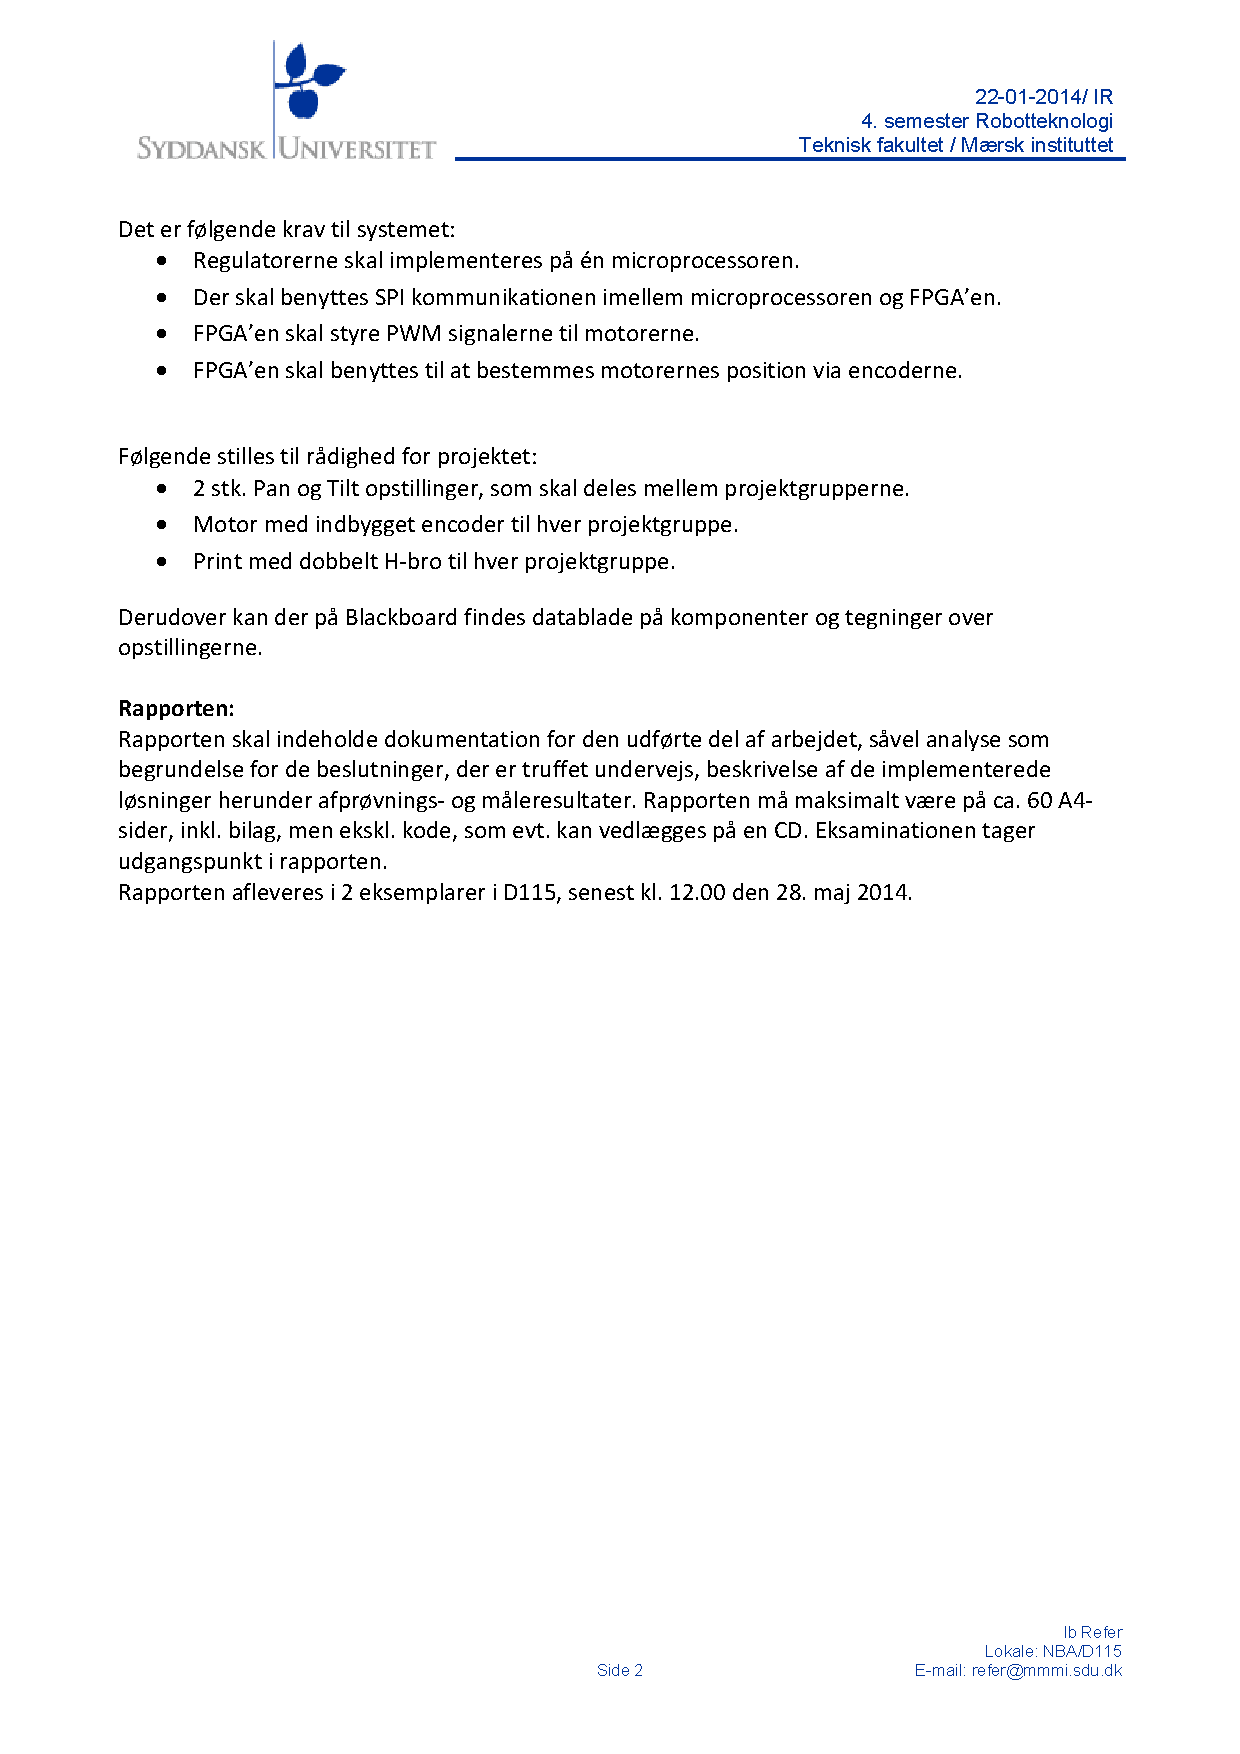
\includepdf[scale=0.82]{./content/Projekt_2014-2.pdf}
\end{figure}



\end{document} 
